% cSpell:disable

\documentclass[12pt,letterpaper]{report}

% cSpell:disable

\usepackage{style/buthesis}
\usepackage[utf8]{inputenc}

\usepackage[usenames,dvipsnames]{xcolor}
\usepackage[
	lambda,
	advantage,
	operators,
	sets,
	landau,
	probability,
	notions,
	logic,
	ff,
	mm,
	primitives,
	events,
	complexity,
	asymptotics,
	keys
]{cryptocode}
\usepackage{appendix}
\usepackage{amsmath}
\usepackage{amsfonts}
\usepackage{subcaption}
\usepackage{graphicx}
\usepackage{balance}
\usepackage{mathtools}
\usepackage{nicefrac}
\usepackage{booktabs}
\usepackage{multirow}
\usepackage{bm}
\usepackage{rotating}
\usepackage[
	colorlinks = true,
	linkcolor = Fuchsia,
	urlcolor  = JungleGreen,
	citecolor = magenta
]{hyperref}
\usepackage{cleveref} % must be loaded after hyperref

\usepackage{color}
\usepackage{amsthm}
\usepackage{caption}
\usepackage[all]{nowidow}
\usepackage{hyphenat}
\usepackage[inline]{enumitem}
\usepackage{siunitx}
\usepackage[mathscr]{eucal}

\usepackage[
	backend=biber,
	style=alphabetic,
	giveninits=true,
	sorting=ydnt,
	maxbibnames=1000,
	maxalphanames=4
]{biblatex}

\bibliography{bibfile}

\renewcommand*{\mkbibnamegiven}[1]{%
	\ifitemannotation{highlight}
	{\textbf{#1}}
	{#1}
}

\renewcommand*{\mkbibnamefamily}[1]{%
	\ifitemannotation{highlight}
	{\textbf{#1}}
	{#1}
}

\graphicspath{{./graphics/}}

\ifdefined\draft%
	% https://www.overleaf.com/learn/latex/Inserting_Images#Generating_high-res_and_low-res_images
	\usepackage{epstopdf}
	\epstopdfDeclareGraphicsRule{.pdf}{png}{.png}{convert #1 \OutputFile}
	\DeclareGraphicsExtensions{.png,.pdf}
\fi

\usepackage[
	acronym,
	nonumberlist,
	nopostdot,
	nogroupskip
]{glossaries}
\renewcommand*{\glsclearpage}{}
\renewcommand*{\acronymname}{List of Abbreviations}

\newglossarystyle{gloTable}
{%
	\renewenvironment{theglossary}%
		{
			\begin{center}
				\begin{longtable}{lll}
		}%
		{
				\end{longtable}
			\end{center}
		}%
	\renewcommand*{\glossaryheader}{
		\hspace*{2em} & \hspace*{\dimexpr\textwidth-2em-4.5in\relax} & \hspace*{4.5in} \tabularnewline%
	}%
	% no group headings:
	\renewcommand*{\glsgroupheading}[1]{}%
	% main (level 0) entries displayed in a row
	\renewcommand{\glossentry}[2]{%
		\glsentryitem{##1}\glstarget{##1}{\textbf{\glossentryname{##1}}} & \dotfill & \glossentrydesc{##1} \tabularnewline%
	}%
	% sub-entries (same as main)
	\renewcommand{\subglossentry}[3]{\glossentry{##2}{##3}}%
	% blank row between groups if nogroupskip=false
	\ifglsnogroupskip%
		\renewcommand*{\glsgroupskip}{}%
	\else
		\renewcommand*{\glsgroupskip}{ & & \tabularnewline}%
	\fi
}
\setglossarystyle{gloTable}

\renewcommand*{\glsclearpage}{}
\makeglossaries%
\glsaddall%

\newcommand{\crypte}{Crypt$\epsilon$}
\newcommand{\epsolute}{\ensuremath{\mathcal{E}}psolute}

\newcommand{\record}{\ensuremath{r}}
\newcommand{\recordID}{\ensuremath{\record^\mathsf{ID}}}
\newcommand{\recordIDPrime}{\ensuremath{{}^\mathsf{ID}\record^\prime}}
\newcommand{\querySet}{\ensuremath{\mathcal{Q}}}
\newcommand{\queryKey}{\ensuremath{K}}

\newcommand{\domainSize}{\ensuremath{N}}
\newcommand{\dataSize}{\ensuremath{n}}
\newcommand{\oramsNumber}{\ensuremath{m}}

\newcommand{\user}{\ensuremath{\mathscr{U}}}
\newcommand{\client}{\ensuremath{\mathscr{C}}}
\newcommand{\server}{\ensuremath{\mathscr{S}}}

\newcommand{\protocol}{\ensuremath{\Pi}}
\newcommand{\protocolSetup}{\ensuremath{\protocol_{\mathsf{setup}}}}
\newcommand{\protocolQuery}{\ensuremath{\protocol_{\mathsf{query}}}}
\newcommand{\protocolNoGamma}{\ensuremath{\protocol_{\mathsf{no-}\gamma}}}
\newcommand{\protocolGamma}{\ensuremath{\protocol_\gamma}}

\newcommand{\searchKey}{\textsf{SK}}
\newcommand{\searchKeyDomain}{\ensuremath{\mathcal{X}}}

\newcommand{\serverDS}{\ensuremath{\mathcal{DS}}}
\newcommand{\indexI}{\ensuremath{\mathcal{I}}}
\newcommand{\database}{\ensuremath{\mathcal{D}}}
\newcommand{\databaseDef}{\ensuremath{\database = \allowbreak \{(\record_1, \allowbreak \recordID_1, \allowbreak \searchKey_1), \allowbreak \ldots, \allowbreak (\record_\dataSize, \allowbreak \recordID_\dataSize, \allowbreak \searchKey_\dataSize)\}}}
\newcommand{\fanout}{\ensuremath{k}}

\newcommand{\oram}{\ensuremath{\textsc{ORAM}}}
\newcommand{\oramProgram}{\ensuremath{\mathbf{y}}}
\newcommand{\oramRead}{\ensuremath{\mathbf{r}}}
\newcommand{\oramWrite}{\ensuremath{\mathbf{w}}}

\newcommand{\efficiencyCoefficient}{\ensuremath{a_1}}
\newcommand{\efficiencyOffset}{\ensuremath{a_2}}

\DeclareDocumentCommand{\algo}{ m g }{%
	{%
		\textsc{#1}%
		\IfNoValueF{#2}{\ensuremath{\left( #2 \right)}}%
	}%
}

\DeclareDocumentCommand{\query}{ g g }{%
	{%
		\IfValueTF{#2}%
			{\ensuremath{q_{\interval{#1}{#2}}}}%
			{
				\IfValueTF{#1}%
					{\ensuremath{q_{#1}}}%
					{\ensuremath{q}}
			}%
	}%
}

\newcommand{\adversary}{\ensuremath{\mathcal{A}}}
\newcommand{\leakage}[1]{\ensuremath{\mathcal{L}_{\textsf{#1}}}}
\renewcommand{\simulator}{\textsc{Sim}}
\DeclareDocumentCommand{\view}{ g g }{%
	{%
		\IfValueTF{#2}%
			{\ensuremath{\algo{View}_{#1} \left( #2 \right)}}%
			{
				\IfValueTF{#1}%
					{\ensuremath{\algo{View}_{#1}}}%
					{\ensuremath{\algo{View}}}
			}%
	}%
}

\providecommand{\bigTheta}[1]{\ensuremath{\Theta \left( #1 \right)}}

\newcommand{\fromNtoM}[3]{\ensuremath{#1_#2, \ldots, #1_#3}}
\newcommand{\probability}[1]{\ensuremath{\textnormal{Pr}\left[ #1 \right]}} % chktex 35

\newcommand{\efficiency}[2]{\ensuremath{\left( \bigO{ #1 }, \ifthenelse{\equal{#2}{0}}{#2}{\bigO{ #2 }} \right)}}

\newcommand{\semitransp}[2][35]{\color{fg!#1}#2}

\newcommand{\BPlus}{B\raisebox{.35\height}{\scalebox{.8}{+}}}
\newcommand{\IO}{I/O}
\newcommand{\knn}{\ensuremath{k}NN}


\glssetwidest{NEUROD    } % widest name

\newacronym%
	{aws}
	{AWS}
	{Amazon Web Services}

\newacronym%
	{gcp}
	{GCP}
	{Google Cloud Platform}

\newacronym%
	{vm}
	{VM}
	{Virtual Machine}



\begin{document}

	% cSpell:ignore pdftitle pdfsubject pdfkeywords pdfcreator pdfproducer dvips Epsolute

\title{Secure and Efficient Query Processing in Outsourced Databases}
\author{Dmytro Bogatov}

\degree=2

\prevdegrees{
	B.S., Worcester Polytechinc Institute, 2017 \\
	M.S., Boston University, 2019
}

\department{Graduate School of Arts and Sciences}

\defenseyear{2022}
\degreeyear{2022}

\reader{First}{George Kollios, Ph.D.}{Professor of Computer Science}{{\Fontskrivan\slshape\setul{0.1ex}{}\ul{~~Approved~~}}} % chktex 6
\reader{Second}{Leonid Reyzin, Ph.D.}{Professor of Computer Science}{{\calligra\setul{0.1ex}{}\ul{~~Approved~~}}}
\reader{Third}{Manos Athanassoulis, Ph.D.}{Assistant Professor of Computer Science}{{\cursive\setul{0.1ex}{}\ul{~~Approved~~}}}
\reader{Fourth}{Adam O'Neil, Ph.D.}{Assistant Professor of Computer Science, UMass Amherst}{{\wedn\setul{0.1ex}{}\ul{~~Approved~~}}}

\numadvisors=1
\majorprof{George Kollios, Ph.D.}{Professor of Computer Science}

% TODO conditionally uncomment for print
% \buecethesistitleboxpage

\hypersetup{
	pdfauthor   = {Dmytro Bogatov <dmytro@bu.edu>},
	pdftitle    = {Secure and Efficient Query Processing in Outsourced Databases},
	pdfsubject  = {Doctoral Dissertation},
	pdfkeywords = {OPE, ORE, Range Query Protocols, Epsolute, kNN},
	pdfcreator  = {LaTeX with hyperref package},
	pdfproducer = {dvips + ps2pdf}
}


	\ifthenelse{1=1}{
		\maketitle
	}{
		Not particularly proud, but it seems necessary.
		I use pandoc to convert Tex to text and then run some plain text analysis.
		For some reason pandoc fails for the \\maketitle statement.
		However, it is not smart enough to deduce that this condition is always true, while Tex is.
	}
	\cleardoublepage%

	\copyrightpage%
	\cleardoublepage%

	\approvalpage%

	\cleardoublepage%

	\IfFileExists%
		{frontmatter/quote.tex}
		{
			\ifx\noAcks\undefined%
				\newpage
				{
	\null\vfill

	\newlength\longest%
	\settowidth\longest{\LARGE\itshape{} Ask not what your country can do for you ---}
	\centering
	\parbox{\longest}{%
		\raggedright{\LARGE\itshape%
			Ask not what your country can do for you --- \\
			ask what you can do for your country.\/\par\bigskip
		}
		\raggedleft\Large\MakeUppercase{John Fitzgerald Kennedy}\par%
	}

	\vfill\vfill
}

				\cleardoublepage%
			\fi
		}
		{}

	\IfFileExists%
		{frontmatter/dedication.tex}
		{
			\ifx\noAcks\undefined%
				\newpage
				\section*{\centerline{Dedication}}

	I dedicate my dissertation work to my wife, my parents and the brave defenders of Ukraine.
	Dasha, love of my life, thank you for supporting me since the very first day of the program, through the long distance, once-in-a-century world-wide health crisis and the war.
	It was with your help that I was able to come so far.
	A special feeling of gratitude to my loving parents, Kostiantyn and Nataliia, whose help early in my academic career was critical and enabled my doctorate program in the first place, and whose support never waned to this day.
	Lastly, my heart and my thoughts go to the brave people of Ukraine, who are heroically defending the motherland from Russian invasion with their lives.
	We are with you, physically and virtually, in Lviv and Mariupol, in Kharkiv and in Kyiv.
	My sincere hope, my wish, is that this work will contribute, however little, to the cause of my beloved nation.
	Слава Україні!

				\cleardoublepage%
			\fi
		}
		{}

	\IfFileExists%
		{frontmatter/acknowledgments.tex}
		{
			\ifx\noAcks\undefined%
				\newpage
				\section*{\centerline{Acknowledgments}}

	First and foremost, I want to thank my advisor, George Kollios, for his guidance and continued support throughout my doctorate journey, from the day he accepted me to his lab to this day.
	I am honored to call him and his family my friends.
	I also thank Leo Reyzin for the time and effort he spent helping me with my work, and for the many cups of coffee and long life talks we have had over these years.
	I want to especially note the many hours-long philosophical discussions with Manos Athanassoulis --- the discussions I truly enjoyed.
	In the heat of the our debates we have lived up to the Ph.\ part of our degrees.
	My special thanks go to Adam O'Neil for his countless contributions to my works.
	He has been an invaluable co-author, contributor, reviewer and friend.

	I would like to express my gratitude to my closest ally in this life, my beloved wife, Daria Bogatova.
	There is not a single piece fo writing I did without your review, not a single figure I crafted without your keen eye refining the tiniest details, from fonts to colors.
	Even the source code of this very thesis has been branched off of your work Bachelor work \cite{dasha-thesis}.
	You are the first to listen to my ideas, and the first to support them unconditionally.

	% - George
	% - Leo
	% - Manos
	% - Adam
	% - Dasha + citation
	% - Sasha
	% - Kellaris
	% - Bjorn and IBMers
	% - Kobbi, Hamed
	% - Kiran, Sriram, Naresh
	% - Family
	% - Larger family
	% - Cat

				\cleardoublepage%
			\fi
		}
		{}

	\begin{abstractpage}
		As organizations struggle with processing vast amounts of information, outsourcing sensitive data to third parties becomes a necessity.
To protect the data, various cryptographic techniques are used in outsourced database systems to ensure data privacy while allowing efficient querying.

In this prospectus, I propose a definition and components of a new secure and efficient outsourced database system, which answers various types of queries, with different privacy guarantees in different security models.
I start with my survey work on five order-preserving and order-revealing encryption schemes that can be used directly in many database indices, like the B+ tree, and five range query protocols with various trade-offs in terms of security and efficiency.
This work systematizes the state-of-the-art range query solutions in a snapshot adversary setting and offers some non-obvious observations regarding the efficiency of the constructions.
I then follow with a recently published work, \epsolute{}, an efficient range query engine in a persistent adversary model.
In this work, we achieve security in a setting with a much stronger adversary where she can continuously observe everything on the server, and leaking even the result size can enable a reconstruction attack.
We propose a definition, construction, analysis and experimental evaluation of a system that provably hides both access pattern and communication volume, while remaining efficient.
Finally, I describe an ongoing work on secure \acrlong{knn} queries, in which the security is achieved similarly to \acrshort{ope}/\acrshort{ore} solutions --- encrypting the input with an approximate \acrlong{dcpe} scheme, so that the inputs are perturbed, but the query algorithm still produces accurate results.

	\end{abstractpage}
	\cleardoublepage%

	\setcounter{tocdepth}{4}
	\phantomsection%
	\addcontentsline{toc}{chapter}{Contents}
	\tableofcontents
	\cleardoublepage%

	\newpage
	\listofalgorithms%
	\addcontentsline{toc}{chapter}{\listalgorithmname}
	\cleardoublepage%

	\newpage
	\listoftables
	\addcontentsline{toc}{chapter}{\listtablename}
	\cleardoublepage%

	\newpage
	\listoffigures
	\addcontentsline{toc}{chapter}{\listfigurename}
	% \cleardoublepage%

	\addtocontents{toc}{\protect\contentsline{chapter}{\protect{}List of Acronyms}{xx}{link}}
	\printglossaries%
	\cleardoublepage%

	\newpage
	\endofprelim%
	\cleardoublepage%

	\chapter{Introduction}\label{section:introduction}

\thispagestyle{myheadings}

	\section{A few remarks before you start}\label{section:introduction:history}

		Intro goes here  \Gls{ad}.
		And one reference~\cite{practical-ore}.

		\begin{figure}[hb]
	\centering
	
\includegraphics[width=0.33\textwidth]{goethe}
	\caption[Short caption]{
		Long caption.
		Multiline.
	}\label{figure:goethe}
\end{figure}


		Reference to \cref{figure:goethe}.

		And one \href{https://dbogatov.org}{link}.

	\cleardoublepage%
	\chapter{Background}\label{section:background}
\thispagestyle{myheadings}

	In this section, I will go over the building blocks required to construct the outsourced database systems and their components that I will discuss in the next chapters.
	These prerequisites include the symmetric encryption, \acrshortpl{oram} and PathORAM \cite{path-oram} in particular, \acrlong{dp} and \acrshort{dp} sanitizers, and finally, \acrlongpl{tee}.
	\emph{Some of the following sections were paraphrased or taken verbatim from my published work \cite{ore-benchmark-17,epsolute}.}

	\section{Symmetric encryption}\label{section:background:encryption}

		Symmetric encryption scheme is a tuple of algorithms $\algo{E} = \{ \algo{KeyGen}, \algo{Enc}, \algo{Dec} \}$ with the following properties.
		$\algo{E.KeyGen} \left( \secparam \right) \to \key$ is a \emph{randomized} algorithm that on a security parameter $\secparam$ returns a key that will be used for both encryption and decryption.
		$\algo{E.Enc} \left( m \right) \to c$ is a \emph{randomized} algorithm that on a plaintext message $m \in \bin^*$ produces its ciphertext $c \in \bin^*$.
		$\algo{E.Dec} \left( c \right) \to m$ is a \emph{deterministic} algorithm that on a ciphertext $c \in \bin^*$ produces its original plaintext message $m \in \bin^*$.

		\subsection{Security}

			The security of the symmetric encryption is typically defined as the indistinguishability under a certain attack.
			The definition is structured around the game between the challenger and the adversary \adversary{}.
			The challenger fixes one of the two ``worlds'', left or right, and the adversary wins the game if she can reliably tell which world it was.

			A weaker security definition, \acrfull{ind-cpa}, intuitively, requires that the ciphertext leaks nothing about the plaintext.
			To formalize the requirement, the adversary can give the challenger a set of plaintext pairs to encrypt, and the challenger responds with a set of ciphertexts where the left or the right part was encrypted.
			The adversary can then use any (polynomial) algorithm over the ciphertexts and make a guess of whether the left or the right part was encrypted.
			The claim is, if there is anything that the ciphertext leaks about the plaintext, there exists an adversary who will win.
			The security claim is therefore contrapositive --- the scheme is \acrshort{ind-cpa} secure iff there is no such adversary that wins the game.
			The \acrshort{ind-cpa} definition can be upgraded to allow the adversary to choose the plaintexts adaptively (\acrshort{cpa}2), or require the ciphertext be indistinguishable from a random bit-string (\acrshort{cpa}\$).

			\acrshort{ind-cpa} security is not by itslef sufficient since it does not account for the decryption part of the scheme.
			There are known attacks that decrypt the plaintext (i.e., defeat the encryption) if the adversary can trigger the decryption and observe the process or the result (see padding attack \cite{padding-attack} and \acrshort{xml} encryption attack \cite{xml-break-encryption}).

			The stronger definition, \acrfull{ind-cca}, captures the decryption component.
			It extends the \acrshort{ind-cpa} game in that the adversary can now request the challenger to decrypt \emph{any} ciphertext of her choice \emph{except} the ones that the chalenger himself encypted for the adversary.
			The adversary still outputs a guess of the two worlds and wins if reliably guesses correctly.
			Note that in this game if the decryption can fail for any reason, or even if \adversary{} can observe any difference in execution for different inputs, the scheme is insecure.
			Therefore, \acrshort{ind-cca} immediately rules out the aformentioned attacks \cite{padding-attack,xml-break-encryption}.
			Similarly to \acrshort{ind-cpa}, \acrshort{ind-cca} also has the adaptive and indistinguishable\hyp{}from\hyp{}pseudorandom variants \acrshort{cca}2 and \acrshort{cca}\$.

		\subsection{Components}

			Note that for the practical purposes I define the encryption algorithm as randomized --- producing different ciphertext for the same plaintext on every invocation.
			While this is how the symmetric encryption scheme is used in applications, formally, producing the deterministic ciphertext and randomizing it are different operations.

			Internally, the encryption scheme typically consists of a keyed \acrfull{prp} (also known as a \emph{block cipher}), a \acrfull{prg} that is used to generate a (pseudo)random \acrfull{iv} and a block cipher \emph{mode of operation}.\footnote{% chktex 36
				Here I describe the \emph{block ciphers} family of symmetric encryption algorithms.
				Streaming ciphers are not used in this thesis.
			}
			First, the input $m \in \bin^*$ is split into blocks (depending on the underlying block cipher, for example, 128 bits) and the last block is padded if necessary.
			Second, the pseudorandom \acrlong{iv} of size of the block is generated with a \acrshort{prg}.
			Intuitively, this is the part that contributes the  ``randomness'' to the process.\footnote{
				There are some modes of operation that do not require the \acrlong{iv}, such as \acrfull{ecb} mode, but these are insecure.
			}
			Finally, the \acrshort{iv} is prepended to the plaintext blocks and the algorithm applies the permutation to one block at a time with the input masked according to the mode of operation.
			The resulting object is a ciphertext that is one block longer than a plaintext due to \acrshort{iv}.
			In practical systems, the ciphertext is then broken up into components, like the ciphertext material itself, the \acrshort{iv}, the version of the key, etc.
			Also note that the encryption scheme key has a maximum number of times it can be used for encryption (its \emph{operational lifetime}).

			\acrfull{aes} \cite{aes-nist} is a \acrshort{nist}-standardized block cipher, which, along with the standardized mode of operation \cite{nist-modes} and \acrshort{prg} \cite{nist-prg} used to generate the \acrshort{iv}, forms the symmetric encryption system.

	\section{\texorpdfstring{\acrlong{oram}}{Oblivious Random Access Machine}}\label{section:background:oram}

		Informally, \acrfull{oram} is a mechanism that lets the users hide their access pattern to remote storage.
		An adversarial server can monitor the actual accessed locations, but she cannot tell a read from a write, the content of the block or even whether the same logical location is being referenced.
		The notion was first defined by \textcite{oram-theory} and \textcite{oram-original}.

		More formally, a $(\eta_1, \eta_2)$-\acrshort{oram} protocol is a two-party protocol between a client \client{} and a server \server{} who stores a memory array.
		In each round, the client \client{} has input $(o, a, d)$, where $o$ is an access type (\oramRead{} or \oramWrite{}), $a$ is a memory address and $d$ is a new data value, or $\bot$ for read operation.
		The input of \server{} is the current array.
		Via the protocol, the server updates the memory or returns to \user{} the data stored at the requested memory location, respectively.
		We speak of a sequence of such operations as a program \oramProgram{} being \emph{executed under the \acrshort{oram}}.

		An \acrshort{oram} protocol must satisfy correctness and security.
		Correctness requires that \client{} obtains the correct output of the computation except with at most probability $\eta_1$.
		For security, we require that for every client \client{} there exists a simulator $\simulator_\oram$ which provides a simulation of the server's view in the above experiment given only the number of operations.
		That is, the output distribution of $\simulator_\oram (c)$ is indistinguishable from $\algo{View}_\server$ with probability at most $\eta_2$ after $c$ protocol rounds.
		Note that the \acrshort{oram} protocols typically differ in the way the storage is organized and manipulated, but are similar in that the records or blocks are symmetrically encrypted (see \cref{section:background:encryption}).

		\acrshort{oram} protocols are generally stateful, after each execution the client and server states are updated.
		\emph{For brevity, throughout the thesis I will assume the \acrshort{oram} state updates are implicit, including the encryption key generated and maintained by the client.}

		Some existing efficient \acrshort{oram} protocols are Square Root \acrshort{oram} \cite{oram-theory}, Hierarchical \acrshort{oram} \cite{oram-original}, Binary-Tree \acrshort{oram} \cite{binary-tree-oram}, Interleave Buffer Shuffle Square Root \acrshort{oram} \cite{shortest-path-oram}, TP-ORAM \cite{tp-oram}, PathORAM \cite{path-oram} and TaORAM \cite{taostore}.
		For detailed descriptions of each protocol, I recommend the work of \textcite{oram-survey-feifei}.
		The latter three \acrshortpl{oram} achieve the lowest communication and storage overheads, $\bigO{\log \dataSize}$ and \bigO{\dataSize}, respectively.

		\subsection{PathORAM}

			PathORAM \cite{path-oram} is one of the most commonly used \acrshort{oram} protocols due to its efficiency and simplicity.
			In this section I briefly describe this construction as it is used as an \acrshort{oram} instantiation in the rest of the thesis.

			In the PathORAM, both the client \client{} and the server \server{} are stateful.
			The server stores the encrypted records (blocks) grouped in buckets, and the buckets form a binary tree.
			The client's storage, although asymptotically linear in the data size, is relatively small in practice.
			The client stores the \emph{position map} that maps the record ID to a leaf in the server tree storage and a small amount of stash, which can store some plaintext blocks on the client side.

			The main invariant of the protocol is that at all times the ciphertext of the record $a$ is stored somewhere on the \emph{path} from the root to the leaf that is mapped to $a$, or in the stash (hence the name of the construction).

			The \acrshort{oram} is initialized with a binary tree of buckets with all buckets containing valid encryptions of dummy records.
			The position map is sampled at random (filled with permuted distinct numbers).

			Main routine of the \acrshort{oram} is an access sub-protocol, which is similar for read \oramRead{} and write \oramWrite{} type of access (remember, \acrshort{oram} hides the type of access from the curious server).
			In PathORAM, the access $(o, a, d)$ consists of four steps.
			First, remap the current leaf $x$ for $a$ to a new random leaf $x^\prime$.
			Second, read the entire path to leaf $x$ (all buckets from root to leaf) into the client stash.
			Third, the client updates the block value to $d$ if the access is a write \oramWrite{}.
			Finally, write back the path to leaf $x$ filling the buckets with all blocks from stash in a way that maintains the invariant.

			The newly updated block $a$ with the new value $d$ may be included in the new path, or it may stay in the stash.
			It is important that the stash size be provably bounded.
			\cite[Theorem 1]{path-oram} does exactly that --- at least for the bucket size of 5, the probability of stash overflow and its size are related as in \cref{equation:path-oram-stash}.
			\begin{equation}\label{equation:path-oram-stash}
				\probability{ \mathsf{stash\ size} > x } \leq 14 \cdot (0.6002) ^ x
			\end{equation}
			If the probability of a protocol failure is thought of as the adversary's advantage (the probability to break the security), then the stash size equivalent to 128-bit security is about 100 blocks for the bucket of size 5 \cite[Figure 5]{path-oram}.

	\section{\texorpdfstring{\acrlong{dp}}{Differential Privacy}}

		\acrfull{dp} is a guarantee on a mechanism that takes a dataset and returns some result.
		The guarantee states that for two neighboring databases (that differ in exactly one record), the probability that the adversary will understand by looking at the output, which of the two databases was used as an input, is bounded.
		More formally, the \acrlong{dp} is defined in \cref{definition:dp}.

		\begin{definition}[\acrlong{dp}, adapted from \cite{our-data-ourselves, differential-privacy-original}]\label{definition:dp}
			A randomized algorithm \algo{A} is $(\epsilon, \delta)$-differentially private if for all $\database_1 \sim \database_2 \in \searchKeyDomain^\dataSize$, and for all subsets $\mathcal{O}$ of the output space of \algo{A},
			\[
				\probability{ \algo{A}{ \database_1 } \in \mathcal{O} } \leq \exp(\epsilon) \cdot \probability{ \algo{A}{ \database_2 } \in \mathcal{O} } + \delta \; .
			\]
		\end{definition}

		One way to interpret this definition is the following.
		Probabilities are taken over the coins of algorithm \algo{A}, which answers a query based on a dataset.
		A natural instantiation of \algo{A} is a view of a distinguishing adversary \adversary{}, who tries to guess which of the two datasets was used.
		The expression in \cref{definition:dp} then bounds the advantage of \adversary{} with $\epsilon$ and $\delta$ parameters.
		Note that $\exp( x ) \approx 1 + x + \frac{x^2}{2!}$, and for sufficiently small $x$ the last term is negligible.
		If we put $\epsilon + 1$ in place of $\exp( \epsilon )$, it becomes clear that $\epsilon$ is the exact value by which two probabilities are allowed to differ.
		For $\epsilon = 0$, they have to be equal, for $\epsilon = 0.01$, probabilities may differ by \SI{1}{\percent}.
		Therefore, $\epsilon$ is called \emph{a privacy budget} of a \acrshort{dp} system.
		$\delta$ term is additive and therefore must be small by itself.
		This term is essentially a probability that the entire system fails.
		For example, if \algo{A} is a randomized algorithm that fails with a certain chance, this probability will be $\delta$.
		For instance, a PathORAM \cite{path-oram} algorithm can have a stash overflow with a bounded probability \cite[Theorem 1]{path-oram} and it will cause the entire algorithm to fail.
		If PathORAM is used in a \acrshort{dp} system then this probability, however small, bounded and negligible, will have to be accounted for in $\delta$.

		Note that \cref{definition:dp} describes a property of \algo{A} and not a construction method.
		To construct \algo{A}, the seminal work of \textcite{differential-privacy-original} offers an algorithm called \acrfull{lpa}.
		The idea is to tune the noise sampled from the Laplacian distribution to the \emph{sensitivity} of a query, defined as the change of output with respect to change in input.
		For example, if a change in one record of the dataset causes a change in the output value of at most one (e.g., a count query), then the sensitivity is 1.
		\cite{differential-privacy-original} proves that if one adds $\algo{Laplace}{0, \frac{\mathsf{sensitivity}}{\epsilon}}$ to the real result of a query, the resulting mechanism is $\epsilon$-\acrshort{dp}.

		\subsection{\texorpdfstring{\acrshort{dp}}{DP} sanitizers}\label{section:background:dp-sanitizers}

			While the \acrlong{lpa} is an effective and simple way of answering a single count query, we will need to answer a sequence of count queries, ideally, without imposing a bound on the length of this sequence.
			We will hence make use of \emph{sanitization} algorithms.

			\begin{definition}\label{definition:dp-danitizer}
				Let \querySet{} be a collection of queries.
				An $(\epsilon, \delta, \alpha, \beta)$-differentially private sanitizer for \querySet{} is a pair of algorithms $(\algo{A}, \algo{B})$ such that:
				\begin{itemize}
					\item $A$ is $(\epsilon, \delta)$-differentially private, and
					\item on input a dataset $\database = \fromNtoM{d}{1}{\dataSize} \in \searchKeyDomain^\dataSize$, \algo{A} outputs a data structure \serverDS{} such that with probability $1 - \beta$ for all $\query \in \querySet$, $\abs{ \algo{B}{ \serverDS, \query } - \sum_i \query(d_i) } \leq \alpha$.
				\end{itemize}
			\end{definition}

			\begin{remark}\label{remark:dp-sanitizer-guarantees}
				Given an $(\epsilon, \delta, \alpha, \beta)$-\acrshort{dp} sanitizer as in \cref{definition:dp-danitizer} one can replace the answer $\algo{B}{ \serverDS, \query }$ with $\textsc{B}^\prime ( \serverDS, \allowbreak \query ) = \algo{B}{ \serverDS, \query } + \alpha$.
				Hence, with probability $1 - \beta$, for all $\query \in \querySet$, $0 \leq \algo{\ensuremath{\textsc{B}^\prime}}{ \serverDS, \query } - \sum_i \query(d_i) \leq 2 \alpha$.
				We will hence assume from now on that sanitizers have this latter guarantee on their error.
			\end{remark}

			The main idea of \emph{sanitization} (a.k.a.\ private data release) is to release specific noisy statistics on a private dataset once, which can then be combined in order to answer an arbitrary number of queries without violating privacy.
			Depending on the query type and the notion of differential privacy (i.e., pure or approximate), different upper bounds on the error have been proven.
			Omitting the dependency on $\epsilon,\delta$, in case of point queries over domain size \domainSize{}, pure differential privacy results in $\alpha = \bigTheta{\log \domainSize}$ \cite{bounds-on-sample-complexity}, while for approximate differential privacy $\alpha = \bigO{1}$ \cite{private-learning-and-sanitization}.
			For range queries over domain size \domainSize{}, these bounds are $\alpha = \bigTheta{\log \domainSize}$ for pure differential privacy \cite{non-interactive-database-privacy,dp-under-observation}, and $\alpha = \bigO{(\log^{*} \domainSize)^{1.5}}$ for approximate differential privacy (with an almost matching lower bound of $\alpha = \bigOmega{\log^{*} \domainSize}$) \cite{private-learning-and-sanitization, dp-release, privately-learning-thresholds}.
			More generally, \textcite{non-interactive-database-privacy} showed that any finite query set \querySet{} can be sanitized, albeit non-efficiently.

			\subsubsection{Answering point and range queries with differential privacy}

				Utilizing the \acrshort{lpa} for answering point queries results in error $\alpha = \bigO{\log \domainSize}$.
				A practical solution for answering range queries with error bounds very close to the optimal ones is the hierarchical method \cite{dp-under-observation, accuracy-dp-histograms, dp-wavelet}.
				The main idea is to build an aggregate tree on the domain, and add noise to each node proportional to the tree height (i.e., noise scale logarithmic in the domain size \domainSize{}).
				Then, every range query is answered using the minimum number of tree nodes.
				\textcite{hierarchical-methods-for-dp} showed that the hierarchical algorithm of \textcite{accuracy-dp-histograms}, when combined with their proposed optimizations, offers the lowest error.

			\subsubsection{Composition}

				Finally, in this thesis I will make use of a \emph{composition} theorem (adapted from \cite{privacy-integrated-queries}) based on \cite{differential-privacy-original,our-data-ourselves}. % chktex 2
				It concerns executions of multiple differentially private mechanisms on non-disjoint and disjoint inputs.

				\begin{theorem}\label{theorem:composition}
					Let \fromNtoM{\algo{A}}{1}{r} be mechanisms, such that each $\algo{A}_i$ provides $\epsilon_i$-differential privacy.
					Let \fromNtoM{\database}{1}{r} be pairwise non-disjoint (resp., disjoint) datasets.
					Let $\algo{A}$ be another mechanism that executes $\algo{A}_1(\database_1), \ldots, \algo{A}_r(\database_r)$ using independent randomness for each $\algo{A}_i$, and returns their outputs.
					Then, mechanism $\algo{A}$ is $\left( \sum_{i=1}^r \epsilon_i \right)$-differentially private (resp., $\left( \max_{i=1}^r \epsilon_i \right)$-differentially private).
				\end{theorem}

	\section{\texorpdfstring{\acrlongpl{tee}}{Trusted Execution Environments}}

		\acrlongpl{tee} is a generalized term for a ``protected'' part of a processing engine.
		Security in this setting means a combination of confidentiality, integrity, secrecy, isolation and protection against side-channel attacks.
		\acrshort{tee} cannot be entered through system calls, jumps or register manipulations.
		Environment's memory content and integrity are protected, and neither \acrshort{os}, nor a hypervisor can access it.
		Main purpose of the \acrshort{tee} is to vastly reduce the attack surface, see \cref{figure:enclave}.

		\begin{figure}[!ht]
	\centering
	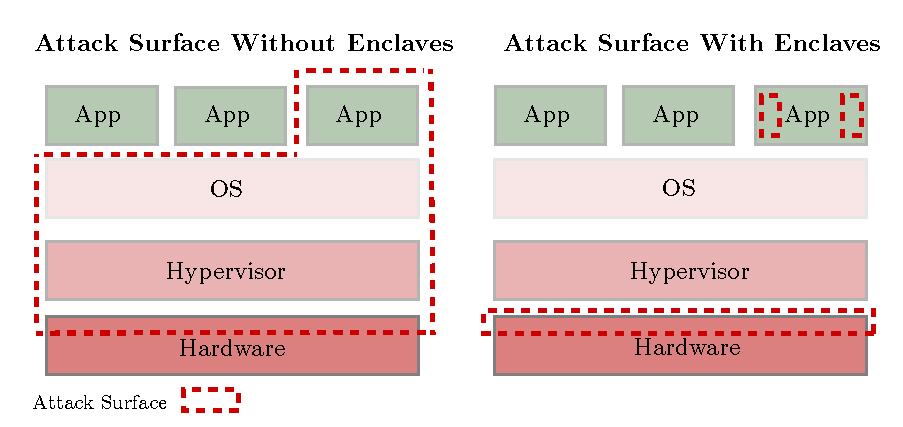
\includegraphics[width=\textwidth]{enclave}
	\caption[Attack surface with \acrshort{tee}]{
		Attack surface with \acrshort{tee}.
		Adapted from \url{sgx101.gitbook.io}.
	}%
	\label{figure:enclave}
\end{figure}


		While \acrshort{tee} is a concept defining an execution environment, specific solutions include a hardware security module (a plug-in device with a protected memory and a crypto-optimized processing unit), an \acrshort{fpga}, and a set of extensions to an existing processor architecture, such as an \acrshort{sgx} for Intel x86 or Secure Encrypted Virtualization \cite{amd-memory-encryption} for AMD\@.
		Of all these, Intel \acrshort{sgx} is the most widely used technology.

		\subsection{\texorpdfstring{\acrlong{sgx}}{Software Guard Extensions}}

			\acrfull{sgx} is a set of instructions for the Intel x86 architecture that allow a user or an \acrlong{os} to define a region of protected memory, called the \emph{enclave}, and interact with it.
			The enclave can only be accessed using the \acrshort{sgx} instructions (i.e, regular \texttt{mov} instruction would not work), and all pages of the enclave are symmetrically encrypted and physically protected.
			\acrshort{sgx} guarantees the integrity and security of the memory pages within the enclave.
			Although the size of enclave memory is very limited, \acrshort{sgx} can use regular \acrshort{ram} by transparently swapping the pages between the trusted and untrusted memory.
			The pages are then encrypted with integrity protection when placed in the \acrshort{ram} (\emph{sealing} in \acrshort{sgx} terms).

			An \acrshort{sgx}-enabled application declares its trusted and untrusted components upfront.
			Trusted part will live entirely in the enclave, while the untrusted part is a normal process that runs within the \acrshort{os}.
			The application has to be digitally signed for the enclave to accept it, and the enclave itself can authenticate to the user via an \emph{attestation} process.
			Conceptually, the simplest \acrshort{sgx} application in an outsourced database system can be seen as a trusted component that operates over sensitive material (e.g., keys, tokens, plaintext user data), a remote trusted client application that communicates with the enclave, and a layer of code that passes requests through (untrusted part of an \acrshort{sgx} application).
			Cipherbase \cite{cipherbase-daas} and StealthDB \cite{stealth-db} are good examples of such approach.

		\subsection{Issues with \acrshort{sgx}}

			\acrshort{sgx}, as the closest instantiation of \acrshort{tee} available, has been extensively targeted.
			The attacks include Foreshadow \cite{foreshadow}, Prime+Probe cache attack \cite{prime-probe-sgx-attack}, an attack from within the enclave \cite{enclave-sgx-attack}, Spectre line of attacks that can bypass \acrshort{sgx} \cite{spectre-sgx-attack}, replay attack \cite{replay-sgx-attack}, Plundervolt attack \cite{plundervolt-sgx-attack}, Load Value Injection attack \cite{lvi-sgx-attack} and SGAxe attack \cite{sgaxe-sgx-attack}.
			Due to its many security issues, \acrshort{sgx} has been officially discontinued.\footnote{As of $11^\text{th}$ Generation Intel Core processor.}

			Besides the attacks against the \acrshort{sgx}, the design itself has a number of restrictions.
			First of all, the enclave memory is capped at \SI{128}{\mega\byte}, part of which is occupied by the \acrshort{sgx} control structures, leaving the application about \SI{96}{\mega\byte}.
			\acrshort{sgx} allows the use of external memory pages through the sealing mechanism, but it imposes high overhead of re-encryption and crossing the enclave physical boundary.
			Second, the code execution inside the enclave is significantly slower.
			Third, by design, only the untrusted application component can interact with the \acrshort{os}, for example, make network or storage \acrshort{io} requests.
			Finally, from the security standpoint the enclave is vulnerable against the side-channel attacks, most of all, access pattern leakage.
			Such leakage implies that the normal database application cannot be placed directly in the enclave and be deemed secure, because access pattern has been effectively exploited up to a reconstruction attack \cite{generic-attacks-kellaris}.
			One then has to design the application specifically to conceal the access pattern.
			For example, ZeroTrace \cite{zerotrace} is a variant of PathORAM \cite{path-oram} that is internally oblivious and thus can work in \acrshort{sgx}.
			Oblix \cite{oblix} is another example of a structure that is, in \textcite{oblix} own terms, doubly-oblivious --- internally in how manages memory and registers, and externally in how it interacts with a storage.

	\cleardoublepage%
	\chapter{Related work}
\thispagestyle{myheadings}

	\section{Privacy}

		\subsection{$k$-anonymity}

		\subsection{$l$-diversity}

		\subsection{$t$-closeness}

		\subsection{\acrlong{dp}}

	\section{Range query security in a snapshot model}

		\subsection{Property-preserving encryption}

		\subsection{Searchable symmetric encryption}

		\subsection{Fully homomorphic encryption}

		\subsection{Attacks}

	\section{Range query security in a persistent model}

		\subsection{Access pattern}

		\subsection{Communication volume}

		\subsection{Secure Enclave}

		\subsection{Attacks}

	\section{\acrshort{knn} query security in a snapshot model}

		\subsection{Attacks}

	\cleardoublepage%
	\chapter{Range queries in the snapshot model}
\thispagestyle{myheadings}

	In this section\ldots{}

	\chapter{Introduction}\label{section:introduction}

\thispagestyle{myheadings}

	\section{A few remarks before you start}\label{section:introduction:history}

		Intro goes here  \Gls{ad}.
		And one reference~\cite{practical-ore}.

		\begin{figure}[hb]
	\centering
	
\includegraphics[width=0.33\textwidth]{goethe}
	\caption[Short caption]{
		Long caption.
		Multiline.
	}\label{figure:goethe}
\end{figure}


		Reference to \cref{figure:goethe}.

		And one \href{https://dbogatov.org}{link}.


	\section{Security Perspective}\label{sec:security}

	Each scheme and protocol we analyze has its own security definition, which captures different leakage levels.
	We attempt to unify these definitions and analyze them under a common framework.
	We also attempt to assess relative security of these definitions and analyze their leakages.

	In this work we mostly consider the snapshot model, where the attacker can observe all the database contents at one time instant.
	Note that this excludes timing attacks such as measuring encryption time.
	All security definitions of the schemes and protocols that we discuss here are based on this model.
	Also, the snapshot attacker is the most common attacker that we face today~\cite{secure-queries-overview}.
	The idea is that a hacker or an insider can steal the entire encrypted database and all its contents at some point in time.

	Beyond the snapshot model, it is also possible to consider a stronger adversary who can track communication volume and data access patterns in real time.
	Approaches that help protect against such an attacker include ORAM for protection against access pattern leakage and differential privacy for protection against communication volume leakage.
	Although this model is not a primary target of this paper, our benchmark includes a protocol (Section~\ref{sec:oram}) that is secure in this setting to show the cost of adding such protection.

	We wanted to specifically comment on a work of \textcite{leakage-abuse-grubs-2017}, which demonstrates a series of attacks against OPE and ORE schemes.
	The attacks can be very successful, but they depend on certain prerequisites.
	First, all attacks assume the existence of a well-correlated auxiliary dataset.
	Second, the binomial attack, which works against a ``perfectly secure frequency-hiding scheme'', reliably recovers only high-frequency elements.
	Finally, the attacks are specifically devastating against encrypted strings (e.g.\ first and last names) as opposed to numerical data, and we also do not recommend using OPE / ORE for strings (see Section~\ref{sec:variable-inputs}).
	One of the conclusions of our work is that security is negatively correlated with performance and it is up to a practitioner to trade off security and performance constraints.

	\subsection{A note on variable-length inputs}\label{sec:variable-inputs}

		A generic OPE / ORE scheme accepts bit-strings of any length as inputs, and treats them as numbers or processes them bit-by-bit.
		We warn against supplying raw bytes of variable length (e.g.\ encoded strings) to OPE and ORE schemes, as such an approach will introduce both performance and security challenges.

		From the performance standpoint, the complexity of OPE / ORE schemes usually depends on the input length at least linearly (see Table~\ref{tbl:primitive-usage-theory}).
		32-bit numbers already introduce a noticeable overhead for some (usually more secure) schemes, and supplying arbitrary-length inputs may worsen performance by at least an order of magnitude.

		Security of such a construction will be minimal as most schemes leak some information about the magnitude of the difference, and longer inputs will naturally be treated as larger numbers.
		Thus, the difference between long and short inputs will be apparent.
		We refer to the work of~\textcite{leakage-abuse-grubs-2017} as they have a practically supported discussion of security consequences of using OPE / ORE with arbitrary strings.

		On the other hand, other protocols in our benchmark can usually handle variable-length inputs as long as they fit into a single block for the underlying block cipher.


	\section{\texorpdfstring{\acrshort{ope}}{OPE} and \texorpdfstring{\acrshort{ore}}{ORE} Schemes}

	An \acrlong{ore} scheme is a triple of polynomial\hyp{}time algorithms $\setup$, $\encrypt$ and $\compare$.
	$\setup$ generates a key of parameterized length (the $\lambda$ parameter).
	$\encrypt$ takes a numerical input (as a bit string) and produces a ciphertext.
	$\compare$ takes two ciphertexts generated by the scheme and outputs whether the first plaintext was strictly less than the second.
	Note that being able to check this condition is enough to apply all other comparison operators ($<$, $\le$, $=$, $\ge$, $>$).
	Also note that an \acrshort{ore} scheme does not include a decryption algorithm, because one can simply append a symmetric encryption of the plaintext to the produced ciphertext and use it for decryption.\footnote{
		\emph{Given the secret key}, it is possible to decrypt a ciphertext by doing binary search on the plaintext domain: encrypting known values and comparing them against the target ciphertext, until the target plaintext is found.
		However, this would require $\bigO{\log{|\domain|}}$ encryption and comparison operations.
	}
	An \acrfull{ope} scheme is a particular case of an \acrshort{ore} scheme where ciphertexts are numerical and thus $\compare$ routine is trivial (the numerical order of ciphertexts is the same as underlying plaintexts).
	\acrshort{ope} may optionally include a decryption algorithm, since appending a symmetric ciphertext is no longer possible.

	Both \acrshort{ope} and \acrshort{ore} schemes by definition allow to totally order the ciphertexts.
	This is their inherent leakage (by design) and all the \acrshort{ope} / \acrshort{ore} security definitions account for this and possibly additional leakage.

	We proceed by describing and analyzing the \acrshort{ope} / \acrshort{ore} schemes we have benchmarked.
	All plaintexts are assumed to be 32-bit signed integers, or $n$-bit inputs in complexity analysis.
	\acrshort{ope} ciphertexts are assumed to be 64-bit signed integers.

	From here, we will use the term \acrshort{ore} to refer to both \acrshort{ope} and \acrshort{ore}, unless explicitly stated otherwise.
	Each scheme has its own subsection where the first part is the construction overview followed by security discussion, and the second part is our theoretical and experimental analysis.

	\subsection{BCLO OPE}

	The OPE scheme by \textcite{bclo-ope} was the first OPE scheme that provided formal security guarantees and was used in one of the first database systems that executes queries over encrypted data (CryptDB \cite{crypt-db}).
 	The core principle of their construction is the natural connection between a random order-preserving function and the hypergeometric probability distribution.

	The encryption algorithm works by splitting the domain into two parts according to a value sampled from the hypergeometric distribution ($\hg$) routine, and splitting the range in half recursively.
	When the domain size contains a single element, the corresponding ciphertext is sampled uniformly from the current range.

	All pseudo-random decisions are made by an internal PRG ($\tapegen$ in \cite{bclo-ope}).
	This way not only the algorithm is deterministic, but also decryption is possible.
	The decryption procedure takes the same ``path'' of splitting domain and range, and when the domain size reaches one, the only value left is the original plaintext.

	\subsubsection{Security}
		This scheme is POPF-CCA secure \cite{bclo-ope}, meaning that it is as secure as the underlying ideal object --- randomly sampled order-preserving function from a certain domain to a certain range.
		For practical values of the parameters, \textcite{ope-leakage} showed that the distance between the plaintexts can be approximated to an accuracy of about the square root of the domain size.
		In other words, approximately, half of the bits (the most significant) are leaked.
		\textcite{leakage-abuse-grubs-2017} showed that this leakage allows to almost entirely decrypt the ciphertexts (given auxiliary data with a similar distribution) and encrypting strings (rather than numbers) with this scheme is especially dangerous (see \cref{section:range-snapshot:variable-inputs}).

	\subsubsection{Analysis and implementation challenges}

		Efficient sampling from the hypergeometric distribution is a challenge by itself.
		Authors suggest using a randomized yet exact (not approximate) Fortran algorithm by \textcite{hg-sampler}.
		It should be noted that the algorithm relies on infinite precision floating-point numbers, which most regular frameworks do not have.
		The security consequences of finite precision computations is actually an open question.
		The complexity of this randomized algorithm is hard to analyze; however, we empirically verified that its running time is no worse than linear in the input bit length.
		The authors also suggest a different algorithm for smaller inputs \cite{hg-sampler-small}.

		On average, encryption and decryption algorithms make $n$ calls to $\hg$, which in turn consumes entropy generated by the internal PRG\@.
		The entropy, and thus the number of calls to PRG, needed for one $\hg$ run is hard to analyze theoretically.
		However, we derived this number experimentally (see \cref{section:range-snapshot:evaluation}).

		BCLO has been implemented in numerous languages and has been deployed in a number of secure systems.
		We add {\Csharp} implementation to the list, and recommend using a library that supports infinite precision floating-point numbers when building the hypergeometric sampler.


	\subsection{CLWW \acrshort{ore}}\label{section:range-snapshot:clww}

	The \acrshort{ore} scheme by \textcite{clww-ore}, which authors call ``Practical ORE'', is the first efficient \acrshort{ore} implementation based on \acrshortpl{prf}.

	On encryption, the plaintext is split into $n$ values in the following way.
	For each bit, a value is this bit concatenated with all more significant bits.
	This value is given to a keyed \acrshort{prf} and the result is numerically added to the next less significant bit.
	This resulting list of $n$ elements is the ciphertext.

	The comparison routine traverses two lists in-order looking for the case when one value is greater than the other by exactly one, revealing location and value of the first differing bit.
	If no such index exists, the plaintexts are equal.

	\subsubsection{Security}
		A generic \acrshort{ore} security definition was introduced along with the scheme \cite{clww-ore}.
		\acrshort{ore} leakage is more clearly quantified than in \acrshort{ope}.
		The definition says that the scheme is secure with a leakage $\leak(\cdot)$ if there exists an algorithm (simulator) that has access to the leakage function and can generate output indistinguishable from the one generated by the real scheme.
		This scheme satisfies \acrshort{ore} security definition with the leakage $\leak(\cdot)$ of the location and value of the first differing bit of every pair of plaintexts.
		Note that the most significant differing bit also leaks the approximate distance between two values.

	\subsubsection{Analysis and implementation challenges}

		On encryption the algorithm makes $n$ calls to \acrshort{prf} and the comparison procedure does not use any cryptographic primitives.
		Ciphertext is a list of length $n$, where each element is an output of a \acrshort{prf} modulo 3.
		The authors claim that the ciphertext's size is $n \log_2 3$, just $1.6$ times larger than the plaintext's size.
		While this may be true for large enough $n$ if ternary encoding is used, we found that in practice the ciphertext size is still $2n$.
		$1.6 n$ for 32-bit words is $51.2$ bits, which will have to occupy one 64-bit word, or two 32-bit words, therefore resulting in $2n$ anyway.


	\subsection{Lewi-Wu ORE}

	\textcite{lewi-wu-ore} presented an improved version of the CLWW scheme~\cite{clww-ore} which leaks strictly less.

	The novel idea was to use the ``left / right framework'' in which two ciphertexts get generated --- left and right.
	The right ciphertexts are semantically secure, so an adversary will learn nothing from them.
	Comparison is only defined between the left ciphertext of one plaintext and the right ciphertext of another plaintext.

	The approach is to split the plaintext into blocks of $d$ bits.
	The ciphertext is computed block-wise.
	For the right side, the algorithm compares the given block value to all $2^d$ possible block values; each comparison result is added (modulo 3) to a PRF of the previous blocks.
	All $2^d$ comparison results go into the right ciphertext.
	The left side, which is shorter, is produced in such a way as to reveal the correct comparison result.
	This way the location of the differing bit inside the block is hidden, but the location of the first differing block is revealed.

	\subsubsection{Security}
		This scheme satisfies the ORE security definition introduced by~\textcite{clww-ore} with the leakage $\leak(\cdot)$ of the location of the first differing \emph{block}.
		This property allows a practitioner to set performance-security tradeoff by tuning the block size.
		Left / right framework is particularly useful in a {\BPlus} tree since it is possible to store only one (semantically secure) side of a ciphertext in the structure (see Section~\ref{sec:ore-to-protocol}).

	\subsubsection{Analysis and implementation challenges}

		Let $n$ be the size of input in bits (e.g.\ 32) and $d$ be the number of bits per block (e.g.\ 2).

		Left encryption loops $\frac{n}{d}$ times making one PRP call and two PRF calls each iteration.
		Right encryption loops $\frac{n}{d} 2^d$ times making one PRP call, one hash call and two PRF calls each iteration.
		Comparison makes $\frac{n}{d}$ calls to hash at worst and half of that number on average.
		Please note that the complexity of right encryption is exponential in the block size.
		In the Table~\ref{tbl:primitive-usage-theory} the PRP usage is linear due to our improvement.
		The ciphertext size is no longer negligible --- $\frac{n}{d} \left(\lambda + n + 2^{d + 1} \right) + \lambda$, for $\lambda$ being PRF output size.

		The implementation details of this approach raise an interesting security question.
		Although the authors suggest using 3-rounds Feistel networks~\cite{unbalanced-feistel} for PRP and use it in their implementation, it may not be secure for small input sizes.
		Feistel networks security depends on the input size~\cite{feistel-security} --- exponential in the input size.
		However, the typical input for PRP in their scheme is 2--8 bits, thus even exponential number is small.

		We have considered multiple PRP implementations to use instead of the Feistel networks.
		Because the domain size is small (from $2^2$ to $2^8$ elements), we have decided to build a PRP by simply using the key as an index into the space of all possible permutations on the domain, where a permutation is obtained from the key via Knuth shuffle (this approach was mentioned in~\cite{knuth-shuffle-security}).
		Another important aspect of the implementation is that for each block we need to compute the permutation of all the values inside the block.
		This operation applied many times can be expensive.
		To address this, we propose to generate a PRP table once for the whole block and then use this table when one needs to compute the location of an element of permutation.
		This can reduce the PRP usage (indeed, we observe a reduction from 80 to 32 calls in our case).
		We evaluate this improved approach in our experimental section.


	\subsection{CLOZ ORE}

	\textcite{parameter-hiding-ore} introduced a new ORE scheme that provably leaks less than any previous scheme.
	The idea is to use \textcite{clww-ore} construction (see Section~\ref{sec:clww}), but permute the list of PRF outputs.
	The original order of those outputs is not necessary, as one can simply find a pair that differs by one.
	This is not enough to reduce leakage, however, since an adversary can count how many elements two ciphertexts have in common.

	To address this problem, the authors define a new primitive they call a \emph{property-preserving hash} (PPH).
	A PPH as defined and used in~\cite{parameter-hiding-ore}, allows one to expose a property (specifically $y \overset{?}{=} x + 1$) of two (numerical) elements such that nothing else is leaked.
	In particular, the outputs are randomized, so same element hashed twice will have different hashes.
	Please refer to the original paper~\cite{parameter-hiding-ore} for formal correctness and security definitions.

	Equipped with the PPH primitive, the algorithm ``hashes'' the elements of the ciphertexts before outputting them.
	Due to security of PPH, the adversary would not be able to count how many elements two ciphertexts have in common, thus, would not be able to tell the location of differing bit.

	\subsubsection{Security}
		The strong side of the scheme is its security.
		The scheme leaks $\leak(\cdot)$ an \emph{equality pattern} of the most-significant differing bits (satisfying \textcite{clww-ore} definition).
		As defined in \cite{parameter-hiding-ore}, the intuition behind equality pattern is that for any triple of plaintexts $m_1$, $m_2$, $m_3$, it leaks whether $m_2$ differs from $m_1$ before $m_3$ does. % chktex 2
		We do not know of any attacks against this construction (partially because no implementation exists yet, see next subsection), but it is inherently vulnerable to frequency attacks that apply to all frequency-revealing ORE schemes (see Section~\ref{sec:security}).

	\subsubsection{Analysis and implementation challenges}

		On encryption, the scheme makes $n$ calls to PRF, $n$ calls to PPH \textsc{Hash} and one call to PRP\@.
		Comparison is more expensive, as the scheme makes $n^2$ calls to PPH \textsc{Test}.

		The scheme has two limitations that make it impractical.
		The first one is the square number of calls to PPH, which is around $1024$ for a single comparison.

		The second problem is the PPH itself.
		Authors suggest a construction based on bilinear maps.
		The hash of an argument is an element of a group, and the test algorithm is computing a pairing.
		This operation is very expensive --- order of magnitude more expensive than any other primitive we have implemented for other schemes.

		We have implemented this scheme in C++ using the PBC library~\cite{pbc} to empirically assess schemes's performance, and on our machine (see Section~\ref{sec:evaluation}), a single comparison takes 1.9 seconds on average.
		Although we have produced the first (correct and secure) real implementation of this scheme in C++, it is infeasible to use it in the benchmark (it will take years to complete a single run).
		Therefore, for the purposes of our benchmark, we implemented a ``fake'' version of PPH --- correct, but insecure, which does not use pairings.
		Consequently, in our analysis we did not benchmark the speed of the scheme, but measured all other data.


	\subsection{FH-OPE}

	Frequency-hiding OPE by \textcite{fh-ope} is a stateful scheme that hides the frequency of the plaintexts, so the adversary is unable to construct a frequency histogram.

	This scheme is stateful, which means that the client needs to keep a data structure and update it with every encryption and decryption.
	The data structure is a binary search tree where the node's value is the plaintext and node's position in a tree is the ciphertext.
	For example, consider the range $[1, 128]$.
	Any plaintext that happens to arrive first (for example, $6$), will be the root, and thus the ciphertext is $64$.
	Then any plaintext smaller than the root, say $3$, will become the left child of the root, and will produce the ciphertext $32$.
	To encrypt a value, the algorithm traverses the tree until it finds a spot for the new plaintext, or finds the same plaintext.
	If the same plaintext is found, the traversal pseudo-randomly passes to the left or right child, up to the leaf.
	This way, the invariant of the tree --- intervals of the same plaintexts do not overlap --- is maintained.
	The ciphertext generated from the new node's position is returned.

	Due to randomized ciphertexts, the comparison algorithm is more complicated than in the regular deterministic OPE\@.
	To properly compare ciphertexts, the algorithm needs to know the boundaries --- the minimum and maximum ciphertexts for a particular plaintext.
	The client is responsible for traversing the tree to find the plaintext for the ciphertext and then minimum and maximum ciphertext values.
	Having these values, the comparison is trivial --- equality is a check that the value is within the boundaries, and other comparison operators are similar.

	Authors have designed a number of heuristics to minimize the state size, however, these are mostly about compacting the tree and the result depends highly on the tree content.
	In our analysis, we consider the worst case performance without the use of heuristics.
	In our experimental evaluation, however, we did implement compaction.

	\subsubsection{Security}
		The security of the scheme relies on the large range size to domain size ratio.
		Authors recommend at least 6 times longer ciphertexts than the plaintexts in bit-length, which means ciphertexts should be 192-bit numbers that are not commonly supported.
		It is possible to operate over arbitrary-length numbers, but the performance overhead would be substantial.
		We did a quick micro-benchmark in {\Csharp} and the overhead of using \texttt{BigInteger} is 15--20 times for basic arithmetic operations.

		This scheme satisfies IND-FAOCPA definition (introduced along with the scheme~\cite{fh-ope}), meaning that it does not leak the equality or relative distance between the plaintexts.
		This definition has been criticized in~\cite{florian-def-critique}, who claim that the definition is imprecise and propose an enhanced definition along with a small change to construction to satisfy this new definition.
		Both schemes leak the insertion order, because it affects the tree structure.
		We do not know of any attacks against this leakage, but it does not mean they cannot exist.
		\textcite{leakage-abuse-grubs-2017} describe an attack against this scheme (binomial attack), but it applies to any perfectly secure (leaking only total order) frequency-hiding OPE\@.

	\subsubsection{Analysis and implementation challenges}

		If the binary tree grows in only one direction, at some point it will be impossible to generate another ciphertext.
		In this case, the tree has to be rebalanced.
		This procedure will invalidate all ciphertexts already generated.
		This property makes the scheme difficult to use in some protocols since they usually rely on the ciphertexts on the server being always valid.
		The authors explicitly mention that the scheme works under the assumption of uniform input.
		However, the rebalancing will be caused by insertion of just 65 consecutive input elements for 64-bit integer range.

		The scheme makes one tree traversal on encryption and decryption.
		Comparison is trickier as it requires one traversal to get the plaintext, and two traversals for minimum and maximum ciphertexts.
		We understand that it is possible to get these values in fewer than three traversals, but we did not optimize the scheme for the analysis and evaluation.

		For practitioners we note that the stateful nature of the scheme implies that the client storage is no longer negligible as the state grows proportionally to the number of encryptions.
		We also note that implementing compaction extensions will affect code complexity and performance.
		Finally, we stress again that some non-uniform inputs can break the scheme by causing all ciphertexts to be invalid.
		It is up to the users of the scheme to ensure uniformity of the input, which poses serious restrictions on the usage of the scheme.


	% cSpell:ignore Lewi BCLO CLWW captionsetup

\begin{sidewaystable}
	\renewcommand{\arraystretch}{1.5}
	\centering
	\captionsetup{width=\textwidth}
	\caption[Primitive usage by \acrshort{ope} / \acrshort{ore} schemes]{
		\cite[Tables 1 and 4]{ore-benchmark-17}.
		Primitive usage by \acrshort{ope} / \acrshort{ore} schemes.
		Ordered by security rank --- most secure below.
		$n$ is the input length in bits, $d$ is a block size for Lewi-Wu \cite{lewi-wu-ore} scheme, $\lambda$ is a \acrshort{prf} output size, $N$ is a total data size, \textbf{\acrshort{hg}} is a hyper-geometric distribution sampler, \textbf{\acrshort{pph}} is a property-preserving hash with $h$-bit outputs built with bilinear maps and \textbf{bolded} are weak points of the schemes.
		Values in parentheses are simulation-derived. $N = 10^3$, $n = 32$, $d = 2$, $\lambda = 128$ and $h = 128$ in this simulation.
	}\label{tbl:primitive-usage-theory}
	\begin{tabular*}{\linewidth}{ !{\extracolsep\fill} l c c c c c } % chktex 26

		\toprule

		\multirow{2}{*}{Scheme}						& \multicolumn{2}{c}{Primitive usage (number of invocations)}																				& \multirow{2}{*}{\makecell{Ciphertext size, \\ or state size (bits)}}					&  \multirow{2}{*}{\makecell{Leakage \\ (in addition to inherent total order)}}				\\ \cline{2-3}
		\rule{0pt}{10pt}							& Encryption																& Comparison													& 																						& 																							\\

		\toprule

		\cite{bclo-ope}								& $\bm{\approx n}$ \textbf{(41) \acrshort{hg}}								& none															& $2n$ (64)																				& \textbf{$\approx$ Top half of the bits}													\\

		\midrule

		\cite{clww-ore}								& $n$ (32) \acrshort{prf} 													& none															& $2n$ (64)																				& \textbf{Most-significant differing bit}													\\

		\midrule

		\multirow{3}{*}{\cite{lewi-wu-ore}}			& \boldmath{} $\nicefrac{2n}{d}$ \unboldmath{} \textbf{(32) \acrshort{prp}}	& \multirow{3}{*}{$\frac{n}{2d}$ (9) Hash}						& 																						& \multirow{3}{*}{Most-significant differing block}											\\
													& $2 \frac{n}{d} \left( 2^d + 1 \right)$ (160) \acrshort{prf}				&																& $\frac{n}{d} \left(\lambda + n + 2^{d + 1} \right) + \lambda$							&																							\\
													& $\frac{n}{d} 2^d$ (64) Hash												&																& (2816)																				&																							\\


		\midrule

		\multirow{3}{*}{\cite{parameter-hiding-ore}}			& $n$ (32) \acrshort{prf}													& \multirow{3}{*}{$\bm{n^2}$ \textbf{(1046) \acrshort{pph}}}	& \multirow{3}{*}{$n \cdot h$ (4096)}													& \multirow{3}{*}{\makecell{Equality pattern \\ of the most-significant \\ differing bit}}	\\
													& $n$ (32) \acrshort{pph}													&																&																						& 																							\\
													& 1 \acrshort{prp}															&																&																						& 																							\\

		\midrule

		\cite{fh-ope}								& 1 Traversal																& 3 Traversals													& $\bm{3 \cdot n \cdot N}$ \textbf{(86842)}												& Insertion order																			\\

		\bottomrule

	\end{tabular*}
\end{sidewaystable}


\section{Secure Range Query Protocols}

	We proceed by describing and analyzing the range query protocols we have chosen.
	For the purpose of this paper, a secure range-query protocol is defined as a client-server communication involving construction and search stages.
	Communication occurs between a client, who owns some sensitive data, and an honest server, who securely stores it.
	In construction stage, a client sends the server the encrypted datapoints (index-value tuples) and the server stores them in some internal data structure.
	In search stage, a client asks the server for a range (usually specifying it with encrypted endpoints) and the server returns a set of encrypted records matching the query.
	Note that the server may interact with the client during both stages (e.g.\ ask the client to sort a small list of ciphertexts).
	Also note that we do not allow batch insertions as it would limit the use cases (e.g.\ client may require interactive one-by-one insertions).

	The first protocol is a family of constructions where a data structure ({\BPlus} tree in this case) uses \acrshort{ore} schemes internally.
	Then, we present alternative solutions with varying performance and security profiles, not relying on \acrshort{ore}.
	Finally, we introduce two baseline solutions we will use in the benchmark --- one that achieves the best performance and the other that achieves the maximal security.

	\subsection{Range query protocol from \texorpdfstring{\acrshort{ore}}{ORE}}\label{section:range-snapshot:ore-to-protocol}

	So far we have analyzed \acrshort{ope} and \acrshort{ore} schemes without much context.
	One of the best uses of an \acrshort{ore} is within a secure protocol.
	In this section we provide a construction of a search protocol built with a {\BPlus} tree working on top of an \acrshort{ore} scheme and analyze its security and performance.

	The general idea is to consider some data structure that is optimized for range queries, and to modify it to change all comparison operators to \acrshort{ore} scheme's $\compare$ calls.
	This way the data structure can operate only on ciphertexts.
	Performance overhead would be that of using the \acrshort{ore} scheme's $\compare$ routine instead of a plain comparison.
	Space overhead would be that of storing ciphertexts instead of plaintexts.

	In this paper, we have implemented a typical {\BPlus} tree \cite{b-tree} (with a proper deletion algorithm \cite{b-plus-tree-deletion}) as a data structure.

	For protocols, we also analyze the \acrshort{io} performance and the communication cost.
	In particular, we are interested in the expected number of \acrshort{io} requests the server would have made to the secondary storage, and the number and size of messages parties would have exchanged.

	The relative performance of the {\BPlus} tree depends only on the page capacity (the longer the ciphertexts, the smaller the branching factor). 	Therefore, the query complexity is $\bigO{\log_B \left( \nicefrac{N}{B} \right) + \nicefrac{r}{B}}$, where $B$ is the number of records (ciphertexts) in a block, $N$ is the number of records (ciphertexts) in the tree and $r$ is the number of records (ciphertexts) in the result (none for insertions).

	Communication amount of the protocol is relatively small as its insertions and queries require at most one round trip.

	\subsubsection{Security}
		The leakage of this protocol consists of leakage of the underlying \acrshort{ore} scheme plus whatever information about insertion order is available in the {\BPlus} tree.
		Please note that Lewi-Wu \cite{lewi-wu-ore} \acrshort{ore} is particularly well-suited in this construction with its left / right framework, because only the semantically secure side of the ciphertext is stored in the structure.
		In this case, the \acrshort{ore} leakage becomes only the total order and the security of the protocol is comparable with other non-\acrshort{ore} constructions.


	\subsection{Kerschbaum-Tueno}

	\textcite{florian-protocol} proposed a new data structure, which satisfies their own definitions of security (IND-CPA-DS) and efficiency (search operation has poly\hyp{}logarithmic running time and linear space complexity).

	In short, the idea is to maintain a (circular) array of symmetrically encrypted ciphertexts in order.
	On insertion, the array is rotated around a uniformly sampled offset to hide the location of the smallest element.
	Client interactively performs a binary search requesting an element, decrypting it and deciding which way to go.

	\subsubsection{Security}
		Authors prove that this construction is IND-CPA-DS secure (defined in the same paper \cite{florian-protocol}).
		The definition assumes an array data structure and therefore serves specifically this construction (as opposed to being generic).
		It provably hides the frequency due to semantic encryption and hides the location of the first element due to random rotations.
		Leakage-wise this construction is strictly better than {\BPlus} tree with ORE --- they both leak total order, but \cite{florian-protocol} hides distance information and smallest / largest elements.
		Specifically, for all pairs of consecutive elements $e_i$ and $e_{i+1}$ it is revealed that $e_{i+1} \ge e_i$ except for one pair of smallest and largest elements in the set.

	\subsubsection{Analysis and implementation challenges}

		Insertions are {\IO}-heavy because they involve rotation of the whole data structure.
		All records will be read and written, thus the complexity is $\bigO{\nicefrac{N}{B}}$.
		Searches are faster since they involve logarithmic number of blocks.
		The first few blocks can be cached and the last substantial number of requests during the binary search will target a small number of blocks.
		The complexity is then $\bigO{\log_2 \nicefrac{N}{B}}$.

		Communication volume is small as well.
		Insertion requires $\log_2 N$ messages from each side.
		Searches require double that number because separate protocol is run for both endpoints.

		The data structure is linear in size, and the client storage is always small.
		Sizes of messages are also small as only a single ciphertext is usually transferred.

		For practitioners we have a few points.
		The construction in the original paper \cite{florian-protocol} contains a typo as $m$ and $m^\prime$ must be swapped in the insertion algorithm.
		Also, we have found some rare edge cases; when duplicate elements span over the modulo, the algorithm may not return the correct answer.
		Both inconsistencies can be fixed however.
		This protocol is not optimized for {\IO} operations for insertions, and thus would be better suited for batch uploads.


	\subsection{POPE}

	\textcite{pope} presented a protocol, direct improvement over mOPE \cite{ope-ideal-security-protocol}, which is especially suitable for large number of insertions and small number of queries.
	The construction is heavily based on buffer trees \cite{buffer-tree} to support fast insertion and lazy sorting.

	The idea is to maintain a POPE tree on the server and have the client manipulate that tree.
	POPE tree is similar to B-tree, in that the nodes have multiple children and nodes are sorted on each level.
	Each node has an ordered list of \emph{labels} of size $L$ and an unbounded unsorted set of encrypted data called buffer.
	Parameter $L$ controls the list size, the leaf's buffer size, and the size of client's working set.
	The insertion procedure simply adds an encrypted piece of data to the root's buffer, thus we do not concentrate on insertion analysis in this section.

	The query procedure is more complex.
	To answer a query, the server interacts with the client to split the tree according to the query endpoints.
	On a high level, for each endpoint the buffers are cleared (content pushed down to leaves), and nodes in the paths are split.
	After that, answering a query means replying with all ciphertexts in all buffers between the two endpoint leaves.

	The authors provide cost analysis of their construction.
	Search operations are expected to require $\bigO{\log_L n}$ rounds.
	It must be noted that the first queries will require many more rounds, since large buffers must be sorted.

	\subsubsection{Security}
		This construction satisfies the security definition of frequency\hyp{}hiding partial order-preserving (FH-POP) protocol (introduced in the paper \cite{pope}).
		According to \cite[Theorem~3]{pope}, after $n$ insertions and $m$ queries with local storage of size $L$, where $m L \in o(n)$, the POPE scheme is frequency-hiding partial order-preserving with $\bigOmega{ \frac{n^2}{mL \log_L n} - n }$ incomparable pairs of elements. % chktex 2
		Simply put, the construction leaks pairwise order of a \emph{bounded} number of elements.
		Aside from this, the construction provably hides the frequency (i.e.\ equality) of the elements.

	\subsubsection{Analysis and implementation challenges}

		In our analysis we count each request-response communication as a round.
		This is different from \cite{pope} where they use \emph{streaming} a number of elements as a single round. % chktex 2
		The rationale for our approach is that if we allow persistent channels additionally to messages, then any protocol can open a channel for each operation.
		Thus, we do not allow channels for all protocols in our analysis.

		Also, as noted by the authors, if $L = n^{\epsilon}$ for $0 < \epsilon < 1$, then the amortized costs become $\bigO{1}$.
		While this is true, in our analysis the choice of $L$ depends on the storage volume block size for {\IO} optimizations, instead of the client's volatile storage capacity.
		Thus, the costs remain logarithmic.

		Search bandwidth depends heavily on the current state of the tree.
		When the tree is completely unsorted (the first query), all elements of the tree will be transferred to split the large root, then possibly internal node will have to be split requiring sending of $\frac{N}{L}$ elements, and so on, thus $\bigO{N + r}$.
		When the tree is completely sorted (after a large number of uniform queries), the bandwidth will be similar to that of a standard {\BPlus} tree --- $\bigO{L \log_L N + r}$.
		The average case is hard to compute; however, authors prove an upper bound on bandwidth after $n$ insertions and $m$ queries --- $\bigO{m L \log_L n + n \log_L m + n \log_L (\lg n) }$.

		POPE tree is not optimized for {\IO} the way B-tree is.
		Search complexity is hard to analyze as is bandwidth complexity.
		In the worst-case (first query), all blocks need to be accessed $\bigO{\frac{N}{B} + \frac{r}{B}}$.
		In the best-case all nodes occupy exactly one block and {\IO} complexity is the same as with {\BPlus} tree $\bigO{\log_L \frac{N}{B} + \frac{r}{B}}$.
		The average case is in between and matters get worse as the node is not guaranteed to occupy a single block due to the buffers of arbitrary size.

		Client's persistent storage is negligibly small --- it stores the encryption key.
		Volatile storage is bounded by $L$.

		For practitioners we present a number of things to consider.
		Buffer within one node is unsorted, so in the worst-case, $L$-sized chunks remain unordered.
		Due to this property, the query result may contain up to $2 (L - 1)$ extra entries, which the client will have to discard from the response.

		The first query after a large number of insertions will result in client sorting the whole $N$ elements, and thus, POPE has different performance for cold and warm start.
		Also, even to navigate an already structured tree, the server has to send to the client the whole $L$ elements and ask where to go on all levels.

		Furthermore, \cite{pope} does not stress the fact that after alternating insertions and queries, it may happen that some intermediate buffers are not empty, thus returning buffers between endpoints must include intermediate buffers as well. % chktex 2
		The consequence is that the whole subtree is traversed between paths to endpoints, unlike the {\BPlus} tree case where only leaves are involved.

		Finally, POPE tree is not optimized for {\IO} operations.
		Even if $L$ is chosen so that the node fits in the block, only leaves and only after some number of searches will optimally fit in blocks.
		Arbitrary sized buffers of intermediate nodes and the lack of underflow requirement do not allow for {\IO} optimization.


	\subsection{Logarithmic-BRC}

	\textcite{practical-range-search} introduced a novel protocol called ``Logarithmic-BRC'' whose \acrshort{io} complexity depends only on the result size, regardless of the database size.
	The core primitive for their construction is a \acrfull{sse} scheme.
	An \acrshort{sse} scheme is a server-client protocol in which the server stores a specially encrypted keywords-to-documents map, and a client can query documents with keywords while the server
	learns neither keywords nor the documents.
	Note that the map stores short document identifiers instead of the actual documents, and we will use the term ``documents'' to mean ``document identifiers'' or ``record IDs'' in this section.

	The construction treats record values as documents and index ranges as keywords so that records can be retrieved by the ranges that include them.
	Specifically, a client builds a virtual binary tree over the domain of indices and assigns each record a set of keywords, which is the path from that record to the root.
	This way, the root keyword is associated with all documents and the leaf keyword is associated with only one record.

	Upon query, a client computes a cover --- a set of nodes whose sub-trees cover the requested range.
	A client sends these keywords to the \acrshort{sse} server, which returns encrypted documents --- result values.
	Of the several covering techniques suggested in the protocol \cite{practical-range-search} we have chosen the \acrfull{brc}, because it results in fewest nodes and does not return false-positives.
	\textcite{brc} have proven that the worst-case number of nodes for domain of size $N$ is $\bigO{\log N}$ and presented an efficient \acrshort{brc} algorithm.

	\subsubsection{Security}

		In a snapshot setting, this construction's security is that of the \acrshort{sse}.
		We have used \cite{cjjkrs-13} and \cite{cjjjkrs-14} \acrshort{sse} schemes; their leakage in a snapshot setting is the database size and at most some initialization parameters.
		Thus, the security of these schemes is high enough to call them \emph{fully hiding} in our setting.
		Additional access pattern leakage comes up during queries; exact implications of this leakage remain an open research problem but it is known that it can be harmful \cite{generic-attacks-kellaris}.

	\subsubsection{Analysis and implementation challenges}

		Communication involves a client sending at worst $\log_2 N$ keywords and server responding with the exact result.

		For each keyword in the query set, server will query the \acrshort{sse} scheme, which will return $r$ documents.
		Therefore, server's \acrshort{io} complexity is that of \acrshort{sse}.

		\textcite{practical-range-search} have used \cite{cjjkrs-13} \acrshort{sse} scheme in their implementation, but we have found it slow it terms of \acrshort{io}.
		Instead, we have implemented an improved scheme \cite{cjjjkrs-14}, which directly addresses \acrshort{io} optimization.

		Both \acrshort{sse} schemes' \acrshort{io} complexity is linear with the result size $r$.
		\cite{cjjjkrs-14} scheme makes at most one \acrshort{io} per result document in the worst-case and there are extensions to significantly improve \acrshort{io} complexity. % chktex 2
		We have implemented the \texttt{pack} extension, which packs documents in blocks to fit the \acrshort{io} pages.
		We note that this extension can dramatically reduce the \acrshortpl{io} (see \cref{section:range-snapshot:results-protocols} and \cref{figure:protocols-query-sizes}).

		Logarithmic-BRC is very scalable as its performance does not depend on total data size and only degrades with the result size.
		Storage overhead, however, is significant.
		Each record is associated with the whole path in the binary tree --- $\log_2 N$ nodes (keywords).
		The storage complexity is therefore $\bigO{N \log N}$, and the overhead is then a factor of $\log N$.

		Updates, while addressed in the original protocol, are not very practical in this construction.
		Authors suggest using bulk-loading for updates, maintaining merge trees, and requiring the client to do a merge once in a while.
		The \acrshort{io} complexity of such approach is unclear.
		In our implementation we perform the construction stage only in batch mode, and thus do not include it in the analysis.
		We also emphasize that the update routine was not implemented for evaluation in the original paper.


	\subsection{The two extremes}

	To put the aforementioned protocols in a context we introduce the baselines --- an efficient and insecure construction we will refer to as \emph{no encryption} and maximal security protocol we refer to as \emph{\acrshort{oram}}.

	\subsubsection{No encryption}

		This protocol is a regular {\BPlus} tree \cite{b-tree} without any \acrshort{ore} in it.
		It is the construction one can expect to see in almost any general-purpose database.

		In terms of security it provides no guarantees --- all data is in the clear.
		In terms of efficiency it is optimal.
		{\BPlus} tree data structure is optimal in \acrshort{io} usage, indices inside nodes are smallest possible (integers) and there is no overhead in comparing elements inside the nodes as opposed to working with \acrshort{ore} ciphertexts.

	\subsubsection{\texorpdfstring{\acrshort{oram}}{ORAM}}\label{section:range-snapshot:oram}

		\acrfull{oram} is a construction that additionally to semantic security of a snapshot setting (see \cref{section:range-snapshot:security}) provably hides the access pattern --- a sequence of reads and writes to particular memory locations.
		With \acrshort{oram} an adversary would not be able to recognize a series of accesses to the same location and will not differentiate reads versus writes.
		\acrshort{oram} was introduced by~\textcite{oram-original} who also proved its lower bound (strengthened in \cite{oram-tighter-lower-bound}) --- logarithmic overhead per request.
		A number of efficient \acrshort{oram} constructions were designed (see \cite{oram-survey-feifei} for a good survey) and we use the state-of-the-art construction, PathORAM \cite{path-oram}.

		A generic \acrshort{oram} server responds to read and write requests for a particular address.
		In our baseline protocol we store {\BPlus} tree nodes in \acrshort{oram}.
		A client works with the tree as it normally would except each time it needs to access a node, it communicates with \acrshort{oram}.

		In terms of security this protocol is fully hiding in the snapshot model and provably hides the access pattern.
		We note that one can improve security even further by adding noise to the result obscuring communication volume.
		We also note that a practitioner can use a similar protocol with \acrshort{oram} replaced with a trivial data store and have the tree nodes encrypted.
		It would be fully hiding in a snapshot setting, but we prefer the baseline that covers more than only the snapshot model.

		In terms of performance this construction incurs some noticeable overhead.
		Regardless of specific \acrshort{oram} being used, each access incurs at least logarithmic overhead according to lower bounds \cite{oram-original}.
		Combined with logarithmic complexity of the {\BPlus} tree itself, the complexity, both \acrshort{io} and communication, is $\bigO{\log^2 N}$.
		We found that PathORAM has good \acrshort{io} performance, as its internal tree structure translates into good cache affinity.
		Unlike in other protocols in our benchmark, \acrshort{oram} client does most of the computational work.
		While the server only makes \acrshort{io} requests, the client handles encryption, shuffling, and request logic.

		We present this protocol as a baseline solution in terms of security over efficiency.
		We have not implemented stand-alone PathORAM, but rather a simulator which correctly reports \acrshort{io}, communication and primitive usage.
		Surprisingly, we found that \acrshort{oram} protocol's overhead, although higher than in \acrshort{ore}-based protocols, is in-line with the most secure protocols in our benchmark.


	% cSpell:ignore Kerschbaum captionsetup

\begin{sidewaystable}
	\renewcommand{\arraystretch}{1.5}
	\centering
	\captionsetup{width=\textwidth}
	\caption[Performance of the range query protocols]{
		\cite[Tables 2 and 3]{ore-benchmark-17}.
		Performance of the range query protocols.
		Ordered by security rank --- most secure below.
		$N$ is a total data size, $B$ is an \acrshort{io} page size, $L$ is a POPE tree branching factor, $r$ is the result size in records and \textbf{bolded} are weak points of the protocols.
		The cell content is structured as follows: top value is the analytical result in $\mathcal{O}$ notation, bottom value is the number of requests for \acrshort{io} requests or number of messages and their total size for communication.
		In these experiments, $N = 247K$, $B = \SI{4}{\kilo\byte}$, $r \approx 247K \cdot \SI{0.5}{\percent} = 1235$, and $L = 60$.
	}\label{table:protocols}
	\begin{tabular*}{\linewidth}{ !{\extracolsep\fill} c c c c c c } % chktex 26

		\toprule

		\multirow{2}{*}{Protocol}			& \multicolumn{2}{c}{\acrshort{io} requests}																																			& \multirow{2}{*}{Leakage}						& \multicolumn{2}{c}{Communication}																																										\\ \cline{2-3} \cline{5-6}
		\rule{0pt}{10pt}					& Construction														& Query																												&												& Construction																						& Query 																							\\

		\toprule

		\makecell{{\BPlus} tree \\ with \acrshort{ore}}	& \makecell{$\log_B \frac{N}{B}$ \\ 3 requests}						& \makecell{$\log_B \frac{N}{B} + \frac{r}{B}$ \\ 44 requests}														& \textbf{Same as \acrshort{ore}}				& \makecell{$1$ \\ 2 / \SI{177}{\byte}}																& \makecell{$1$ \\ 2 / \SI{342}{\byte}}																\\

		\midrule

		\cite{florian-protocol}				& \makecell{$\bm{\frac{N}{B}}$ \\ \textbf{494 requests}}			& \makecell{$\log_2 \frac{N}{B} + \frac{r}{B}$ \\ 17 requests}														& \textbf{Total order}							& \makecell{$\log_2 N$ \\ 40 / \SI{671}{\byte}}														& \makecell{$\log_2 N$ \\ 86 / \SI{1453}{\byte}}													\\

		\midrule

		\makecell{\cite{pope} \\ warm}					& \multirow{2}{*}{\makecell{$1$ \\ 1 request}}						& \makecell{$\log_L \frac{N}{B} + \frac{r}{B}$ \\ 300 requests}														& \textbf{Partial order}						& \multirow{2}{*}{\makecell{$1$ \\ 2 / \SI{32}{\byte}}}												& \makecell{$\log_L N$ \\ 914 / \SI{347}{\kilo\byte}}												\\ \cline{1-1} \cline{3-3} \cline{6-6}

		\makecell{\cite{pope} \\ cold}					& 																	& \makecell{$\bm{{\nicefrac{N}{B}}}$ \\ \textbf{2175 requests}}														& Fully hiding									& 																									& \makecell{$\bm{N}$ \\ \textbf{498K / \SI[detect-all=true]{9}{\mega\byte}}}						\\

		\midrule

		\cite{practical-range-search}		& \textbf{---}														& \makecell{$\bm{r}$ \\ \textbf{40 requests}}																		& Same as \acrshort{sse}						& \textbf{---}																						& \makecell{$\log_2 N$ \\ 2 / \SI{391}{\byte}}														\\

		\midrule

		\acrshort{oram}						& \makecell{$\bm{{ \log^2 \frac{N}{B} }}$ \\ \textbf{31 requests}}	& \makecell{$\bm{{ \log_2 \frac{N}{B} \left( \log_B \frac{N}{B} + \frac{r}{B} \right) }}$ \\ \textbf{185 requests}}	& \makecell{Fully hiding \\ (access pattern)}	& \makecell{$\bm{{ \log^2 \frac{N}{B} }}$ \\ \textbf{143 / \SI[detect-all=true]{18}{\kilo\byte}}}	& \makecell{$\bm{{ \log^2 \frac{N}{B} }}$ \\ \textbf{490 / \SI[detect-all=true]{63}{\kilo\byte} }}	\\

		\bottomrule

	\end{tabular*}
\end{sidewaystable}



	\section{Evaluation}\label{section:range-snapshot:evaluation}

	All experiments were conducted on a single machine.
	We use macOS 10.14.2 with 8-Core 3.2GHz Intel Xeon W processor, 32 GB DDR4 ECC main memory and 1 TB SSD disk.
	The main code is written in {\Csharp} and runs on {.NET Core 2.1.3}.

	\subsubsection*{Interactive website}\label{section:range-snapshot:website}

		Additionally to making our source code, compiled binaries and Docker images available, we want to let researchers interactively run small-sized simulations.
		We host a website \cite{ore-website} where one can select a protocol (including baselines, CLOZ and both SSE schemes), cache size and policy and I/O page parameter; supply one's own data and query sets, and run the simulations.
		Simulations are run one at a time and usually complete within seconds.
		The user is then able to view the result --- tables, plots, values and raw JSON, which we used to build plots for this paper.
		Input size on the website is limited for practical purposes and users are encouraged to run arbitrary-size simulations using our binaries or Docker images.

	\subsection{Implementation}

		We have implemented most of the primitives, data structures, and constructions ourselves.
		For some primitives and all schemes we provided the first open-sourced cross-platform {\Csharp} implementation.
		We note that neither primitives, nor schemes are production-ready; however, we believe they can be used in research projects and prototypes.
		We also emphasize that the {\BPlus} tree implementation we are using, although our own with instrumentation in it, is not custom in any way, but rather standard as defined in the original paper \cite{b-tree} with deletion algorithm by \cite{b-plus-tree-deletion}.

		This software project (22K lines of code, third of which are tests) is documented and tested (over 97\% coverage).
		All code including primitives, data structures, schemes, protocols, simulation logic, benchmarks, build scripts and tests is published on GitHub \cite{ore-project} under CC BY-NC 4.0 license.
		Additionally, we have published parts of the project as stand-alone {.NET Core} (nuGet) packages, and we host a web-server where users can run simulations for small inputs (see previous subsection).

		\subsubsection{Primitives}

			All schemes and protocols use the same primitives, most of which we implemented ourselves.
			All primitives rely on the default {.NET Core} AES implementation.
			{.NET Core} uses platform-specific implementation of AES, thus leverages \texttt{AES-NI} CPU instruction.
			In our project all key sizes are 128 bits, as is AES block size.

			We implemented AES-based PRG, which uses AES in CTR mode and caches unused entropy (as suggested in \cite{aes-ctr-rfc}).
			For PRF, since we need only 128-bit inputs and outputs, we used one application of AES \cite[Proposition 3.27]{intro-to-modern-crypto}.
			For symmetric encryption we use AES with a random initialization vector in CBC mode \cite[Section 3.6.2]{intro-to-modern-crypto}.
			For hash we use default {.NET Core} SHA2 implementation.
			For PRP, we implemented unbalanced Feistel networks \cite{unbalanced-feistel} for large inputs and Knuth shuffle \cite{knuth-shuffle} for small inputs.
			Please see the README of project's repository \cite{ore-project} for low-level details.

		\subsubsection{Schemes and protocols}

			We implemented schemes and protocols precisely as in the original papers.
			When we found problems or improvements, we described them in implementation challenges notes, but did not alter the original designs in our code, unless explicitly stated.
			Each ORE scheme implements a {\Csharp} interface; thus our own implementation of {\BPlus} tree operates on a generic ORE\@.
			For the \emph{no encryption} baseline, we have a stub implementation of the interface, which has identity functions for encryption and decryption.
			It is important to note that all schemes and protocols use exclusively our implementations of primitives.
			Thus we rule out the possible bias of one primitive implementation being faster than the other.

			\begin{figure}[ht!]
	\captionsetup[subfigure]{justification=centering}
	\centering
	\begin{subfigure}[t]{0.5\linewidth}
		\centering
		\includegraphics[height=97pt,width=\linewidth]{schemes-benchmark.pdf}
		\setlength{\abovecaptionskip}{-5pt}
		\setlength{\belowcaptionskip}{-5pt}
		\caption{Schemes benchmark (time in microseconds, log scale). Lewi-Wu parameter is the number of blocks.}
	\end{subfigure}%
	~ % chktex 39
	\begin{subfigure}[t]{0.5\linewidth}
		\centering
		\includegraphics[height=97pt,width=\linewidth]{primitives-benchmark.pdf}
		\setlength{\abovecaptionskip}{-5pt}
		\setlength{\belowcaptionskip}{-5pt}
		\caption{Primitives benchmark (time in microseconds)}
	\end{subfigure}%
	\caption{Benchmarks of the schemes and primitives}\label{fig:benchmarks}
\end{figure}

% schemes benchmark data /benchmark/2018-09-28_00-37-08/
% primitives benchmark data /primitives/2018-09-27_20-04-01/


		\subsubsection{Simulations}

			\begin{figure*}[ht!]
	\captionsetup[subfigure]{justification=centering}
	\centering
	\begin{subfigure}[t]{0.5\textwidth}
		\centering
		\includegraphics[width=\linewidth]{protocol-charts-cios}
		\caption{Construction stage number of \acrshort{io} requests}%
		\label{figure:protocols-ios:c}
	\end{subfigure}%
	~ % chktex 39
	\begin{subfigure}[t]{0.5\textwidth}
		\centering
		\includegraphics[width=\linewidth]{protocol-charts-qios}
		\caption{Queries stage number of \acrshort{io} requests}%
		\label{figure:protocols-ios:q}
	\end{subfigure}%
	\caption{Number of \acrshort{io} requests for different protocols and data distributions}%
	\label{figure:protocols-ios}
\end{figure*}

\begin{figure*}[ht!]
	\captionsetup[subfigure]{justification=centering}
	\centering
	\begin{subfigure}[t]{0.5\textwidth}
		\centering
		\includegraphics[width=\linewidth]{protocol-charts-csize}
		\caption{Construction stage communication size (bytes transferred)}%
		\label{figure:protocols-size:c}
	\end{subfigure}%
	~ % chktex 39
	\begin{subfigure}[t]{0.5\textwidth}
		\centering
		\includegraphics[width=\linewidth]{protocol-charts-qsize}
		\caption{Queries stage communication size (transferred bytes, log scale)}%
		\label{figure:protocols-size:q}
	\end{subfigure}%
	\caption{Communication size for different protocols and data distributions}%
	\label{figure:protocols-size}
\end{figure*}

\begin{figure*}[ht!]
	\captionsetup[subfigure]{justification=centering}
	\centering
	\begin{subfigure}[t]{0.5\textwidth}
		\centering
		\includegraphics[width=\linewidth]{protocol-charts-cvol}
		\caption{Construction stage communication volume (number of messages)}%
		\label{figure:protocols-vol:c}
	\end{subfigure}%
	~ % chktex 39
	\begin{subfigure}[t]{0.5\textwidth}
		\centering
		\includegraphics[width=\linewidth]{protocol-charts-qvol}
		\caption{Queries stage communication volume (number of messages)}%
		\label{figure:protocols-vol:q}
	\end{subfigure}%
	\caption{Communication volume for different protocols and data distributions}%
	\label{figure:protocols-vol}
\end{figure*}


			We have four types of simulations.

			Protocol simulation runs both protocol stages --- construction and search --- on supplied data for all protocols including all schemes coupled with {\BPlus} tree.
			In this simulation we measure the primitive usage, number of ORE scheme operations (when applies), communication volume and size, and the number of {\IO} requests.
			We intentionally do not measure elapsed time, since it would be extremely inaccurate in this setting --- simulation and measurement routines take substantial fraction of time.

			Scheme simulation runs all five ORE schemes and tracks only the primitive usage.

			The scheme benchmark, however, is designed to track time.
			We use Benchmark.NET \cite{benchmark-net} to ensure that the reported time is accurate.
			This tool handles issues like cold / warm start, elevating process' priority, and performing enough runs to draw statistically sound conclusions.
			This benchmark reports elapsed time up to nanoseconds for all four schemes (excluding CLOZ) and their variants.

			Finally, primitive benchmark uses the same tool, but compares the primitives.
			We use it to compare different implementations of primitives (e.g.\ Feistel PRP vs pre-generated permutation) and to approximate time consumption of the schemes and protocols based on primitive usage.

	\subsection{Setup}

		For our simulations, we have used three datasets.
		Two synthetic distributions, that are uniform (range is third of data size) and normal (standard deviation is $0.1$ of data size).
		The real dataset is California public employees salaries (``total pay and benefits'' column) \cite{ca-dataset}.
		Synthetic datasets and subsets of the real dataset are generated pseudo\hyp{}randomly.
		Queries are generated uniformly at random with a range as a percentage of data size.

	\subsection{Results}

		\subsubsection{Primitive usage by schemes}\label{section:range-snapshot:schemes-primitive-usage}

			In \cref{table:primitive-usage-theory} we show the simulation-derived values of each OPE and ORE scheme's primitive usage.
			Each scheme is given 1000 data points of each dataset.
			First, the scheme encrypts each data point, then decrypts each ciphertext and then performs five comparisons (all possible types) pairwise.
			This micro-simulation is repeated 100 times.
			Resulting values for primitive usage are averaged for each scheme.
			State and ciphertext sizes are calculated after each operation and the values are averaged.
			Please note that the simulated values are consistent with the theoretical calculations.

		\subsubsection{Benchmarks of schemes and primitives}

			Using the Benchmark.NET tool \cite{benchmark-net}, we have accurately tracked the performance of the schemes and primitives running of different parameters (see \cref{figure:benchmarks:schemes,figure:benchmarks:primitives}).
			ORE schemes benchmark setup is the same as in primitive usage simulation \cref{section:range-snapshot:schemes-primitive-usage}.
			Primitives were given randomly generated byte inputs and keys of different sizes (e.g.\ PRP of $2$ to $32$ bits).
			Benchmark.NET decides how many times to run the routine to get statistically sound results.
			For example, large variance results in more runs.
			To improve the accuracy, each run is compiled in release mode as a separate project and runs in a separate process with the highest priority.

			Please note the logarithmic scale of the schemes' performances.
			FH-OPE is fast since it does not perform CPU-heavy operations and works in main memory.
			Lewi-Wu performance degrades exponentially with the increase of block size mainly due to exponential number of PRF executions and the performance of PRP degrading exponentially.
			Note also that Lewi-Wu comparison takes noticeable time due to Hash primitive usage.

			In the primitives benchmark, it is clear that most primitives use AES under the hood.
			PRG and PRF take less than AES because they do not include the initialization vector generation needed for symmetric encryption.
			PRP is implemented as a Knuth shuffle \cite{knuth-shuffle} and its complexity is exponential in the input bit length.
			Input size of 2 bits is shown on \cref{figure:benchmarks:schemes}.
			PRG does not discard the entropy generated by AES cycle, so one AES cycle can supply four 32-bit integers.
			PRP generates the permutation table once and does not regenerate it if the same key and number of bits are supplied.

		\subsubsection{Protocols}\label{section:range-snapshot:results-protocols}

			In this experiment we have run each protocol with each of the three datasets.
			Dataset sizes are 247000 (bounded by California Employees dataset size) and the number of queries is 1000.
			Queries are generated uniformly at random with a fixed range --- 0.5\% of data size.
			The cache size is fixed to 128 blocks, and the {\BPlus} tree branching factor as well as block sizes for other protocols are set such that the page size is 4 kilobytes.
			The values we are measuring are the number of {\IO} operations, communication volume, and size for both construction and query stages.

			See \cref{table:protocols} for the snapshot for particular distribution (CA employees).
			\cref{figure:protocols} shows all values we tracked for all protocols and distributions.
			Values for ORE based protocols are averaged.
			Being ``cold'' in our simulations means executing the first query and being ``warm'' means the first query has been previously executed.
			This difference makes sense only for POPE as its first query incurs disproportionately large overhead by design.

			Note that all ORE based protocols behave the same except when ciphertext size matters.
			Thus, since BCLO, CLWW and FH-OPE have the same ciphertext size, they create {\BPlus} trees with the same page capacity and have the same number of {\IO}s for different operations.
			Lewi-Wu and CLOZ schemes have relatively large ciphertexts and thus induce larger traffic (see \cref{figure:protocols:csize}) and smaller {\BPlus} tree branching factor resulting in greater number of {\IO} requests (see \cref{figure:protocols:qios}).
			Kerschbaum protocol requires high number of {\IO} requests during construction since it needs to insert an element into the arbitrary place in an array and rotate the data structure on a disk.

			POPE suffers huge penalty on the first query (see \cref{figure:protocols:qios,figure:protocols:qvol,figure:protocols:qsize}) since it reads and sends all blocks to the client for sorting.
			POPE performance improves as more queries are executed.

			Logarithmic\hyp{}BRC does not support interactive insertions and thus its construction stage is not benchmarked.
			Otherwise it is the most performant of all non-ORE protocols.
			Note, however, that its performance depends on the result size, not data size.

			As expected, ORAM performs worse than the ORE-based protocols, but its performance is in-line with the non-ORE protocols.
			It may seem that ORAM does especially bad in construction communication (\cref{figure:protocols:qvol,figure:protocols:qsize}), but it is only because POPE has a shortcut in construction.
			This ``debt'' is being payed off during queries (\cref{figure:protocols:qsize}).

			Note that the values do not vary a lot among different data distributions except for {\IO} requests.
			{\IO} performance depends on the result size for queries, and is therefore more sensitive to data distribution.

			Also note that using an ORE scheme with relatively small ciphertext in {\BPlus} tree does not add any substantial {\IO} overhead (see ``No encryption'').

			On \cref{figure:protocols-query-sizes} it is clear that query performance does not depend substantially on the query size, except for Logarithmic\hyp{}BRC, for which the relation is linear.
			Note that Logarithmic\hyp{}BRC with optimally configured \texttt{pack} extension shows almost no growth.
			This is because for large ranges BRC will return the higher nodes (keywords matching many documents), which are optimally packed in {\IO} pages.
			As query range doubles, higher nodes are involved increasing the chance that requested keywords have their documents packed.

			\newlength{\hardcodedheighto}
\newlength{\askipo}
\newlength{\bskipo}
\newlength{\blskipo}

\setlength{\hardcodedheighto}{135pt}
\setlength{\askipo}{-10pt}
\setlength{\bskipo}{0pt}
\setlength{\blskipo}{-5pt}

\begin{figure*}[ht!]
	\captionsetup{justification=centering}
	\centering
	\begin{minipage}{0.66\textwidth}
		\captionsetup[subfigure]{justification=centering}
		\centering
		\begin{subfigure}[t]{0.5\textwidth}
			\centering
			\includegraphics[height=\hardcodedheighto,width=\linewidth]{protocol-data-percent-cios.pdf}
			\setlength{\abovecaptionskip}{\askipo}
			\setlength{\belowcaptionskip}{\bskipo}
			\caption{Construction stage \acrshort{io} requests}\label{figure:protocols-data-percent:cios}
		\end{subfigure}%
		~ % chktex 39
		\begin{subfigure}[t]{0.5\textwidth}
			\centering
			\includegraphics[height=\hardcodedheighto,width=\linewidth]{protocol-data-percent-cvol.pdf}
			\setlength{\abovecaptionskip}{\askipo}
			\setlength{\belowcaptionskip}{\bskipo}
			\caption{Construction stage number of messages}\label{figure:protocols-data-percent:cvol}
		\end{subfigure}%

		\begin{subfigure}[t]{0.5\textwidth}
			\centering
			\includegraphics[height=\hardcodedheighto,width=\linewidth]{protocol-data-percent-qios.pdf}
			\setlength{\abovecaptionskip}{\askipo}
			\setlength{\belowcaptionskip}{\blskipo}
			\caption{Queries stage \acrshort{io} requests}\label{figure:protocols-data-percent:qios}
		\end{subfigure}%
		~ % chktex 39
		\begin{subfigure}[t]{0.5\textwidth}
			\centering
			\includegraphics[height=\hardcodedheighto,width=\linewidth]{protocol-data-percent-qvol.pdf}
			\setlength{\abovecaptionskip}{\askipo}
			\setlength{\belowcaptionskip}{\blskipo}
			\caption{Queries stage number of messages}\label{figure:protocols-data-percent:qvol}
		\end{subfigure}%
		\caption{Protocol scalability}\label{figure:protocols-data-percent}
	\end{minipage}%
	\begin{minipage}{.33\textwidth}
		\captionsetup[subfigure]{justification=centering}
		\centering
		\begin{subfigure}[t]{\textwidth}
			\centering
			\setlength{\abovecaptionskip}{-0pt}
			\setlength{\belowcaptionskip}{\bskipo}
			\includegraphics[height=\hardcodedheighto,width=\linewidth]{protocol-query-sizes-ios.pdf}
			\caption{For different query sizes}\label{figure:protocols-query-sizes}
		\end{subfigure}%

		\begin{subfigure}[t]{\textwidth}
			\centering
			\includegraphics[height=\hardcodedheighto,width=\linewidth]{cold-vs-warm-ios.pdf}
			\setlength{\abovecaptionskip}{\askipo}
			\setlength{\belowcaptionskip}{\blskipo}
			\caption{Over time (queries).}\label{figure:cold-vs-warm}
		\end{subfigure}%
		\caption{Number of \acrshort{io} requests}\label{figure:protocols-different-queries}
	\end{minipage}
\end{figure*}


			\cref{figure:protocols-data-percent} shows \cref{table:protocols} asymptotic values.
			The simulation was run for uniform dataset of 247000 records (hundred percent), 1000 queries, 0.5\% query range and 128 blocks cache size.
			Kerschbaum construction {\IO}s and cold POPE query values grow linearly with inputs, while the other protocols grow logarithmically, square-logarithmically, or do not grow.

			\cref{figure:cold-vs-warm} shows how the performance of protocols fluctuates as queries are processed.
			Note that POPE and Logarithmic\hyp{}BRC fluctuate the most (which is, in general, undesirable), and POPE is the only protocol where cold versus warm makes a difference.


	\cleardoublepage%
	\chapter{Range queries in the persistent model}\label{section:range-persistent}
\thispagestyle{myheadings}

	In this section\ldots{}

	\chapter{Introduction}\label{section:introduction}

\thispagestyle{myheadings}

	\section{A few remarks before you start}\label{section:introduction:history}

		Intro goes here  \Gls{ad}.
		And one reference~\cite{practical-ore}.

		\begin{figure}[hb]
	\centering
	
\includegraphics[width=0.33\textwidth]{goethe}
	\caption[Short caption]{
		Long caption.
		Multiline.
	}\label{figure:goethe}
\end{figure}


		Reference to \cref{figure:goethe}.

		And one \href{https://dbogatov.org}{link}.

	\chapter{Background}\label{section:background}
\thispagestyle{myheadings}

	In this section, I will go over the building blocks required to construct the outsourced database systems and their components that I will discuss in the next chapters.
	These prerequisites include the symmetric encryption, \acrshortpl{oram} and PathORAM \cite{path-oram} in particular, \acrlong{dp} and \acrshort{dp} sanitizers, and finally, \acrlongpl{tee}.
	\emph{Some of the following sections were paraphrased or taken verbatim from my published work \cite{ore-benchmark-17,epsolute}.}

	\section{Symmetric encryption}\label{section:background:encryption}

		Symmetric encryption scheme is a tuple of algorithms $\algo{E} = \{ \algo{KeyGen}, \algo{Enc}, \algo{Dec} \}$ with the following properties.
		$\algo{E.KeyGen} \left( \secparam \right) \to \key$ is a \emph{randomized} algorithm that on a security parameter $\secparam$ returns a key that will be used for both encryption and decryption.
		$\algo{E.Enc} \left( m \right) \to c$ is a \emph{randomized} algorithm that on a plaintext message $m \in \bin^*$ produces its ciphertext $c \in \bin^*$.
		$\algo{E.Dec} \left( c \right) \to m$ is a \emph{deterministic} algorithm that on a ciphertext $c \in \bin^*$ produces its original plaintext message $m \in \bin^*$.

		\subsection{Security}

			The security of the symmetric encryption is typically defined as the indistinguishability under a certain attack.
			The definition is structured around the game between the challenger and the adversary \adversary{}.
			The challenger fixes one of the two ``worlds'', left or right, and the adversary wins the game if she can reliably tell which world it was.

			A weaker security definition, \acrfull{ind-cpa}, intuitively, requires that the ciphertext leaks nothing about the plaintext.
			To formalize the requirement, the adversary can give the challenger a set of plaintext pairs to encrypt, and the challenger responds with a set of ciphertexts where the left or the right part was encrypted.
			The adversary can then use any (polynomial) algorithm over the ciphertexts and make a guess of whether the left or the right part was encrypted.
			The claim is, if there is anything that the ciphertext leaks about the plaintext, there exists an adversary who will win.
			The security claim is therefore contrapositive --- the scheme is \acrshort{ind-cpa} secure iff there is no such adversary that wins the game.
			The \acrshort{ind-cpa} definition can be upgraded to allow the adversary to choose the plaintexts adaptively (\acrshort{cpa}2), or require the ciphertext be indistinguishable from a random bit-string (\acrshort{cpa}\$).

			\acrshort{ind-cpa} security is not by itslef sufficient since it does not account for the decryption part of the scheme.
			There are known attacks that decrypt the plaintext (i.e., defeat the encryption) if the adversary can trigger the decryption and observe the process or the result (see padding attack \cite{padding-attack} and \acrshort{xml} encryption attack \cite{xml-break-encryption}).

			The stronger definition, \acrfull{ind-cca}, captures the decryption component.
			It extends the \acrshort{ind-cpa} game in that the adversary can now request the challenger to decrypt \emph{any} ciphertext of her choice \emph{except} the ones that the chalenger himself encypted for the adversary.
			The adversary still outputs a guess of the two worlds and wins if reliably guesses correctly.
			Note that in this game if the decryption can fail for any reason, or even if \adversary{} can observe any difference in execution for different inputs, the scheme is insecure.
			Therefore, \acrshort{ind-cca} immediately rules out the aformentioned attacks \cite{padding-attack,xml-break-encryption}.
			Similarly to \acrshort{ind-cpa}, \acrshort{ind-cca} also has the adaptive and indistinguishable\hyp{}from\hyp{}pseudorandom variants \acrshort{cca}2 and \acrshort{cca}\$.

		\subsection{Components}

			Note that for the practical purposes I define the encryption algorithm as randomized --- producing different ciphertext for the same plaintext on every invocation.
			While this is how the symmetric encryption scheme is used in applications, formally, producing the deterministic ciphertext and randomizing it are different operations.

			Internally, the encryption scheme typically consists of a keyed \acrfull{prp} (also known as a \emph{block cipher}), a \acrfull{prg} that is used to generate a (pseudo)random \acrfull{iv} and a block cipher \emph{mode of operation}.\footnote{% chktex 36
				Here I describe the \emph{block ciphers} family of symmetric encryption algorithms.
				Streaming ciphers are not used in this thesis.
			}
			First, the input $m \in \bin^*$ is split into blocks (depending on the underlying block cipher, for example, 128 bits) and the last block is padded if necessary.
			Second, the pseudorandom \acrlong{iv} of size of the block is generated with a \acrshort{prg}.
			Intuitively, this is the part that contributes the  ``randomness'' to the process.\footnote{
				There are some modes of operation that do not require the \acrlong{iv}, such as \acrfull{ecb} mode, but these are insecure.
			}
			Finally, the \acrshort{iv} is prepended to the plaintext blocks and the algorithm applies the permutation to one block at a time with the input masked according to the mode of operation.
			The resulting object is a ciphertext that is one block longer than a plaintext due to \acrshort{iv}.
			In practical systems, the ciphertext is then broken up into components, like the ciphertext material itself, the \acrshort{iv}, the version of the key, etc.
			Also note that the encryption scheme key has a maximum number of times it can be used for encryption (its \emph{operational lifetime}).

			\acrfull{aes} \cite{aes-nist} is a \acrshort{nist}-standardized block cipher, which, along with the standardized mode of operation \cite{nist-modes} and \acrshort{prg} \cite{nist-prg} used to generate the \acrshort{iv}, forms the symmetric encryption system.

	\section{\texorpdfstring{\acrlong{oram}}{Oblivious Random Access Machine}}\label{section:background:oram}

		Informally, \acrfull{oram} is a mechanism that lets the users hide their access pattern to remote storage.
		An adversarial server can monitor the actual accessed locations, but she cannot tell a read from a write, the content of the block or even whether the same logical location is being referenced.
		The notion was first defined by \textcite{oram-theory} and \textcite{oram-original}.

		More formally, a $(\eta_1, \eta_2)$-\acrshort{oram} protocol is a two-party protocol between a client \client{} and a server \server{} who stores a memory array.
		In each round, the client \client{} has input $(o, a, d)$, where $o$ is an access type (\oramRead{} or \oramWrite{}), $a$ is a memory address and $d$ is a new data value, or $\bot$ for read operation.
		The input of \server{} is the current array.
		Via the protocol, the server updates the memory or returns to \user{} the data stored at the requested memory location, respectively.
		We speak of a sequence of such operations as a program \oramProgram{} being \emph{executed under the \acrshort{oram}}.

		An \acrshort{oram} protocol must satisfy correctness and security.
		Correctness requires that \client{} obtains the correct output of the computation except with at most probability $\eta_1$.
		For security, we require that for every client \client{} there exists a simulator $\simulator_\oram$ which provides a simulation of the server's view in the above experiment given only the number of operations.
		That is, the output distribution of $\simulator_\oram (c)$ is indistinguishable from $\algo{View}_\server$ with probability at most $\eta_2$ after $c$ protocol rounds.
		Note that the \acrshort{oram} protocols typically differ in the way the storage is organized and manipulated, but are similar in that the records or blocks are symmetrically encrypted (see \cref{section:background:encryption}).

		\acrshort{oram} protocols are generally stateful, after each execution the client and server states are updated.
		\emph{For brevity, throughout the thesis I will assume the \acrshort{oram} state updates are implicit, including the encryption key generated and maintained by the client.}

		Some existing efficient \acrshort{oram} protocols are Square Root \acrshort{oram} \cite{oram-theory}, Hierarchical \acrshort{oram} \cite{oram-original}, Binary-Tree \acrshort{oram} \cite{binary-tree-oram}, Interleave Buffer Shuffle Square Root \acrshort{oram} \cite{shortest-path-oram}, TP-ORAM \cite{tp-oram}, PathORAM \cite{path-oram} and TaORAM \cite{taostore}.
		For detailed descriptions of each protocol, I recommend the work of \textcite{oram-survey-feifei}.
		The latter three \acrshortpl{oram} achieve the lowest communication and storage overheads, $\bigO{\log \dataSize}$ and \bigO{\dataSize}, respectively.

		\subsection{PathORAM}

			PathORAM \cite{path-oram} is one of the most commonly used \acrshort{oram} protocols due to its efficiency and simplicity.
			In this section I briefly describe this construction as it is used as an \acrshort{oram} instantiation in the rest of the thesis.

			In the PathORAM, both the client \client{} and the server \server{} are stateful.
			The server stores the encrypted records (blocks) grouped in buckets, and the buckets form a binary tree.
			The client's storage, although asymptotically linear in the data size, is relatively small in practice.
			The client stores the \emph{position map} that maps the record ID to a leaf in the server tree storage and a small amount of stash, which can store some plaintext blocks on the client side.

			The main invariant of the protocol is that at all times the ciphertext of the record $a$ is stored somewhere on the \emph{path} from the root to the leaf that is mapped to $a$, or in the stash (hence the name of the construction).

			The \acrshort{oram} is initialized with a binary tree of buckets with all buckets containing valid encryptions of dummy records.
			The position map is sampled at random (filled with permuted distinct numbers).

			Main routine of the \acrshort{oram} is an access sub-protocol, which is similar for read \oramRead{} and write \oramWrite{} type of access (remember, \acrshort{oram} hides the type of access from the curious server).
			In PathORAM, the access $(o, a, d)$ consists of four steps.
			First, remap the current leaf $x$ for $a$ to a new random leaf $x^\prime$.
			Second, read the entire path to leaf $x$ (all buckets from root to leaf) into the client stash.
			Third, the client updates the block value to $d$ if the access is a write \oramWrite{}.
			Finally, write back the path to leaf $x$ filling the buckets with all blocks from stash in a way that maintains the invariant.

			The newly updated block $a$ with the new value $d$ may be included in the new path, or it may stay in the stash.
			It is important that the stash size be provably bounded.
			\cite[Theorem 1]{path-oram} does exactly that --- at least for the bucket size of 5, the probability of stash overflow and its size are related as in \cref{equation:path-oram-stash}.
			\begin{equation}\label{equation:path-oram-stash}
				\probability{ \mathsf{stash\ size} > x } \leq 14 \cdot (0.6002) ^ x
			\end{equation}
			If the probability of a protocol failure is thought of as the adversary's advantage (the probability to break the security), then the stash size equivalent to 128-bit security is about 100 blocks for the bucket of size 5 \cite[Figure 5]{path-oram}.

	\section{\texorpdfstring{\acrlong{dp}}{Differential Privacy}}

		\acrfull{dp} is a guarantee on a mechanism that takes a dataset and returns some result.
		The guarantee states that for two neighboring databases (that differ in exactly one record), the probability that the adversary will understand by looking at the output, which of the two databases was used as an input, is bounded.
		More formally, the \acrlong{dp} is defined in \cref{definition:dp}.

		\begin{definition}[\acrlong{dp}, adapted from \cite{our-data-ourselves, differential-privacy-original}]\label{definition:dp}
			A randomized algorithm \algo{A} is $(\epsilon, \delta)$-differentially private if for all $\database_1 \sim \database_2 \in \searchKeyDomain^\dataSize$, and for all subsets $\mathcal{O}$ of the output space of \algo{A},
			\[
				\probability{ \algo{A}{ \database_1 } \in \mathcal{O} } \leq \exp(\epsilon) \cdot \probability{ \algo{A}{ \database_2 } \in \mathcal{O} } + \delta \; .
			\]
		\end{definition}

		One way to interpret this definition is the following.
		Probabilities are taken over the coins of algorithm \algo{A}, which answers a query based on a dataset.
		A natural instantiation of \algo{A} is a view of a distinguishing adversary \adversary{}, who tries to guess which of the two datasets was used.
		The expression in \cref{definition:dp} then bounds the advantage of \adversary{} with $\epsilon$ and $\delta$ parameters.
		Note that $\exp( x ) \approx 1 + x + \frac{x^2}{2!}$, and for sufficiently small $x$ the last term is negligible.
		If we put $\epsilon + 1$ in place of $\exp( \epsilon )$, it becomes clear that $\epsilon$ is the exact value by which two probabilities are allowed to differ.
		For $\epsilon = 0$, they have to be equal, for $\epsilon = 0.01$, probabilities may differ by \SI{1}{\percent}.
		Therefore, $\epsilon$ is called \emph{a privacy budget} of a \acrshort{dp} system.
		$\delta$ term is additive and therefore must be small by itself.
		This term is essentially a probability that the entire system fails.
		For example, if \algo{A} is a randomized algorithm that fails with a certain chance, this probability will be $\delta$.
		For instance, a PathORAM \cite{path-oram} algorithm can have a stash overflow with a bounded probability \cite[Theorem 1]{path-oram} and it will cause the entire algorithm to fail.
		If PathORAM is used in a \acrshort{dp} system then this probability, however small, bounded and negligible, will have to be accounted for in $\delta$.

		Note that \cref{definition:dp} describes a property of \algo{A} and not a construction method.
		To construct \algo{A}, the seminal work of \textcite{differential-privacy-original} offers an algorithm called \acrfull{lpa}.
		The idea is to tune the noise sampled from the Laplacian distribution to the \emph{sensitivity} of a query, defined as the change of output with respect to change in input.
		For example, if a change in one record of the dataset causes a change in the output value of at most one (e.g., a count query), then the sensitivity is 1.
		\cite{differential-privacy-original} proves that if one adds $\algo{Laplace}{0, \frac{\mathsf{sensitivity}}{\epsilon}}$ to the real result of a query, the resulting mechanism is $\epsilon$-\acrshort{dp}.

		\subsection{\texorpdfstring{\acrshort{dp}}{DP} sanitizers}\label{section:background:dp-sanitizers}

			While the \acrlong{lpa} is an effective and simple way of answering a single count query, we will need to answer a sequence of count queries, ideally, without imposing a bound on the length of this sequence.
			We will hence make use of \emph{sanitization} algorithms.

			\begin{definition}\label{definition:dp-danitizer}
				Let \querySet{} be a collection of queries.
				An $(\epsilon, \delta, \alpha, \beta)$-differentially private sanitizer for \querySet{} is a pair of algorithms $(\algo{A}, \algo{B})$ such that:
				\begin{itemize}
					\item $A$ is $(\epsilon, \delta)$-differentially private, and
					\item on input a dataset $\database = \fromNtoM{d}{1}{\dataSize} \in \searchKeyDomain^\dataSize$, \algo{A} outputs a data structure \serverDS{} such that with probability $1 - \beta$ for all $\query \in \querySet$, $\abs{ \algo{B}{ \serverDS, \query } - \sum_i \query(d_i) } \leq \alpha$.
				\end{itemize}
			\end{definition}

			\begin{remark}\label{remark:dp-sanitizer-guarantees}
				Given an $(\epsilon, \delta, \alpha, \beta)$-\acrshort{dp} sanitizer as in \cref{definition:dp-danitizer} one can replace the answer $\algo{B}{ \serverDS, \query }$ with $\textsc{B}^\prime ( \serverDS, \allowbreak \query ) = \algo{B}{ \serverDS, \query } + \alpha$.
				Hence, with probability $1 - \beta$, for all $\query \in \querySet$, $0 \leq \algo{\ensuremath{\textsc{B}^\prime}}{ \serverDS, \query } - \sum_i \query(d_i) \leq 2 \alpha$.
				We will hence assume from now on that sanitizers have this latter guarantee on their error.
			\end{remark}

			The main idea of \emph{sanitization} (a.k.a.\ private data release) is to release specific noisy statistics on a private dataset once, which can then be combined in order to answer an arbitrary number of queries without violating privacy.
			Depending on the query type and the notion of differential privacy (i.e., pure or approximate), different upper bounds on the error have been proven.
			Omitting the dependency on $\epsilon,\delta$, in case of point queries over domain size \domainSize{}, pure differential privacy results in $\alpha = \bigTheta{\log \domainSize}$ \cite{bounds-on-sample-complexity}, while for approximate differential privacy $\alpha = \bigO{1}$ \cite{private-learning-and-sanitization}.
			For range queries over domain size \domainSize{}, these bounds are $\alpha = \bigTheta{\log \domainSize}$ for pure differential privacy \cite{non-interactive-database-privacy,dp-under-observation}, and $\alpha = \bigO{(\log^{*} \domainSize)^{1.5}}$ for approximate differential privacy (with an almost matching lower bound of $\alpha = \bigOmega{\log^{*} \domainSize}$) \cite{private-learning-and-sanitization, dp-release, privately-learning-thresholds}.
			More generally, \textcite{non-interactive-database-privacy} showed that any finite query set \querySet{} can be sanitized, albeit non-efficiently.

			\subsubsection{Answering point and range queries with differential privacy}

				Utilizing the \acrshort{lpa} for answering point queries results in error $\alpha = \bigO{\log \domainSize}$.
				A practical solution for answering range queries with error bounds very close to the optimal ones is the hierarchical method \cite{dp-under-observation, accuracy-dp-histograms, dp-wavelet}.
				The main idea is to build an aggregate tree on the domain, and add noise to each node proportional to the tree height (i.e., noise scale logarithmic in the domain size \domainSize{}).
				Then, every range query is answered using the minimum number of tree nodes.
				\textcite{hierarchical-methods-for-dp} showed that the hierarchical algorithm of \textcite{accuracy-dp-histograms}, when combined with their proposed optimizations, offers the lowest error.

			\subsubsection{Composition}

				Finally, in this thesis I will make use of a \emph{composition} theorem (adapted from \cite{privacy-integrated-queries}) based on \cite{differential-privacy-original,our-data-ourselves}. % chktex 2
				It concerns executions of multiple differentially private mechanisms on non-disjoint and disjoint inputs.

				\begin{theorem}\label{theorem:composition}
					Let \fromNtoM{\algo{A}}{1}{r} be mechanisms, such that each $\algo{A}_i$ provides $\epsilon_i$-differential privacy.
					Let \fromNtoM{\database}{1}{r} be pairwise non-disjoint (resp., disjoint) datasets.
					Let $\algo{A}$ be another mechanism that executes $\algo{A}_1(\database_1), \ldots, \algo{A}_r(\database_r)$ using independent randomness for each $\algo{A}_i$, and returns their outputs.
					Then, mechanism $\algo{A}$ is $\left( \sum_{i=1}^r \epsilon_i \right)$-differentially private (resp., $\left( \max_{i=1}^r \epsilon_i \right)$-differentially private).
				\end{theorem}

	\section{\texorpdfstring{\acrlongpl{tee}}{Trusted Execution Environments}}

		\acrlongpl{tee} is a generalized term for a ``protected'' part of a processing engine.
		Security in this setting means a combination of confidentiality, integrity, secrecy, isolation and protection against side-channel attacks.
		\acrshort{tee} cannot be entered through system calls, jumps or register manipulations.
		Environment's memory content and integrity are protected, and neither \acrshort{os}, nor a hypervisor can access it.
		Main purpose of the \acrshort{tee} is to vastly reduce the attack surface, see \cref{figure:enclave}.

		\begin{figure}[!ht]
	\centering
	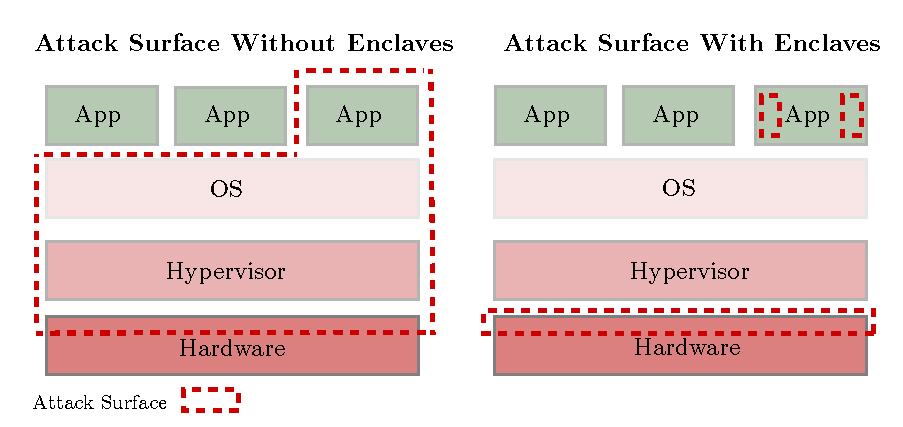
\includegraphics[width=\textwidth]{enclave}
	\caption[Attack surface with \acrshort{tee}]{
		Attack surface with \acrshort{tee}.
		Adapted from \url{sgx101.gitbook.io}.
	}%
	\label{figure:enclave}
\end{figure}


		While \acrshort{tee} is a concept defining an execution environment, specific solutions include a hardware security module (a plug-in device with a protected memory and a crypto-optimized processing unit), an \acrshort{fpga}, and a set of extensions to an existing processor architecture, such as an \acrshort{sgx} for Intel x86 or Secure Encrypted Virtualization \cite{amd-memory-encryption} for AMD\@.
		Of all these, Intel \acrshort{sgx} is the most widely used technology.

		\subsection{\texorpdfstring{\acrlong{sgx}}{Software Guard Extensions}}

			\acrfull{sgx} is a set of instructions for the Intel x86 architecture that allow a user or an \acrlong{os} to define a region of protected memory, called the \emph{enclave}, and interact with it.
			The enclave can only be accessed using the \acrshort{sgx} instructions (i.e, regular \texttt{mov} instruction would not work), and all pages of the enclave are symmetrically encrypted and physically protected.
			\acrshort{sgx} guarantees the integrity and security of the memory pages within the enclave.
			Although the size of enclave memory is very limited, \acrshort{sgx} can use regular \acrshort{ram} by transparently swapping the pages between the trusted and untrusted memory.
			The pages are then encrypted with integrity protection when placed in the \acrshort{ram} (\emph{sealing} in \acrshort{sgx} terms).

			An \acrshort{sgx}-enabled application declares its trusted and untrusted components upfront.
			Trusted part will live entirely in the enclave, while the untrusted part is a normal process that runs within the \acrshort{os}.
			The application has to be digitally signed for the enclave to accept it, and the enclave itself can authenticate to the user via an \emph{attestation} process.
			Conceptually, the simplest \acrshort{sgx} application in an outsourced database system can be seen as a trusted component that operates over sensitive material (e.g., keys, tokens, plaintext user data), a remote trusted client application that communicates with the enclave, and a layer of code that passes requests through (untrusted part of an \acrshort{sgx} application).
			Cipherbase \cite{cipherbase-daas} and StealthDB \cite{stealth-db} are good examples of such approach.

		\subsection{Issues with \acrshort{sgx}}

			\acrshort{sgx}, as the closest instantiation of \acrshort{tee} available, has been extensively targeted.
			The attacks include Foreshadow \cite{foreshadow}, Prime+Probe cache attack \cite{prime-probe-sgx-attack}, an attack from within the enclave \cite{enclave-sgx-attack}, Spectre line of attacks that can bypass \acrshort{sgx} \cite{spectre-sgx-attack}, replay attack \cite{replay-sgx-attack}, Plundervolt attack \cite{plundervolt-sgx-attack}, Load Value Injection attack \cite{lvi-sgx-attack} and SGAxe attack \cite{sgaxe-sgx-attack}.
			Due to its many security issues, \acrshort{sgx} has been officially discontinued.\footnote{As of $11^\text{th}$ Generation Intel Core processor.}

			Besides the attacks against the \acrshort{sgx}, the design itself has a number of restrictions.
			First of all, the enclave memory is capped at \SI{128}{\mega\byte}, part of which is occupied by the \acrshort{sgx} control structures, leaving the application about \SI{96}{\mega\byte}.
			\acrshort{sgx} allows the use of external memory pages through the sealing mechanism, but it imposes high overhead of re-encryption and crossing the enclave physical boundary.
			Second, the code execution inside the enclave is significantly slower.
			Third, by design, only the untrusted application component can interact with the \acrshort{os}, for example, make network or storage \acrshort{io} requests.
			Finally, from the security standpoint the enclave is vulnerable against the side-channel attacks, most of all, access pattern leakage.
			Such leakage implies that the normal database application cannot be placed directly in the enclave and be deemed secure, because access pattern has been effectively exploited up to a reconstruction attack \cite{generic-attacks-kellaris}.
			One then has to design the application specifically to conceal the access pattern.
			For example, ZeroTrace \cite{zerotrace} is a variant of PathORAM \cite{path-oram} that is internally oblivious and thus can work in \acrshort{sgx}.
			Oblix \cite{oblix} is another example of a structure that is, in \textcite{oblix} own terms, doubly-oblivious --- internally in how manages memory and registers, and externally in how it interacts with a storage.

	\section{Differentially private outsourced database systems}\label{section:range-persistent:dpodb}

	In this section we present our model, \emph{differentially private outsourced database system}, \acrshort{cdpodb}, its security definition, query types and efficiency measures.
	It is an extension of the outsourced database model in \cref{section:introduction:model:odb}.

	\subsection{Adversarial model}\label{section:range-persistent:dpodb:adversarial-models}

		We consider an honest-but-curious polynomial time adversary that attempts to breach differential privacy with respect to the input database \database{}.
		We observe later in \cref{section:range-persistent:dpodb:adversarial-models:adaptive} that it is impossible to completely hide the number of records returned on each query without essentially returning all the database records on each query.
		This, in turn, means that different query sequences may be distinguished, and, furthermore, that differential privacy may not be preserved if the query sequence depends on the content of the database records.
		We hence, only require the protection of differential privacy with respect to every fixed query sequence.
		Furthermore, we relax to computational differential privacy (following \cite{computational-dp}).

		In the following definition, the notation \view{\protocol{}}{\database, \fromNtoM{\query}{1}{m}} denotes the view of the server \server{} in the execution of protocol \protocol{} in answering queries \fromNtoM{\query}{1}{m} with the underlying database \database{}.

		\begin{definition}
			We say that an outsourced database system \protocol{} is $(\epsilon, \delta)$\hyp{}computationally differentially private (a.k.a.~\acrshort{cdpodb}) if for every polynomial time distinguishing adversary \adversary{}, for every neighboring databases $\database \sim \database^\prime$, and for every query sequence $\fromNtoM{\query}{1}{m} \in \querySet^m$ where $m = \mathsf{poly}(\lambda)$,

			\begin{multline*}
				\probability{\adversary \left( 1^\lambda, \view{\protocol{}}{\database, \fromNtoM{\query}{1}{m}} \right) = 1 } \leq \\
				\exp{(\epsilon)} \cdot \probability{\adversary \left( 1^\lambda, \view{\protocol{}}{\database^\prime, \fromNtoM{\query}{1}{m}} \right) = 1} + \delta +\negl \; ,
			\end{multline*}
			where the probability is over the randomness of the distinguishing adversary \adversary{} and the protocol \protocol{}.
		\end{definition}

	\begin{remark}[Informal]
		We note that security and differential privacy in this model imply protection against communication volume and access pattern leakages and thus prevent a range of attacks, such as \cite{leakage-abuse-attacks-cash-15,inference-attacks-naveed-15,generic-attacks-kellaris}. % chktex 2
	\end{remark}

	\subsubsection{On impossibility of adaptive queries}\label{section:range-persistent:dpodb:adversarial-models:adaptive}

		Non-adaptivity in our \acrshort{cdpodb} definition does not reflect a deficiency of our specific protocol but rather an inherent source of leakage when the queries may depend on the decrypted data.
		Consider an adaptive \acrshort{cdpodb} definition that does not fix the query sequence \fromNtoM{q}{1}{m} in advance but instead an arbitrary (efficient) user \user{} chooses them during the protocol execution with \server{}.
		As before, we ask that the \server{}'s view is \acrshort{dp} on neighboring databases for every such \user{}.
		We observe that this definition cannot possibly be satisfied by \emph{any} outsourced database system without unacceptable efficiency overhead.
		Note that non-adaptivity here does not imply that the client knows all the queries in advance, but rather can choose them at any time (e.g., depending on external circumstances) as long as they do not depend on true answers to prior queries.

		To see this, consider two neighboring databases $\database, \database^\prime$.
		Database \database{} has 1 record with $\mathsf{key} = 0$ and $\database^\prime$ has none.
		Furthermore, both have 50 records with $\mathsf{key} = 50$ and 100 records with $\mathsf{key} = 100$.
		User \user{} queries first for the records with $\mathsf{key} = 0$, and then if there is a record with $\mathsf{key} = 0$ it queries for the records with $\mathsf{key} = 50$, otherwise for the records with $\mathsf{key} = 100$.
		Clearly, an efficient outsourced database system cannot return nearly as many records when $\mathsf{key} = 50$ versus $\mathsf{key} = 100$ here.
		Hence, this allows distinguishing $\database, \database^\prime$ with probability almost 1.

		To give a concrete scenario, suppose neighboring medical databases differ in one record with a rare diagnosis ``Alzheimer's disease''.
		A medical professional queries the database for that diagnosis first (point query), and if there is a record, she queries the senior patients next (range query, \texttt{age $\ge$ 65}), otherwise she queries the general population (resulting in more records).
		We leave it open to meaningfully strengthen our definition while avoiding such impossibility results, and we defer the formal proof to future work.

	% chktex-file 1
% chktex-file 8
% chktex-file 21
% chktex-file 24
% chktex-file 26
% chktex-file 36
% chktex-file 37

\newlength{\setupLength}
\setlength{\setupLength}{17em}
\newlength{\queryLength}
\setlength{\queryLength}{16em}

\begin{algorithm*}[ht!]

	\begin{pcvstack}

		\procedure[linenumbering]{\protocolSetup{}}{
													\textbf{User \user}																\>																\> \textbf{Server \server}	\\
			%
			\label{algorithm:dp-oram:setup:line-2}	\pcinput{\database}																\>																\> \pcinput{\emptyset}		\\
			%
			\label{algorithm:dp-oram:setup:line-3}	\indexI \gets \algo{CreateIndex}{\database}										\>																\>							\\
			%
			\label{algorithm:dp-oram:setup:line-4}	\oramProgram = \left. (\oramWrite, \recordID_i, \record_i) \right|_{i = 1}^n	\>																\>							\\
			%
			\label{algorithm:dp-oram:setup:line-5}																					\> \sendmessageboth*[\setupLength]{\algo{ORAM}{\oramProgram}}	\>							\\
			%
			\label{algorithm:dp-oram:setup:line-6}	\serverDS \gets \algo{A}{\fromNtoM{\searchKey}{1}{\domainSize}}					\> \sendmessageright*[\setupLength]{\serverDS}					\>							\\
			%
			\label{algorithm:dp-oram:setup:line-7}	\pcouput{\indexI}																\>																\> \pcouput{\serverDS}
		}

		\vspace{0.5em}

		\procedure[linenumbering]{\protocolQuery{}}{
													\textbf{User \user}																				\>																											\> \textbf{Server \server}				\\
			%
			\label{algorithm:dp-oram:query:line-2}	\pcinput{\query, \indexI}																		\>																											\> \pcinput{\serverDS}					\\
			%
			\label{algorithm:dp-oram:query:line-3}	T \gets \algo{Lookup}{\indexI, \query}															\> \sendmessageright*[\queryLength]{\query}																	\> c \gets \algo{B}{\serverDS, \query}	\\
			%
			\label{algorithm:dp-oram:query:line-4}	\oramProgram_\mathsf{true} = \left. (\oramRead, \recordID_i, \bot) \right|_{i \in T}			\> \sendmessageleft*[\queryLength]{c}																		\>										\\
			%
			\label{algorithm:dp-oram:query:line-5}	\oramProgram_\mathsf{noise} = \left. (\oramRead, S \setminus T, \bot) \right|_{1}^{c - \abs{T}}	\>																											\>										\\
			%
			\label{algorithm:dp-oram:query:line-6}	R																								\> \sendmessageboth*[\queryLength]{\algo{ORAM}{\oramProgram_\mathsf{true} \| \oramProgram_\mathsf{noise}}}	\>										\\
			%
			\label{algorithm:dp-oram:query:line-7}	\pcouput{R}																						\>																											\>	\pcouput{\emptyset}
		}

	\end{pcvstack}

	\caption[\epsolute{} protocol]{
		\epsolute{} protocol.
		$\algo{ORAM}{\cdot}$ denotes an execution of \acrshort{oram} protocol (\cref{section:background:oram}), where \user{} plays the role of the client.
		\acrshort{oram} protocol client and server states are implicit.
		$S \setminus T$ represents a set of valid record IDs $S$ that are not in the true result set $T$.
	}%
	\label{algorithm:dp-oram}
\end{algorithm*}


	\subsection{Query types}

		In this work we are concerned with the following query types:
		\begin{description}[style=unboxed, leftmargin=0em]
			\item[Range queries]
				Here we assume a total ordering on \searchKeyDomain{}.
				A query \query{a}{b} is associated with an interval $\interval{a}{b}$ for $1 \leq a \leq b \leq \domainSize$ such that $\query{a}{b}(c) = 1$ iff $c \in \interval{a}{b}$ for all $c \in \searchKeyDomain$.
				The equivalent \acrshort{sql} query is:

				\smallskip
				\indent\texttt{SELECT * FROM table WHERE attribute BETWEEN a AND b;}
				\smallskip

			\item[Point queries]
				Here \searchKeyDomain{} is arbitrary and a query predicate \query{a} is associated with an element $a \in \searchKeyDomain$ such that $\query{a}(b) = 1$ iff $a = b$.
				In an ordered domain, point queries are degenerate range queries.
				The equivalent \acrshort{sql} query is:

				\smallskip
				\indent\texttt{SELECT * FROM table WHERE attribute = a;}

		\end{description}

	\subsection{Measuring Efficiency}

		We define two basic efficiency measures for a \acrshort{cdpodb}.
		\begin{description}[style=unboxed, leftmargin=0em]
			\item[Storage efficiency]
				is defined as the sum of the bit-lengths of the records in a database relative to the bit-length of a corresponding encrypted database.
				Specifically, we say that an outsourced database system has \emph{storage efficiency} of $(\efficiencyCoefficient, \efficiencyOffset)$ if the following holds.
				Fix any \databaseDef{} and let $n_1 = \sum_{i=1}^n \abs{r_i}$.
				Let $\server_\mathsf{state}$ be an output of \server{} on a run of \protocolSetup{} where \user{} has input \database{}, and let $n_2 = \abs{ \server_\mathsf{state} }$.
				Then $n_2 \leq \efficiencyCoefficient n_1 + \efficiencyOffset$.

			\item[Communication efficiency]
				is defined as the sum of the lengths of the records in bits whose search keys satisfy the query relative to the actual number of bits sent back as the result of a query.
				Specifically, we say that an outsourced database system has \emph{communication efficiency} of $(\efficiencyCoefficient, \efficiencyOffset)$ if the following holds.
				Fix any \query{} and \serverDS{} output by \protocolSetup{}, let \user{} and \server{} execute \protocolQuery{} where \user{} has inputs \query{}, and output $R$, and \server{} has input \serverDS{}.
				Let $m_1$ be the amount of data in bits transferred between \user{} and \server{} during the execution of \protocolQuery{}, and let $m_2 = \abs{ R }$.
				Then $m_2 \leq \efficiencyCoefficient m_1 + \efficiencyOffset$.
		\end{description}

		Note that $\efficiencyCoefficient \geq 1$ and $\efficiencyOffset \geq 0$ for both measures.
		We say that an outsourced database system is \emph{optimally storage efficient} (resp., \emph{optimally communication efficient}) if it has storage (resp., communication) efficiency of $(1, 0)$.

	\section{\texorpdfstring{\epsolute{}}{Epsolute}}\label{section:dp-oram}

	In this section we present a construction, \epsolute{}, that satisfies the security definition in \cref{section:dpodb}, detailing algorithms for both range and point query types.
	We also provide efficiency guarantees for approximate and pure \acrshort{dp} versions of \epsolute{}.

	\subsection{General construction}

		Let \querySet{} be a collection of queries.
		We are interested in building a differentially private outsourced database system for \querySet{}, called \epsolute{}.
		Our solution will use these building blocks.
		\begin{itemize}
			\item
				A $(\eta_1, \eta_2)$-\acrshort{oram} protocol \algo{ORAM}{\cdot}.
			\item
				An $(\epsilon, \delta, \alpha, \beta)$-differentially private sanitizer $(\algo{A}, \algo{B})$ for \querySet{} and negligible $\beta$, which satisfies the non-negative noise guarantee from \cref{remark:dp-sanitizer-guarantees}.
			\item
				A pair of algorithms \algo{CreateIndex} and \algo{Lookup}.
				\algo{CreateIndex} consumes \database{} and produces an index data structure \indexI{} that maps a search key \searchKey{} to a list of record IDs \recordID{} corresponding to the given search key.
				\algo{Lookup} consumes \indexI{} and \query{} and returns a list $T = \fromNtoM{\recordID}{1}{{\abs{T}}}$ of record IDs matching the supplied query.
		\end{itemize}

		Our protocol $\protocol = (\protocolSetup, \protocolQuery)$ of \epsolute{} works as shown in \cref{algorithm:dp-oram}.
		Hereafter, we reference lines in \cref{algorithm:dp-oram}.
		See \cref{figure:dp-oram} for a schematic description of the protocol.

		\paragraph*{Setup protocol \; \texorpdfstring{\protocolSetup{}}{}}

			Let \user{}'s input be a database \databaseDef{} (\cref{algorithm:dp-oram:setup:line-2}).
			\user{} creates an index \indexI{} mapping search keys to record IDs corresponding to these keys (\cref{algorithm:dp-oram:setup:line-3}).
			\user{} sends over the records to \server{} by executing the \acrshort{oram} protocol on the specified sequence (\crefrange{algorithm:dp-oram:setup:line-4}{algorithm:dp-oram:setup:line-5}).
			\user{} generates a \acrshort{dp} structure \serverDS{} over the search keys using sanitizer \algo{A}, and sends \serverDS{} over to \server{} (\cref{algorithm:dp-oram:setup:line-6}).
			The output of \user{} is \indexI{} and of \server{} is \serverDS{}; final \acrshort{oram} states of \server{} and \user{} are implicit, including encryption key \queryKey{} (\cref{algorithm:dp-oram:setup:line-7}).

		\paragraph*{Query protocol \; \texorpdfstring{\protocolQuery{}}{}}

			\user{} starts with a query \query{} and index \indexI{}, \server{} starts with a \acrshort{dp} structure \serverDS{}.
			One can think of these inputs as outputs of \protocolSetup{} (\cref{algorithm:dp-oram:query:line-2}).
			\user{} immediately sends the query to \server{}, which uses the sanitizer \algo{B} to compute the total number of requests $c$, while \user{} uses index \indexI{} to derive the true indices of the records the query \query{} targets (\cref{algorithm:dp-oram:query:line-3}).
			\user{} receives $c$ from \server{} and prepares two \acrshort{oram} sequences: $\oramProgram_\mathsf{true}$ for real records retrieval, and $\oramProgram_\mathsf{noise}$ to pad the number of requests to $c$ to perturb the communication volume.
			$\oramProgram_\mathsf{noise}$ includes valid non-repeating record IDs that are not part of the true result set $T$ (\crefrange{algorithm:dp-oram:query:line-4}{algorithm:dp-oram:query:line-5}).
			\user{} fetches the records, both real and fake, from \server{} using the \acrshort{oram} protocol (\cref{algorithm:dp-oram:query:line-6}).
			The output of \user{} is the filtered set of records requested by the query $\query{}$; final \acrshort{oram} states of \server{} and \user{} are implicit (\cref{algorithm:dp-oram:query:line-7}).

		The protocols for point and range queries only differ in sanitizer implementations, see \cref{section:dp-oram:point,section:dp-oram:range}.
		Note above that in any execution of \protocolQuery{} we have $c \geq \query(\database)$ with overwhelming probability $1 - \beta$ (by using sanitizers satisfying \cref{remark:dp-sanitizer-guarantees}), and thus the protocol is well-defined and its accuracy is $1 - \beta$.
		Also note that the \acrshort{dp} parameter $\delta$ is lower-bounded by $\beta$ because sampling negative noise, however improbable, violates privacy, and therefore the final construction is $(\epsilon, \beta)$-\acrshort{dp}.

		\begin{figure}[!ht]
	\centering
	\includegraphics[width=\linewidth]{dp-oram}
	\caption{\epsolute{} construction}%
	\label{figure:dp-oram}
\end{figure}


	\subsection{Security}

		\begin{theorem}
			\epsolute{} is $(\beta \cdot m)$-wrong and $(\epsilon, \delta)$-\acrshort{cdpodb} where the negligible term is $\negl = 2 \cdot \eta_2$.
		\end{theorem}

		\begin{proof}
			We consider a sequence of views
			\[
				\view{1} \to \view{2} \to \view{3} \to \view{4} \; .
			\]
			\view{1} is \view{\protocol}{\database, \fromNtoM{\query}{1}{m}}.
			\view{2} is produced only from $\serverDS \gets \algo{A}{\fromNtoM{\searchKey}{1}{\domainSize}}$.
			Namely, compute $c_i \gets \algo{A}{\serverDS, \query_i}$ for all $i$ and run \acrshort{oram} simulator on $\sum_i c_i$.
			By \acrshort{oram} security,
			\[
				\probability{\adversary(\view{1})} - \probability{\adversary(\view{2})} \leq \eta_2 \; .
			\]
			\view{3} is produced similarly but $\serverDS \gets \algo{A}{\fromNtoM{\searchKey^\prime}{1}{\domainSize}}$ instead.
			Note that the $c_i$ are simply post-processing on \serverDS{} via \algo{B} so
			\[
				\probability{\adversary(\view{2})} = \exp(\epsilon) \cdot \probability{\adversary(\view{3})} + \delta \; .
			\]
			$\view{4} = \view{\protocol}{\database^\prime, \fromNtoM{\query}{1}{m}}$.
			It follows by \acrshort{oram} security
			\[
				\probability{\adversary(\view{3})} - \probability{\adversary(\view{4})} \leq \eta_2 \; .
			\]
			Putting this all together completes the proof.
		\end{proof}

	\subsection{Efficiency}

		For an \acrshort{oram} with communication efficiency $(a_1, a_2)$ and an $(\alpha, \beta)$-differentially private sanitizer, the \epsolute{} communication efficiency is $(a_1, a_2 \cdot \alpha)$.
		The efficiency metrics demonstrate how the total storage or communication volume (the number of stored or transferred bits) changes additively and multiplicatively as the functions of data size \dataSize{} and domain \domainSize{}.
		We therefore have the following corollaries for the efficiency of the system in the cases of approximate and pure differential privacy.
		\begin{corollary}\label{corollary:comm-efficiency-approximate-dp}
			\epsolute{} is an outsourced database system with storage efficiency \efficiency{1}{0}.
			Depending on the query type, assume it offers the following communication efficiency.
			\begin{description}
				\item[Range queries] $\efficiency{\log \dataSize}{2^{\log^* \domainSize} \log \dataSize}$
				\item[Point queries] $\efficiency{\log \dataSize}{\log \dataSize}$
			\end{description}
			Then, there is a negligible $\delta$ such that \epsolute{} satisfies $(\epsilon, \delta)$\hyp{}differential privacy for some $\epsilon$.\footnote{
				Note that the existence of $\epsilon$ in this setting implies that the probability of an adversary breaking the \acrshort{dp} guarantees is bounded by it.
			}
		\end{corollary}

		\begin{proof}
			By using \acrshort{oram}, we store only the original data once and hence, we get optimal storage efficiency.

			The communication efficiency depends on the upper bound of the error for each sanitizer when $\delta > 0$, as described in \cref{section:building-blocks:dp} and \cref{remark:dp-sanitizer-guarantees}.
			The most efficient \acrshort{oram} protocol to date has $\bigO{\log \dataSize}$ communication overhead (see \cref{section:building-blocks:oram}).
		\end{proof}

		\begin{corollary}\label{corollary:comm-efficiency-pure-dp}
			\epsolute{} is an outsourced database system with storage efficiency \efficiency{1}{0}.
			Depending on the query type, assume it offers the following communication efficiency.
			\begin{description}
				\item[Range queries] $\efficiency{\log \dataSize}{\log \domainSize \log \dataSize}$
				\item[Point queries] $\efficiency{\log \dataSize}{\log \domainSize \log \dataSize}$
			\end{description}
			Then, \epsolute{} satisfies $\epsilon$-differential privacy for some $\epsilon$.
		\end{corollary}

		\begin{proof}
			Similarly, we derive the proof by considering the use of \acrshort{oram} and the upper bound of the error for each sanitizer when $\delta = 0$ in \cref{section:building-blocks:dp}.
		\end{proof}

	\subsection{Extending to multiple attributes}\label{section:dp-oram:multiple-attributes}

		We will now describe how \epsolute{} supports multiple indexed attributes and what the privacy and performance implications are.
		The na\"{\i}ve way is to simply duplicate the entire stack of states of \user{} and \server{}, and during the query use the states whose attribute the query targets.
		However, \epsolute{} design allows to keep the most expensive part of the state --- the \acrshort{oram} state --- shared for all attributes and both types of queries.
		Specifically, the index \indexI{} and \acrshort{dp} structure \serverDS{} are generated per attribute and query type, while \user{} and \server{} \acrshort{oram} states are generated once.
		This design is practical since \serverDS{} is tiny and index \indexI{} is relatively small compared to \acrshort{oram} states, see \cref{section:experiments}.

		We note that in case the indices grow large in number, it is practical to outsource them to the adversarial server using \acrshort{oram} and download only the ones needed for each query.
		In terms of privacy, the solution is equivalent to operating different \epsolute{} instances because \acrshort{oram} hides the values of records and access patterns entirely.
		Due to \cref{theorem:composition} for non-disjoint datasets, the total privacy budget of the multi-attribute system will be the sum of individual budgets for each attribute / index.

		Next, we choose two \acrshort{dp} sanitizers for our system, for point and for range queries, and calculate the $\alpha$ values to make them output positive values with high probability, consistent with \cref{remark:dp-sanitizer-guarantees}.

	\subsection{\texorpdfstring{\epsolute{}}{Epsolute} for point queries}\label{section:dp-oram:point}

		For point queries, we use the \acrshort{lpa} method as the sanitizer to ensure pure differential privacy.
		Specifically, for every histogram bin, we draw noise from the Laplace distribution with mean $\alpha_p$ and scale $\lambda = \nicefrac{1}{\epsilon}$.
		To satisfy \cref{remark:dp-sanitizer-guarantees}, we have to set $\alpha_p$ such that if values are drawn from $\algo{Laplace}{ \alpha_p, \nicefrac{1}{\epsilon} }$ at least as many times as the number of bins \domainSize{}, they are all positive with high probability $1 - \beta$, for negligible $\beta$.

		We can compute the exact minimum required value of $\alpha_p$ in order to ensure drawing positive values with high probability by using the \acrshort{cdf} of the Laplace distribution.
		Specifically, $\alpha_p$ should be equal to the minimum value that satisfies the following inequality.

		\[
			\left( 1 - \frac{1}{2} e^{- \alpha_p \cdot \epsilon} \right)^\domainSize \leq 1 - \beta
		\]
		which is equivalent to
		\[
			\alpha_p = \ceil{ -\frac{ \ln \left( 2 - 2 \sqrt[\domainSize]{1 - \beta} \right) }{ \epsilon } }
		\]

	% chktex-file 1
% chktex-file 8
% chktex-file 21
% chktex-file 24
% chktex-file 26
% chktex-file 36
% chktex-file 37

\setlength{\setupLength}{16em}
\setlength{\queryLength}{15em}

\newcommand{\SetupGamma}{
	\procedure[linenumbering]{\protocolSetup{} of \protocolGamma{}}{
																\textbf{User \user}																							\>																\> \textbf{Server \server}	\\
		%
		\label{algorithm:dp-oram-parallel:gamma:setup:line-2}	\pcinput{\database{}}																						\>																\> \pcinput{\emptyset}		\\
		%
		\label{algorithm:dp-oram-parallel:gamma:setup:line-3}	\indexI \gets \algo{CreateIndex}{\database, \oramsNumber}													\>																\>							\pclb
		%
		\pcintertext[dotted]{$\pcfor j \in \set{1, \ldots, \oramsNumber} \pcdo$ \; \text{(in parallel)}}
		%
		\label{algorithm:dp-oram-parallel:gamma:setup:line-4}	\left\langle \overline{\record}, \overline{\recordID} \right\rangle\ \text{s.t.}\ \algo{H}{\recordID} = j	\>																\>							\\
		%
		\label{algorithm:dp-oram-parallel:gamma:setup:line-5}	\oramProgram = \left\langle (\oramWrite, \overline{\recordID}, \overline{\record}) \right\rangle			\> \sendmessageboth*[\setupLength]{\algo{ORAM}_j(\oramProgram)}	\>							\pclb
		%
		\pcintertext[dotted]{$\pcendfor$}
		%
		\label{algorithm:dp-oram-parallel:gamma:setup:line-6}	\serverDS \gets \algo{A}{\fromNtoM{\searchKey}{1}{\domainSize}}												\> \sendmessageright*[\setupLength]{\serverDS}					\>							\\
		%
		\label{algorithm:dp-oram-parallel:gamma:setup:line-7}	\pcouput{\indexI}																							\>																\> \pcouput{ \serverDS }
	}
}

\newcommand{\QueryGamma}{
	\procedure[linenumbering]{\protocolQuery{} of \protocolGamma{}}{
																\textbf{User \user}																					\>																												\> \textbf{Server \server}									\\
		%
		\label{algorithm:dp-oram-parallel:gamma:query:line-2}	\pcinput{\query, \indexI}																			\>																												\> \pcinput{ \serverDS }									\\
		%
		\label{algorithm:dp-oram-parallel:gamma:query:line-3}	\fromNtoM{T}{1}{\oramsNumber} \gets \algo{Lookup}{I, \query}										\> \sendmessageright*[\queryLength]{\query}																		\> k \gets \algo{B}{\serverDS, \query}						\\
		%
		\label{algorithm:dp-oram-parallel:gamma:query:line-4}																										\> \sendmessageleft*[\queryLength]{c}																			\> c \gets (1 + \gamma) \frac{\tilde{k}_0}{\oramsNumber}	\pclb
		%
		\pcintertext[dotted]{$\pcfor j \in \set{1, \ldots, \oramsNumber} \pcdo$ \; \text{(in parallel)}}
		%
		\label{algorithm:dp-oram-parallel:gamma:query:line-5}	\oramProgram_\mathsf{true} = \left. (\oramRead, \recordID_i, \bot) \right|_{i \in T_j}				\>																												\>															\\
		%
		\label{algorithm:dp-oram-parallel:gamma:query:line-6}	\oramProgram_\mathsf{noise} = \left. (\oramRead, S \setminus T_j, \bot) \right|_{1}^{c - \abs{T_j}}	\> \sendmessageboth*[\queryLength]{\algo{ORAM}_j(\oramProgram_\mathsf{true} \| \oramProgram_\mathsf{noise})}	\> R_j														\pclb
		%
		\pcintertext[dotted]{$\pcendfor$}
		%
		\label{algorithm:dp-oram-parallel:gamma:query:line-7}	\pcouput{ \left. R_j \right|_{j = 1}^\oramsNumber }													\>																												\>	\pcouput{\emptyset}
	}
}

\begin{algorithm*}[ht!]

	\begin{pcvstack}

		\begin{pcvstack}

			\SetupGamma{}

			\vspace{0.5em}

			\QueryGamma{}

		\end{pcvstack}

	\end{pcvstack}

	\caption[Parallel \epsolute{} for \protocolGamma{}]{
		Parallel \epsolute{} for \protocolGamma{}, extends \cref{algorithm:dp-oram}.
		\algo{H} is a random hash function $\algo{H} : \bin^* \to \set{1, \ldots, \oramsNumber}$.
		$\gamma$ and $\tilde{k}_0$ are computed as in \cref{section:range-persistent:prallel-dp-oram:gamma}.
	}%
	\label{algorithm:dp-oram-parallel}
\end{algorithm*}


	\subsection{\texorpdfstring{\epsolute{}}{Epsolute} for range queries}\label{section:dp-oram:range}

		For range queries, we implement the aggregate tree method as the sanitizer.
		Specifically, we build a complete \fanout{}-ary tree on the domain, for a given \fanout{}.
		A leaf node holds the number of records falling into each bin plus some noise.
		A parent node holds sum of the leaf values in the range covered by this node, plus noise.
		Every time a query is issued, we find the minimum number of nodes that cover the range, and determine the required number of returned records by summing these node values.
		Then, we ask the server to retrieve the records in the range, plus to retrieve multiple random records so that the total number of retrieved records matches the required number of returned records.

		The noise per node is drawn from the Laplace distribution with mean $\alpha_h$ and scale $\lambda = \frac{\log_{\fanout} \domainSize}{\epsilon}$.
		Consistent with \cref{remark:dp-sanitizer-guarantees}, we determine the mean value $\alpha_h$ in order to avoid drawing negative values with high probability.
		We have to set $\alpha_h$ such that if values are drawn from $\algo{Laplace}{ \alpha_h, \frac{\log_{\fanout} \domainSize}{\epsilon} }$ at least as many times as the number of nodes in the tree, they are all positive with high probability $1 - \beta$, for negligible $\beta$.

		Again, we can compute the exact minimum required value of $\alpha_h$ in order to ensure drawing positive values with high probability by using the \acrshort{cdf} of the Laplace distribution.
		Specifically, $\alpha_h$ should be equal to the minimum value that satisfies the following inequality.
		\[
			\left( 1 - \frac{1}{2} e^{- \frac{\alpha_h \cdot \epsilon}{\log_{\fanout} \domainSize}} \right)^\mathsf{nodes} \leq 1 - \beta
		\]
		which is equivalent to
		\begin{equation}\label{equation:min-mu-for-range}
			\alpha_h = \ceil{ -\frac{ \ln{ (2 - 2 \sqrt[\mathsf{nodes}]{ 1 - \beta } ) } \cdot \log_{\fanout} \domainSize }{\epsilon} }
		\end{equation}
		where $\mathsf{nodes} = \frac{ \fanout^{ \ceil{ \log_{\fanout} (\fanout - 1) + \log_{\fanout} \domainSize - 1 }} - 1}{ \fanout - 1 } + \domainSize$ is the total number of tree nodes.

	\section{An efficient Parallel \texorpdfstring{\epsolute{}}{Epsolute}}\label{section:range-persistent:prallel-dp-oram}

	While the previously described scheme is a secure and correct \acrshort{cdpodb}, a single-threaded implementation may be prohibitively slow in practice.
	To bring the performance closer to real-world requirements, we need to be able to scale the algorithm horizontally.
	In this section, we describe an upgrade of \epsolute{} --- a scalable parallel solution.

	We suggest two variants of parallel \epsolute{} protocol.
	Both of them work by operating \oramsNumber{} \acrshortpl{oram} and randomly assigning to each of them $\nicefrac{n}{\oramsNumber}$ database records.
	For each query, we utilize the index \indexI{} to find the required records from the corresponding \acrshortpl{oram}.
	For each \acrshort{oram}, we execute a separate thread to retrieve the records.
	The threads work in parallel and there is no need for locking, since each \acrshort{oram} works independently from the rest.
	We present two methods that differ in the way they build and store \acrshort{dp} structure \serverDS{}, and hence the number of \acrshort{oram} requests they make.

	\subsection{\texorpdfstring{No-$\gamma$-method}{No-gamma-method}: \acrshort{dp} structure per \acrshort{oram}}

		In \protocolNoGamma{}, for each \acrshort{oram} / subset of the dataset, we build a \acrshort{dp} index the same way as described in \cref{section:range-persistent:dp-oram}.
		We note that \cref{theorem:composition} for disjoint datasets applies to this construction: the privacy budget $\epsilon$ for the construction is the largest (least private) among the $\epsilon$'s of the \acrshort{dp} indices for each \acrshort{oram} / subset of the dataset.

		The communication efficiency changes because
		\begin{enumerate*}[label={(\roman*)}]
			\item
				we essentially add \oramsNumber{} record subsets in order to answer a query, each having at most $\alpha$ extra random records, and
			\item
				each \acrshort{oram} holds fewer records than before, resulting in a tree of height $\log \frac{\dataSize}{\oramsNumber}$.
		\end{enumerate*}

		However, we cannot expect that the records required for each query are equally distributed among the different \acrshortpl{oram} in order to reduce the multiplicative communication cost from $\log \dataSize$ to $\frac{\log \dataSize}{\oramsNumber}$.
		Instead, we need to bound the worst case scenario which is represented by the maximum number of records from any \acrshort{oram} that is required to answer a query.
		This can be computed as follows.

		Let $X_j$ be $1$ if a record for answering query \query{} is in a specific $\algo{ORAM}_j$, and $0$ otherwise.
		Due to the random assignment of records to \acrshortpl{oram}, $\probability{X_j = 1} = \nicefrac{1}{\oramsNumber}$.
		Assume that we need $k_0$ records in order to answer query \query{}.
		The maximum number of records from $\algo{ORAM}_j$ in order to answer \query{} is bounded as follows.

		\begin{equation}\label{equation:gamma}
			\probability{ \sum_{i=1}^{k_0} X_i > ( 1 + \gamma ) \frac{k_0}{\oramsNumber} } \leq \exp{ \left( - \frac{ k_0 \gamma^2 }{ 3 \oramsNumber } \right) }
		\end{equation}

		Finally, we need to determine the value of $\gamma$ such that $\exp{ \left( - \frac{ k_0 \gamma^2 }{ 3 \oramsNumber } \right) }$ is smaller than the value $\beta$.
		Thus, $\gamma = \sqrt{ \frac{-3 \oramsNumber \log \beta}{ k_0 } }$.
		The communication efficiency for each query type is described in the following corollary.

		\begin{corollary}\label{corollary:no-gamma}
			Let \protocolNoGamma{} be an outsourced database system with storage efficiency \efficiency{1}{0}.
			Depending on the query type, \protocolNoGamma{} offers the following communication efficiency.
			\begin{description}
				\item[Range queries] $\efficiency{\left( 1 + \sqrt{ \frac{- 3 \oramsNumber \log \beta}{k_0} } \right) \log \frac{\dataSize}{\oramsNumber} }{ \frac{ \log^{1.5} \domainSize}{ \epsilon } \oramsNumber \log \dataSize }$
				\item[Point queries] $\efficiency{\left( 1 + \sqrt{ \frac{- 3 \oramsNumber \log \beta}{k_0} } \right) \log \frac{\dataSize}{\oramsNumber} }{ \frac{ \log \domainSize}{ \epsilon } \oramsNumber \log \dataSize }$
			\end{description}

			Then, \protocolNoGamma{} satisfies $\epsilon$-differential privacy for some $\epsilon$.
		\end{corollary}

		In our experiments, we set \oramsNumber{} as a constant depending on the infrastructure.
		However, if \oramsNumber{} is set as $\bigO{\log n}$, the total communication overhead of the construction will still exceed the lower-bound presented in \cite{multi-server-orams}.

	\subsection{\texorpdfstring{$\gamma$-method}{Gamma-method}: shared \acrshort{dp} structure}\label{section:range-persistent:prallel-dp-oram:gamma}

		In \protocolGamma{}, we maintain a single shared \acrshort{dp} structure \serverDS{}.
		When a query is issued, we must ensure that the number of records retrieved from every \acrshort{oram} is the same.
		As such, depending on the required noisy number of records $\tilde{k}_0$, we need to retrieve at most $( 1 + \gamma ) \frac{ \tilde{k}_0 }{\oramsNumber}$ records from each \acrshort{oram}, see \cref{equation:gamma}, for $\gamma = \sqrt{ \frac{-3 \oramsNumber \log \beta}{ \tilde{k}_0 } }$.
		Setting $\tilde{k}_0 = k_0 + \frac{\log^{1.5} \domainSize}{\epsilon}$ for range queries and $\tilde{k}_0 = k_0 + \frac{\log \domainSize}{\epsilon}$ for point queries, the communication efficiency is as follows.

		\begin{corollary}\label{corollary:gamma}
			Let \protocolGamma{} be an outsourced database system with storage efficiency \efficiency{1}{0}.
			Depending on the query type, \protocolGamma{} offers the following communication efficiency.
			\begin{description}
				\item[Range queries] $\efficiency{ \left( 1 + \sqrt{ \frac{-3 \oramsNumber \log \beta}{k_0 + \frac{ \log^{1.5} \domainSize }{ \epsilon }} }\right) \log \frac{\dataSize}{\oramsNumber} \left( 1 + \frac{\log^{1.5} \domainSize}{\epsilon} \right) }{0}$
				\item[Point queries] $\efficiency{ \left( 1 + \sqrt{ \frac{-3 \oramsNumber \log \beta}{k_0 + \frac{ \log \domainSize }{ \epsilon }} }\right) \log \frac{\dataSize}{\oramsNumber} \left( 1 + \frac{\log \domainSize}{\epsilon} \right) }{0}$
			\end{description}
			Then, \protocolGamma{} satisfies $\epsilon$-differential privacy for some $\epsilon$.
		\end{corollary}

		\protocolGamma{} is depicted in \cref{algorithm:dp-oram-parallel}.
		There are a few extensions to the subroutines and notation from \cref{algorithm:dp-oram}.
		\algo{CreateIndex} and \algo{Lookup} now build and query the index which maps a search key to a pair --- the record ID and the \acrshort{oram} ID (1 to \oramsNumber{}) which stores the record.
		\Crefrange{algorithm:dp-oram-parallel:gamma:setup:line-4}{algorithm:dp-oram-parallel:gamma:setup:line-6} of \cref{algorithm:dp-oram-parallel} \protocolSetup{} repeat for each \acrshort{oram} and operate on the records partitioned for the given \acrshort{oram} using hash function \algo{H} on the record ID\@.
		A shared \acrshort{dp} structure is created with the sanitizer \algo{A} (\cref{algorithm:dp-oram-parallel:gamma:setup:line-7}).
		In \cref{algorithm:dp-oram-parallel} \protocolQuery{}, the total number of \acrshort{oram} requests is computed once (\cref{algorithm:dp-oram-parallel:gamma:query:line-4}).
		\Crefrange{algorithm:dp-oram-parallel:gamma:query:line-5}{algorithm:dp-oram-parallel:gamma:query:line-7} repeat for each \acrshort{oram} and operate on the subset of records stored in the given \acrshort{oram}.
		Note that \user{} and \server{} implicitly maintain \oramsNumber{} \acrshort{oram} states, and the algorithm uses the $(\algo{A}, \algo{B})$ sanitizer defined in \cref{section:range-persistent:dp-oram}.

		Note that we guarantee privacy and access pattern protection on a record level.
		Each \acrshort{oram} gets accessed at least once (much more than once for a typical query) thus the existence of a particular result record in a particular \acrshort{oram} is hidden.

	\subsection{Practical improvements}\label{section:range-persistent:dp-improvements}

		Here we describe the optimizations aimed at bringing the construction's performance to the real-world demands.

		\subsubsection{\texorpdfstring{\acrshort{oram}}{ORAM} request batching}\label{section:range-persistent:dp-improvements:oram-batching}

			We have noticed that although the entire set of \acrshort{oram} requests for each query is known in advance, the requests are still executed sequentially.
			To address this inefficiency, we have designed a way to combine the requests in a batch and reduce the number of network requests to the bare minimum.
			We have implemented this method over PathORAM, which we use for the $(\eta_1, \eta_2)$-\acrshort{oram} protocol, but the idea applies to most tree-based \acrshortpl{oram} (similar to \cite{parallel-oram-improved}).

			Our optimization utilizes the fact that all PathORAM leaf IDs are known in advance and paths in a tree-based storage share the buckets close to the root.
			The core idea is to read all paths first, processes the requests and and then write all paths back.
			This way the client makes a single \texttt{read} request, which is executed much faster than many small requests.
			Requests are then processed in main memory, including re-encryptions.
			Finally, the client executes the \texttt{write} requests using remapped leaves as a single operation, saving again compared to sequential execution.

			This optimization provides up to \textbf{8 times} performance boost in our experiments.
			We note that the gains in speed and \acrshort{io} overhead are achieved at the expense of main memory, which is not an issue given that the memory is released after a batch, and our experiments confirm that.
			The security guarantees of PathORAM are maintained with this optimization, since the security proof in \cite[Section 3.6]{path-oram} still holds. % chktex 2
			Randomized encryption, statistically independent remapping of leaves, and stash processing do not change.

		\subsubsection{Lightweight \texorpdfstring{\acrshort{oram}}{ORAM} servers}\label{section:range-persistent:dp-improvements:three-tier}

			We have found in our experiments that na\"{\i}ve increase of the number of \acrshort{cpu} cores and gigabytes of memory does not translate into linear performance improvement after some threshold.
			Investigating the observation we have found that the \epsolute{} protocol, executing parallel \acrshort{oram} protocols, is highly intensive with respect to main memory access, cryptographic operations and network usage.
			The bottleneck is the hardware --- we have confirmed that on a single machine the memory and network are saturated quickly preventing the linear scaling.

			\begin{figure}[ht!]
	\centering
	\includegraphics[width=\linewidth]{three-layers}
	\caption[Lightweight \acrshort{oram} machines diagram]{
		Lightweight \acrshort{oram} machines diagram.
		A \emph{user} sends a query to \user{} modeled as the \emph{client} machine, which uses local \emph{data index} and \emph{\acrshort{dp} structures} to prepare a set of \acrshort{oram} requests, which are sent to respective \emph{\acrshort{oram} machines}.
		These machines execute the \acrshort{oram} protocol against the \emph{untrusted storage} of \server{}.
	}%
	\label{figure:three-tier}
\end{figure}


			To address the problem, we split the user party \user{} into multiple lightweight machines that are connected locally to each other and reside in a single trust domain (e.g., same data center).
			Specifically, we maintain a \emph{client machine} that receives user requests and prepares \acrshort{oram} \texttt{read} requests, and up to \oramsNumber{} lightweight \emph{\acrshort{oram} machines}, whose only job is to run the \acrshort{oram} protocols in parallel.
			See \cref{figure:three-tier} for the schematic representation of the architecture.
			We emphasize that \user{} is still a single party, therefore, the security and correctness guarantees remain valid.

			The benefit of this approach is that each of the lightweight machines has its own hardware stack.
			Communication overhead among \user{} machines is negligible compared to the one between \user{} and \server{}.
			The approach is also flexible: it is possible to use up to \oramsNumber{} \acrshort{oram} machines and the machines do not have to be identical.
			Our experiments show that when the same number of \acrshort{cpu} cores and amount of memory are consumed the efficiency gain is up to \textbf{5 times}.

	\section{Experimental Evaluation}\label{section:range-persistent:experiments}

	We have implemented our solution as a modular client-server application in C++.
	We open-sourced all components of the software set: PathORAM \cite{github-path-oram} and B+ tree \cite{github-b-plus-tree} implementations and the main query executor \cite{github-epsolute}.
	We provide PathORAM and B+ tree components as C++ libraries to be used in other projects; the code is documented, benchmarked and tested (228 tests covering \SI{100}{\percent} of the code).
	We have also published our datasets and query sets \cite{our-datasets}.

	For cryptographic primitives, we used OpenSSL library (version 1.1.1i).
	For symmetric encryption in \acrshort{oram} we have used \acrshort{aes} in CBC mode \cite{nist-aes,nist-modes} with a 256-bits key (i.e., $\eta_2 = 2^{-256}$), for the hash algorithm \algo{H} used to partition records among \acrshortpl{oram} we have used \acrshort{sha}-256 algorithm \cite{nist-hash}.
	Aggregate tree fanout \fanout{} is 16, proven to be optimal in \cite{hierarchical-methods-for-dp}.

	We designed our experiments to answer the following questions:
	\newlength{\questionLength}
	\settowidth{\questionLength}{Question-5}
	\begin{description}[
		font=\bfseries,
		leftmargin=\dimexpr\questionLength+1.0em\relax,
		labelindent=0pt,
		labelwidth=\questionLength%
	]
		\item[Question-1\label{item:question-practicality}] How practical is our system compared to the most efficient and most private real-world solutions?
		\item[Question-2\label{item:question-storage}] How practical is the storage overhead?
		\item[Question-3\label{item:question-parameters}] How different inputs and parameters of the system affect its performance?
		\item[Question-4\label{item:question-scalability}] How well does the system scale?
		\item[Question-5\label{item:question-optimizations}] What improvements do our optimizations provide?
		\item[Question-6\label{item:question-attributes}] What is the impact of supporting multiple attributes?
	\end{description}

	To address \ref{item:question-practicality} we have run the default setting using conventional \acrshort{rdbms} (MySQL and PostgreSQL), Linear Scan approach and Shrinkwrap \cite{shrinkwrap}. % chktex 2
	To target \ref{item:question-storage}, we measured the exact storage used by the client and the server for different data, record and domain sizes. % chktex 2
	To answer \ref{item:question-parameters}, we ran a default setting and then varied all parameters and inputs, one at a time. % chktex 2
	For \ref{item:question-scalability} we gradually added \acrshortpl{cpu}, \acrshort{oram} servers and \acrshort{kvs} instances and observed the rate of improvement in performance. % chktex 2
	For \ref{item:question-optimizations} we have run the default setting with our optimizations toggled. % chktex 2
	Lastly, for \ref{item:question-attributes} we have used two datasets to construct two indices and then queried each of the attributes. % chktex 2

	\subsection{Data sets}\label{section:range-persistent:experiments:data-sets}

		We used two real and one synthetic datasets --- California public pay pension database 2019 \cite{ca-employees-dataset} (referred to as ``CA employees''), Public Use Microdata Sample from US Census 2018 \cite{pums-dataset} (referred to as ``PUMS'') and synthetic uniform dataset.
		We have used salary / wages columns of the real datasets, and the numbers in the uniform set also represent salaries.
		The \texttt{NULL} and empty values were dropped.

		We created three versions of each dataset --- $10^5$, $10^6$ and $10^7$ records each.
		For uniform dataset, we simply generated the target number of entries.
		For PUMS dataset, we picked the states whose number of records most closely matches the target sizes (Louisiana for $10^5$, California for $10^6$ and the entire US for $10^7$).
		Uniform dataset was also generated for different domain sizes --- number of distinct values for the record.
		For CA employees dataset, the set contains \num{260 277} records, so we contracted it and expanded in the following way.
		For contraction we uniformly randomly sampled $10^5$ records.
		For expansion, we computed the histogram of the original dataset and sampled values uniformly within the bins.

		Each of the datasets has a number of corresponding query sets.
		Each query set has a selectivity or range size, and is sampled either uniformly or following the dataset distribution (using its \acrshort{cdf}).

	\subsection{Default setting}\label{section:range-persistent:experiments:default-setting}

		The default setting uses the \protocolGamma{} from \cref{section:range-persistent:prallel-dp-oram} and lightweight \acrshort{oram} machines from \cref{section:range-persistent:dp-improvements:three-tier,figure:three-tier}.
		We choose the \protocolGamma{} because it outperforms \protocolNoGamma{} in all experiments (see \textbf{\ref{item:question-scalability}} in \cref{section:range-persistent:experiments:results}).
		In the setting, there are 64 Redis services (8 services per one Redis server \acrshort{vm}), 8 \acrshort{oram} machines communicating with 8 Redis services each, and the client, which communicates with these 8 \acrshort{oram} machines.
		We have empirically found this configuration optimal for the compute nodes and network that we used in the experiments.
		\acrshort{oram} and Redis servers run on GCP \texttt{n1-standard-16} \acrshortpl{vm} (Ubuntu 18.04), in regions \texttt{us-east4} and \texttt{us-east1} respectively.
		Client machine runs \texttt{n1-highmem-16} \acrshort{vm} in the same region as \acrshort{oram} machines.
		The ping time between the regions (i.e.\ between trusted and untrusted zones) is \SI{12}{\milli\second} and the effective bandwidth is \SI{150}{\mega\byte\per\second}.
		Ping within a region is negligible.

		Default \acrshort{dp} parameters are $\epsilon = \ln(2) \approx \num{0.693}$ and $\beta = 2^{-20}$, which are consistent with the other \acrshort{dp} applications proposed in the literature \cite{choosing-epsilon}.
		Buckets number is set as the largest power of $\fanout = 16$ that is no greater than the domain of the dataset \domainSize{}.

		Default dataset is a uniform dataset of $10^6$ records with domain size $10^4$, and uniformly sampled queries with selectivity \SI{0.5}{\percent}.
		Default record size is \SI{4}{\kibi\byte}.

	\subsection{Experiment stages}

		Each experiment includes running 100 queries such that the overhead is measured from loading query endpoints into memory to receiving the exact and whole query response from all \acrshort{oram} machines.
		The output of an experiment is, among other things, the overhead (in milliseconds), the number of real and noisy records fetched and communication volume averaged per query.

	\subsection{\acrshort{rdbms}, Linear Scan and Shrinkwrap}

		On top of varying the parameters, we have run similar workloads using alternative mechanisms --- extremes representing highest performance or highest privacy.
		Unless stated otherwise, the client and the server are in the trusted and untrusted regions respectively, with the network configuration as in \cref{section:range-persistent:experiments:default-setting}.

		\subsubsection*{Relational databases}

			Conventional \acrshort{rdbms} represents the most efficient and least private and secure solution in our set.
			While MySQL and PostgreSQL offer some encryption options and no differential privacy, for our experiments we turned off security features for maximal performance.
			We have run queries against MySQL and PostgreSQL varying data and record sizes.
			We used \texttt{n1-standard-32} GCP \acrshortpl{vm} in \texttt{us-east1} region, running MySQL version 14.14 and PostgreSQL version 10.14.

		\subsubsection*{Linear Scan}

			Linear scan is a primitive mechanism that keeps all records encrypted on the server then downloads, decrypts and scans the entire database to answer every query.
			This method is trivially correct, private and secure, albeit not very efficient.
			There are \acrshort{rdbms} solutions, which, when configured for maximum privacy, exhibit linear scan behavior (e.g., MS-SQL Always Encrypted with Randomized Encryption \cite{mssql-always-enc} and Oracle Column Transparent Data Encryption \cite{oracle-tde}).
			For a fair comparison we make the linear scan even more efficient by allowing it to download data via parallel threads matching the number of threads and bytes per request to that of our solution.
			Although linear scan is wasteful in the amount of data it downloads and processes, compared to our solution it has a benefit of not executing an \acrshort{oram} protocol with its logarithmic overhead and network communication in both directions.

		\subsubsection*{Shrinkwrap}

			Shrinkwrap \cite{shrinkwrap} is a construction that answers federated \acrshort{sql} queries hiding both access pattern and communication volume.
			Using the EMP toolkit \cite{emp-toolkit} and the code Shrinkwrap authors shared with us, we implemented a prototype that only answers range queries.
			This part of Shrinkwrap amounts to making a scan over the input marking the records satisfying the range, sorting the input, and then revealing the result set plus \acrshort{dp} noise to the client.
			For the latter part we have adapted Shrinkwrap's Truncated Laplace Mechanism \cite[Definition 4]{shrinkwrap} to hierarchical method \cite{hierarchical-methods-for-dp} in order to be able to answer an unbounded number of all possible range queries.
			We have emulated the outsourced database setting by using two \texttt{n1-standard-32} servers in different regions (\SI{12}{\milli\second} ping and \SI{150}{\mega\byte\per\second} bandwidth) executing the algorithm in a circuit model (the faster option per Shrinkwrap experiments) and then revealing the result to the trusted client.
			We note that although the complexity of a Shrinkwrap query is $\bigO{n \log n}$ due to the sorting step, its functionality is richer as it supports more relational operators, like \texttt{JOIN}, \texttt{GROUP BY} and aggregation.
			We also note that since MySQL, PostgreSQL and Shrinkwrap are not parallelized within the query, experiments using more \acrshortpl{cpu} do not yield higher performance.

	\subsection{Results and Observations}\label{section:range-persistent:experiments:results}

		After running the experiments, we have made the following observations.
		Note that we report results based on the default setting.
		\begin{itemize}[leftmargin=*]
			\item
				\epsolute{} is efficient compared to a strawman approach, \acrshort{rdbms} and Shrinkwrap: it is three orders of magnitude faster than Shrinkwrap, 18 times faster than the scan and only 4--8 times slower than a conventional database.
				In fact, for different queries, datasets, and record sizes, our system is much faster than the linear scan, as we show next.
			\item
				\epsolute{}'s client storage requirements are very practical: client size is just below \SI{30}{\mega\byte} while the size of the offloaded data is over 400 times larger.
			\item
				\epsolute{} scales predictably with the change in its parameters: data size affects performance logarithmically, record size --- linearly, and privacy budget $\epsilon$ --- exponentially.
			\item
				\epsolute{} is scalable: using \protocolGamma{} with the lightweight \acrshort{oram} machines, the increase in the number of threads translates into linear performance boost.
			\item
				The optimizations proposed in \cref{section:range-persistent:dp-improvements} provide up to an order of magnitude performance gain.
			\item
				\epsolute{} efficiently supports multiple indexed attributes.
				The overhead and the client storage increase slightly due to a lower privacy budget and extra local indices.
		\end{itemize}

		For the purposes of reproducibility we have put the log traces of all our experiments along with the instructions on how to run them on a publicly available page \href{https://epsolute.org}{epsolute.org}.
		Unless stated otherwise, the scale in the figures is linear and the $x$-axis is categorical.

		\subsubsection*{\textbf{\texorpdfstring{\ref{item:question-practicality}:}{} against \acrshort{rdbms}, Linear Scan and Shrinkwrap}}

			\begin{figure}[!ht]
	\centering
	\includegraphics[width=\linewidth]{mechanism}
	\caption[Different range-query mechanisms]{
		Different range-query mechanisms, logarithmic scale.
		Default setting: $10^6$ \SI{4}{\kibi\byte} uniformly-sampled records with the range $10^4$.
	}%
	\label{figure:mechanism}
\end{figure}


			The first experiment we have run using \epsolute{} is the default setting in which we observed the query overhead of \textbf{\SI[detect-all=true]{840}{\milli\second}}.
			To put this number in perspective, we compare \epsolute{} to conventional relational databases, the linear scan and Shrinkwrap.

			For the default setting, MySQL and PostgreSQL, configured for no privacy and maximum performance, complete in \SI{97}{\milli\second} and \SI{220}{\milli\second} respectively, which is just \textbf{8 to 4 times} faster than \epsolute{}, see \cref{figure:mechanism}.
			Conventional \acrshort{rdbms} uses efficient indices (B+ trees) to locate requested records and sends them over without noise and encryption, and it does so using less hardware resources.
			In our experiments \acrshort{rdbms} performance is linearly correlated with the result and record sizes.

			\begin{figure}[!ht]
	\centering
	\includegraphics[width=\linewidth]{linear-scan}
	\caption[Linear scan performance]{
		Linear scan performance, logarithmic scale.
		The experiments are run for the default setting of $10^6$ records of size \SI{4}{\kibi\byte} and 64 threads, with one of the three parameters varying.
	}%
	\label{figure:linear-scan}
\end{figure}


			Linear scan experiments demonstrate the practicality of \epsolute{} compared to a trivial ``download everything every time'' approach, see \cref{figure:linear-scan}.
			Linear scan's overhead is $\bigO{n}$ regardless of the queries, while \epsolute{}'s overhead is $\bigO{\log{n}}$ times the result size.
			According to our experiments, \epsolute{} eclipses the linear scan at \SI{4}{\kibi\byte}, 64 threads and only \emph{ten thousand records} (both mechanisms complete in about \SI{120}{\milli\second}).
			For a default setting (at a million records), the difference is \textbf{18 times}, see \cref{figure:linear-scan}.

			Because Shrinkwrap sorts the input obliviously in a circuit model, it incurs $\bigO{n \log n}$ comparisons, each resulting in multiple circuit gates, which is much more expensive than the linear scan.
			Unlike linear scan, however, Shrinkwrap does not require much client memory as the client merely coordinates the query.
			While Shrinkwrap supports richer set of relational operators, for range queries alone \epsolute{} is \textbf{three orders of magnitude} faster.

		\subsubsection*{\textbf{\texorpdfstring{\ref{item:question-storage}:}{} storage}}

			% chktex-file 26
% chktex-file 8

\newcommand{\lightvbar}{\color{lightGrey}\vrule}
\newcommand{\lightcline}[1]{\arrayrulecolor{lightGrey}\cline{#1}\arrayrulecolor{black}}

\begin{table}[!ht]
	\renewcommand{\arraystretch}{1.2}
	\sisetup{detect-all = true}
	\begin{tabular*}{\linewidth}{ !{\extracolsep\fill} c | r !{\lightvbar{}} r | r !{\lightvbar{}} r | r !{\lightvbar{}} r} % chktex 44
		\toprule
			\diagbox{\dataSize}{\scriptsize{Record}}			& \multicolumn{2}{c !{\lightvbar{}}}{\SI{1}{\kibi\byte}}				& \multicolumn{2}{c !{\lightvbar{}}}{\SI{4}{\kibi\byte}}				& \multicolumn{2}{c}{\SI{16}{\kibi\byte}}												\\
		\midrule
			\multirow{2}{*}{$10^5$}								& \small\SI{400}{\kibi\byte}			& \small\SI{400}{\byte}			& \small\SI{400}{\kibi\byte}			& \small\SI{102}{\kibi\byte}	& \small\SI{400}{\kibi\byte}					& \small\SI{1.6}{\mega\byte}			\\ \lightcline{2-3} \lightcline{4-5} \lightcline{6-7}
																& \small\bfseries\SI{396}{\mega\byte}	& \small\SI{4.6}{\mega\byte}	& \small\bfseries\SI{1.5}{\giga\byte}	& \small\SI{14}{\mega\byte}		& \small\bfseries\SI{6.2}{\giga\byte}			& \small\SI{51}{\mega\byte}				\\

		\midrule
			\multirow{2}{*}{$10^6$}								& \small\SI{3.9}{\mega\byte}			& \small\SI{400}{\byte}			& \small\SI{3.9}{\mega\byte}			& \small\SI{102}{\kibi\byte}	& \small\SI{3.9}{\mega\byte}					& \small\SI{1.6}{\mega\byte}			\\ \lightcline{2-3} \lightcline{4-5} \lightcline{6-7}
																& \small\bfseries\SI{3.2}{\giga\byte}	& \small\SI{15}{\mega\byte}		& \small\bfseries\SI{12}{\giga\byte}	& \small\SI{25}{\mega\byte}		& \small\bfseries\SI{48}{\giga\byte}			& \small\SI{62}{\mega\byte}				\\

		\midrule
			\multirow{2}{*}{$10^7$}								& \small\SI{40}{\mega\byte}				& \small\SI{400}{\byte}			& \small\SI{40}{\mega\byte}				& \small\SI{102}{\kibi\byte}	& \small\itshape\SI{40}{\mega\byte}				& \small\itshape\SI{1.6}{\mega\byte}	\\ \lightcline{2-3} \lightcline{4-5} \lightcline{6-7}
																& \small\bfseries\SI{24}{\giga\byte}	& \small\SI{99}{\mega\byte}		& \small\bfseries\SI{96}{\giga\byte}	& \small\SI{109}{\mega\byte}	& \small\itshape\bfseries\SI{384}{\giga\byte}	& \small\itshape\SI{146}{\mega\byte}	\\

		\midrule
			\diagbox[dir=SW, width=6em]{\dataSize}{\domainSize}	& \multicolumn{2}{c !{\lightvbar{}}}{$100$}								& \multicolumn{2}{c !{\lightvbar{}}}{$10^4$}							& \multicolumn{2}{c}{$10^6$}															\\
		\toprule
	\end{tabular*}
	\sisetup{detect-none = true}
	\caption[\epsolute{} storage usage for varying data, record and domain sizes]{
		\epsolute{} storage usage for varying data, record and domain sizes.
		The values are as follows.
		Left top: index \indexI{} (B+ tree), right top: aggregate tree \serverDS{}, right bottom: \acrshort{oram} \user{} state and left bottom (bold): \acrshort{oram} \server{} state.
		\textit{Italic} indicates that the value is estimated.
	}%
	\label{table:storage}
\end{table}


			While \epsolute{} storage efficiency is near-optimal \efficiency{1}{0}, it is important to observe the absolute values.
			Index \indexI{} is implemented as a B+ tree with fanout 200 and occupancy \SI{70}{\percent}, and its size, therefore, is roughly $5.7 \dataSize$ bytes.
			Most of the \acrshort{oram} client storage is the PathORAM stash with its size chosen in a way to bound failure probability to about $\eta_1 = 2^{-32}$ (see \cite[Theorem 1]{path-oram}). % chktex 2
			In \cref{table:storage}, we present \epsolute{} storage usage for the parameters that affect it --- data, record and domain sizes.
			We measured the sizes of the index \indexI{}, \acrshort{dp} structure \serverDS{}, and \acrshort{oram} client and server states.
			Our observations are:
			\begin{enumerate*}[label={(\roman*)}]
				\item index size expectedly grows only with the data size,
				\item \serverDS{} is negligibly small in practice,
				\item small \indexI{} and \serverDS{} sizes imply the efficiency of supporting multiple indexed attributes,
				\item \server{} to \user{} storage size ratio varies from \textbf{85} in the smallest setting to more than \textbf{\num[detect-all=true]{2000}} in the largest, and
				\item one can trade client storage for \acrshort{oram} failure probability.
			\end{enumerate*}
			We conclude that the storage requirements of \epsolute{} are practical.

			% Stash size calculations are based on stash size 49, which, according to PathORAM paper, results in 14*0.6^{49} = 2^{-32} probability of failure

			% Total ORAM client size (in MB) is (( (2^h * 3 +3)*4 ) + (49 * (r * 1024) + 16))*64 / 1024^2
			% where h is ORAM_LOG_CAPACITY (11, 14, 17) and r is the record size in the number of kilobytes (1, 4, 16)

		\subsubsection*{\textbf{\texorpdfstring{\ref{item:question-parameters}:}{} varying parameters}}

			\begin{figure}[!ht]
	\centering
	\begin{minipage}{0.48\textwidth}
		\centering
		\includegraphics[width=\linewidth]{epsilon}
		\captionof{figure}{Privacy budget $\epsilon$}%
		\label{figure:epsilon}
	\end{minipage}
	~ % chktex 39
	\begin{minipage}{0.48\textwidth}
		\centering
		\includegraphics[width=\linewidth]{epsilon-effect}
		\captionof{figure}{Effect of $\epsilon$}%
		\label{figure:epsilon-effect}
	\end{minipage}
\end{figure}


			To measure and understand the impact of configuration parameters on the performance of our solution we have varied $\epsilon$, record size, data size \dataSize{}, domain size \domainSize{}, selectivities, as well as data and query distributions.
			The relation that is persistent throughout the experiments is that for given data and record sizes, the performance (the time to completely execute a query) is strictly proportional to the total number of records, fake and real, that are being accessed per query.
			Each record access goes through the \acrshort{oram} protocol, which, in turn, downloads, re-encrypts and uploads $\bigO{\log{\dataSize}}$ blocks.
			These accesses contribute the most to the overhead and all other stages (e.g., traversing index or aggregate tree) are negligible.

			\paragraph*{Privacy budget \texorpdfstring{$\epsilon$}{epsilon} and its effect}

				We have run the default setting for $\epsilon = \{ 0.1, \allowbreak 0.5, \allowbreak \ln{2}, \allowbreak 1.0, \allowbreak \ln{3} \}$.
				$\epsilon$ strictly contributes to the amount of noise, which grows exponentially as $\epsilon$ decreases, see \cref{figure:epsilon}, observe sharp drop.
				As visualized on \cref{figure:epsilon-effect}, at high $\epsilon$ values the noise contributes a fraction of total overhead, while at low values the noise dominates the overhead entirely.

			\begin{figure}[!ht]
	\centering
	\includegraphics[width=\linewidth]{selectivity}
	\caption{Selectivity}%
	\label{figure:selectivity}
\end{figure}


			\paragraph*{Selectivity}

				We have ranged the selectivity from \SI{0.1}{\percent} to \SI{2}{\percent} of the total number of records, see \cref{figure:selectivity}.
				Overhead expectedly grows with the result size.
				For smaller queries, and thus for lower overhead, the relation is positive, but not strictly proportional.
				This phenomena, observed for the experiments with low resulting per-query time, is explained by the variance among parallel threads.
				During each query the work is parallelized over \oramsNumber{} \acrshortpl{oram} and the query is completed when the \emph{last} thread finishes.
				The problem, in distributed systems known as ``the curse of the last reducer'' \cite{curse-of-last-reducer}, is when one thread takes disproportionally long to finish.
				In our case, we run 64 threads in default setting, and the delay is usually caused by a variety of factors --- blocking \acrshort{io}, network delay or something else running on a shared virtual \acrshort{cpu}.
				This effect is noticeable when a single thread does relatively little work and small disruptions actually matter; the effect is negligible for large queries.

			\begin{figure}[!ht]
	\centering
	\begin{minipage}{0.31\columnwidth}
		\centering
		\includegraphics{record-size}
		\captionof{figure}{Record size}%
		\label{figure:record-size}
	\end{minipage}
	~ % chktex 39
	\begin{minipage}{0.31\columnwidth}
		\centering
		\includegraphics{data-size}
		\captionof{figure}{Data size}%
		\label{figure:data-size}
	\end{minipage}
	~ % chktex 39
	\begin{minipage}{0.31\columnwidth}
		\centering
		\includegraphics{domain-size}
		\captionof{figure}{Domain size}%
		\label{figure:domain-size}
	\end{minipage}
\end{figure}


			\paragraph*{Record, data and domain sizes}

				We have tried \SI{1}{\kibi\byte}, \SI{4}{\kibi\byte} and \SI{16}{\kibi\byte} records, see \cref{figure:record-size}.
				Trivially, the elapsed time is directly proportional to the record size.

				We set \dataSize{} to $10^5$, $10^6$ and $10^7$, see \cref{figure:data-size}.
				The observed correlation of overhead against the data size is positive but non-linear, 10 times increment in \dataSize{} results in less than 10 times increase in time.
				This is explained by the \acrshort{oram} overhead --- when \dataSize{} changes, the \acrshort{oram} storage gets bigger and its overhead is logarithmic.

				For synthetic datasets we have set \domainSize{} to $100$, $10^4$ and $10^6$, see \cref{figure:domain-size}.
				The results for domain size correlation are more interesting: low and high values deliver worse performance than the middle value.
				Small domain for a large data set means that a query often results in a high number of real records, which implies significant latency regardless of noise parameters.
				A sparse dataset, on the other hand, means that for a given selectivity wider domain is covered per query, resulting in more nodes in the aggregate tree contributing to the total noise value.

			\begin{figure}[!ht]
	\centering
	\begin{minipage}{0.48\columnwidth}
		\centering
		\includegraphics[width=\linewidth]{data-distribution}
		\captionof{figure}{Data distribution}%
		\label{figure:data-distribution}
	\end{minipage}
	~ % chktex 39
	\begin{minipage}{0.48\columnwidth}
		\centering
		\includegraphics[width=\linewidth]{query-distribution}
		\captionof{figure}{Query distribution}%
		\label{figure:query-distribution}
	\end{minipage}
\end{figure}


			\paragraph*{Data and query distributions}

				Our solution performs best on the uniform data and uniform ranges, see \cref{figure:data-distribution,figure:query-distribution}.
				Once a skew of any kind is introduced, there appear sparse and dense regions that contribute more overhead than uniform regions.
				Sparse regions span over wider range for a given selectivity, which results in more noise.
				Dense regions are likely to include more records for a given range size, which again results in more fetched records.
				Both real datasets are heavily skewed towards smaller values as few people have ultra-high salaries.

		\subsubsection*{\textbf{\texorpdfstring{\ref{item:question-scalability}:}{} scalability}}

			\begin{figure}[!ht]
	\centering
	\includegraphics[width=\linewidth]{scalability}
	\caption{Scalability measurements for \protocolGamma{} and \protocolNoGamma{}}%
	\label{figure:scalability}
\end{figure}


			Horizontal scaling is a necessity for a practical system, this is the motivation for the parallelization in the first place.
			Ideally, performance should improve proportionally to the parallelization factor, number of \acrshortpl{oram} in our case, \oramsNumber{}.

			For scalability experiments we run the default setting for both \protocolNoGamma{} and \protocolGamma{} (\emph{no-$\gamma$-method} and \emph{$\gamma$-method} respectively) varying the number of \acrshortpl{oram} \oramsNumber{}, from 8 to 96 (maximum virtual \acrshortpl{cpu} on a GCP \acrshort{vm}).
			The results are visualized on \cref{figure:scalability}.
			We report two positive observations:
			\begin{enumerate*}[label={(\roman*)}]
				\item the $\gamma$-method provides substantially better performance and storage efficiency, and
				\item when using this method the system scales linearly with the number of \acrshortpl{oram}.
			\end{enumerate*}
			($\oramsNumber = 96$ is a special case because some \acrshortpl{oram} had to share a single \acrshort{kvs}.)

		\subsubsection*{\textbf{\texorpdfstring{\ref{item:question-optimizations}:}{} optimizations benefits}}

			\begin{table}[!ht]
	\begin{tabular*}{\linewidth}{ !{\extracolsep\fill} l c c >{\bfseries}c } % chktex 26
		\toprule
			Improvement (section)													& Enabled					& Disabled					& Boost			\\
		\midrule
			\acrshort{oram} batching (\ref{section:dp-improvements:oram-batching})				& \SI{840}{\milli\second}	& \SI{6978}{\milli\second}	& 8.3x			\\
			Lightweight \acrshort{oram} machines (\ref{section:dp-improvements:three-tier})	& \SI{840}{\milli\second}	& \SI{4484}{\milli\second}	& 5.3x			\\
			Both improvements														& \SI{840}{\milli\second}	& \SI{8417}{\milli\second}	& \emph{10.0x}	\\
		\bottomrule
	\end{tabular*}
	\caption{Improvements over parallel \epsolute{}}%
	\label{table:optimizations}
\end{table}


			\cref{table:optimizations} demonstrates the boosts our improvements provide; when combined, the speedup is up to an order of magnitude.

			\acrshort{oram} request batching (\cref{section:range-persistent:dp-improvements:oram-batching}) makes the biggest difference.
			We have run the default setting with and without the batching.
			The overhead is substantially smaller because far fewer \acrshort{io} requests are being made, which implies benefits across the full stack: download, re-encryption and upload.

			Using lightweight \acrshort{oram} machines (\cref{section:range-persistent:dp-improvements:three-tier}) makes a difference when scaling.
			In the default setting, 64 parallel threads quickly saturate the memory access and network channel, while spreading computation among nodes removes the bottleneck.

		\subsubsection*{\textbf{\texorpdfstring{\ref{item:question-attributes}:}{} multiple attributes}}

			\begin{figure}[!ht]
	\centering
	\includegraphics[width=\columnwidth]{multiple-attributes}
	\caption[Query overhead when using multiple attributes]{
		Query overhead when using multiple attributes.
		\emph{Only A} and \emph{Only B} index one attribute.
		\emph{A and B} indexes both attributes and then queries one of them.
		\emph{Alternating} indexes both attributes and runs half of the queries against \emph{A} and another half against \emph{B}.
	}%
	\label{figure:attributes}
\end{figure}


			\epsolute{} supports multiple indexed attributes.
			In \cref{section:range-persistent:dp-oram:multiple-attributes} we described that the performance implications amount to having an index \indexI{} and a \acrshort{dp} structure \serverDS{} per attribute and sharing the privacy budget $\epsilon$ among all attributes.
			As shown in \cref{table:storage}, \indexI{} and \serverDS{} are the smallest components of the client storage.
			To observe the query performance impact, we have used the default dataset with domains $10^4$ and $10^6$ as indexed attributes \emph{A} and \emph{B} respectively.
			We ran queries against only \emph{A}, only \emph{B} and against both attributes in alternating fashion.
			Each of the attributes used $\epsilon = \frac{\ln{2}}{2}$ to match the default privacy budget of $\ln(2)$.

			\cref{figure:attributes} demonstrates the query overhead of supporting multiple attributes.
			The principal observation is that the overhead increases only slightly due to a lower privacy budget.
			The client storage went up by just \SI{9}{\mega\byte}, and still constitutes only \SI{3.3}{\percent} of the server storage, which is not affected by the number of indexed attributes.

			% for 10K domain: total client storage went from 3.9+0.1+25 to 3.9+0.1+25+9, i.e. 31%
			% for 1M domain: total client storage went from 3.9+1.6+25 to 3.9+1.6+25+9, i.e. 29.5%


	\cleardoublepage%
	\chapter{\texorpdfstring{\acrshort{knn}}{kNN} queries in the snapshot model}\label{section:knn-snapshot}
\thispagestyle{myheadings}

	In this section I analyze secure \acrshort{knn} queries in the snapshot adversary model.
	I study the effect of protecting the records with a type of property-preserving encryption on quality of search and efficiency of certain attacks.
	Specifically, I examine theoretically and practically how accuracy of both \acrshort{knn} search and \acrshort{ml}-based inversion attack degrade with added security.

	\section{Introduction}

		Nearest-neighbor search is a type of optimization problem that, given a set of objects and a distance metric, requires finding the object closest to a given object according to the distance metric.
		A \acrfull{knn} search is a subtype of a general nearest-neighbor problem where $k$ closest objects are requested.
		Applications that use \acrshort{knn} search only need to define the objects and the metric.
		For example, a street map application would define the 2D coordinates of the buildings as objects and Euclidean distance as a metric, then the query could be ``give 5 restaurants closest to the current user position''.
		A document search application would define the keyword vector for a document as an object and an inner product distance as a metric, then the query could be ``give 3 documents most similar to the given text'' (similar applications may search images, videos and sounds).

		To run a \acrshort{knn} query securely in an outsourced database model, I propose to use an approach similar to \acrshort{ore} for range queries.
		While to run a range query one needs to be able to \emph{compare} the ciphertexts (exactly what \acrshort{ore} does), to run a \acrshort{knn} query one needs to know \emph{a distance comparison} between pairs of ciphertexts.
		That is, one needs to maintain (or reveal) an order of distances of all pairs of encrypted objects.
		For example, if $x$ was further from $y$ than $z$ was, then the encryption of $x$ needs to be further from the encryption of $y$ than the encryption of $z$ is.

		Although such a \acrfull{dcpe} scheme would allow running the query with absolute accuracy, the construction would suffer from the same security issues that the \acrshort{ore} methods did.
		Most of all, while \acrshort{ore}-encrypted dataset reveals the total order, the \acrshort{dcpe}-encrypted values will reveal \emph{the total relative position} of all elements.
		The exact distances will be hidden (subject to the \acrshort{dcpe} scheme's leakage), but the relative position is a substantial leakage that may lead to reconstruction attacks.
		To mitigate the leakage we may use a form of \emph{an approximate} \acrshort{dcpe}, which ideally would add controlled noise or inaccuracy to the relative distances.

	\section{Related Work}

		Work in this area is naturally split into two groups --- mechanisms and constructions that offer certain security guarantees for nearest-neighbor queries, and attacks against those constructions.

		A work immediately related to ours is that of \textcite{quick-n}.
		QuickN offers an adaptation of nearest-neighbor search algorithm in conventional tree data structures (i.e., R-trees) to well-established \acrfull{ope} schemes.
		Unlike our solution that involves a novel property-preserving encryption scheme specifically designed for high-dimensional vectors, QuickN encrypts each vector dimension separately with \acrshort{ope}.
		\cite{quick-n} includes the experiments with attacks against their solution (attack of \textcite{leakage-abuse-grubs-2017}) and report high degree of protection against them.

		QuickN approach of applying \acrshort{ope} to an R-tree, however, has some disadvantages.
		First, an ideal stateless \acrshort{ope} has been shown inferior (\cite{ope-leakage}) to its counterpart, an \acrfull{ore} in which the comparison over ciphertexts is defined explicitly.\footnote{
			\cite{quick-n} uses mOPE \cite{ope-ideal-security-protocol} which is an interactive protocol and not a traditional lightweight stateless \acrshort{ope} like \cite{bclo-ope}.
			Since mOPE is an ideal (though stateful) \acrshort{ope}, \cite{quick-n} do not include \acrshort{ope} leakage in their security definition.
		}
		An \acrshort{ore}, in turn, can have a varying level of security, with the higher security level translating into lower comparison performance.
		In QuickN, an R-tree-based nearest-neighbor algorithm involves a very high number of comparisons, linear in data dimensionality.
		With the cost of comparison no longer negligible, the overhead of query over 2D or 3D is already high, saying nothing of 768-dimensional vectors that our work targets.
		Second, QuickN protocol is not single-round (i.e., it takes two roundtrips per query) and it returns a large number of false positive results even for a minimal $k$ (\num{4000} false positives for $10^6$ dataset and $k = 1$).

		\textcite{knn-aspe} offer a novel scheme, ASPE, that preserves a special type of scalar product.
		ASPE is then naturally integrated in existing \acrshort{knn} algorithms that rely on a scalar product.
		\cite{knn-aspe} is similar to ours in that we also apply a property-preserving encryption scheme to existing \acrshort{knn} algorithms.
		ASPE is different in that it preserves a scalar product while we preserve an L2 distance comparison, and ASPE has been broken in \cite{secure-nn-revisited-break-aspe} (although an attack is a chosen plaintext attack, i.e., one cannot decrypt a random ciphertext).

		Other works either target different aspects of query security, like integrity and soundness of results \cite{knn-integrity-soundness,svknn}, or involve mechanisms other than property-preserving encryption \cite{seceqp,practical-approx-knn,knn-sharing-keys,knn-mult-data-owners,knn-over-encrypted,knn-paillier,knn-blind,knn-homomorphism,knn-strong-location-privacy,knn-no-anonymizers,knn-efficient,knn-new-casper}.

	\section{\texorpdfstring{\acrlong{dcpe}}{Distance Comparison Preserving Encryption}}

		A promising approach in secure \acrshort{knn} evaluation is using a property-preserving encryption scheme to allow the existing search algorithms to work with minimal alterations.
		ASPE scheme by \textcite{knn-aspe} is a step in this direction, but a scheme has been shown insecure under a type of chosen plaintext attack in \cite{secure-nn-revisited-break-aspe}.
		Using a common \acrshort{ope} scheme over vector values has been explored in \cite{quick-n}, but this approach incurs high overhead linear in dimensionality.
		We, therefore, need a different method --- a scheme that operates over high-dimensional vectors and preserves a property that is required to answer the nearest-neighbor queries.

		A classical nearest-neighbor search \cite{knn-wong,knn-cunningham} simply orders the objects according to their distances from the target.
		It is important to note that knowing the exact distance is not required, merely the knowledge of \emph{distance comparison} suffices (i.e., $x$ is closer to $y$ than $z$ is).
		An encryption scheme that preserves the distance comparison would satisfy the \acrshort{knn} search correctness, but not necessarily security or even practicality.
		First, a fully deterministic \acrfull{dcpe} would reveal at least the frequency of data points (i.e., how many times a point appears in the dataset).
		Second, even in the plaintext world the use of approximate nearest-neighbor search \cite{scalable-nn,approximate-nn-fixed-d} may be preferred due to the curse of dimensionality \cite{nn-meaningful,nn-curse-of-d} (exact distance is less important in higher dimensions).

		A candidate \emph{approximate} \acrshort{dcpe} scheme that we adapt to our solution has been recently proposed by \textcite{dcpe}.
		The scheme provides the following guarantee on its ciphertexts
		\begin{multline*}
			\forall x, y, z \in \mathbb{X} : \algo{Dist}{x, y} < \algo{Dist}{x, z} - \beta \\
			\implies \algo{Dist}{f(x), f(y)} < \algo{Dist}{f(x), f(z)}
		\end{multline*}
		where $\mathbb{X} \subseteq \mathbb{R}^d$ is the set of $d$-dimensional vectors of real numbers, \algo{Dist} is the inner product distance over elements in $\mathbb{X}$, and $\beta$ is the approximation term.
		Parameter $\beta$ partially defines the security of the encrypted set --- the larger $\beta$, the fewer distance comparisons are preserved, the less accurate the search and the reconstruction attacks would be.
		\textcite{dcpe} prove protection against membership inference attacks \cite{memebership-inference-attacks-knn} (whether an individual is in the database or not), and against approximate frequency-finding attacks (how many times the element appears in the set, see \cite{leakage-abuse-grubs-2017} for \acrshort{ore} frequency attacks).
		As for the choice of $\beta$, \textcite{dcpe} proves that $\beta \approx \sqrt{\max N}$ would hide about half of the input bits, for $\max N$ being the maximum vector length in the dataset.

		% chktex-file 1
% chktex-file 8

\newlength{\dcpeAlgInterLength}
\setlength{\dcpeAlgInterLength}{0.18ex}

\begin{algorithm*}[ht!]

	\begin{pchstack}

		\procedure[linenumbering]{\algo{KeyGen}{\secparam, \mathbb{S}}}{
			s \sample \mathbb{S}		\\
			\key \sample \bin^\secpar	\\
			\pcreturn (s, \key)
		}

		\hspace{\dcpeAlgInterLength}

		\procedure[linenumbering]{\algo{Enc}{ (s, \key), \vec{m} }}{
			n \sample \bin^\secpar														\\
			\mathsf{coins}_n || \mathsf{coins}_u \gets \algo{\acrshort{prf}}{\key, n}	\\
			\vec{n} \sample \algo{Normal}{0, I_d; \mathsf{coins}_n}						\\
			u \sample \algo{Uniform}{0, 1; \mathsf{coins}_u}							\\
			x \gets \frac{s \beta}{4} \cdot \sqrt[d]{u}									\\
			\vec{\delta} \gets \frac{\vec{n}}{\|\vec{n}\|} \cdot x						\\
			\vec{c} \gets s \cdot \vec{m} + \vec{\delta}								\\
			\pcreturn \vec{c}
		}

		\hspace{\dcpeAlgInterLength}

		\procedure[linenumbering]{\algo{Dec}{ (s, \key), (\vec{c}, n) }}{
			\mathsf{coins}_n || \mathsf{coins}_u \gets \algo{\acrshort{prf}}{\key, n}	\\
			\vec{n} \sample \algo{Normal}{0, I_d; \mathsf{coins}_n}						\\
			u \sample \algo{Uniform}{0, 1; \mathsf{coins}_u}							\\
			x \gets \frac{s \beta}{4} \cdot \sqrt[d]{u}									\\
			\vec{\delta} \gets \frac{\vec{n}}{\|\vec{n}\|} \cdot x						\\
			\vec{m} \gets \frac{\vec{c} - \vec{\delta}}{s}								\\
			\pcreturn \vec{m}
		}

	\end{pchstack}

	\caption[\acrshort{dcpe} scheme]{
		\acrlong{dcpe} scheme, adapted from \cite[Algorithm 2]{dcpe}.
	}%
	\label{algorithm:dcpe}
\end{algorithm*}


		\textcite{dcpe} offer an instantiation of the $\beta$-\acrshort{dcpe} scheme (though not an implementation) that we have adapted for our needs and show on \cref{algorithm:dcpe}.

		The \algo{KeyGen} procedure generates a key \key{} and an amplification factor $s$.

		The \algo{Enc} procedure ``encrypts'' an object by moving it in space in a way that it is hard to recover its original position and its distance-comparison respective to other encrypted points is preserved.
		The algorithm first constructs a hyperball of radius $\beta$, the approximation term, around the input point.
		The routine then samples a new point uniformly inside that hyperball.
		Finally, that new point is projected into the ciphertext point according to the amplification factor $s$.
		Note that for each encryption the scheme generates a nonce $n$ and uses it along with the key \key{} to generate the coins for the samplers.
		That is, the point in the $\beta$-hyperball is deterministically set from the nonce (unique per point) and the key (one for all points), and the final ciphertext is scaled the same way for all points.
		The \algo{Dec} procedure makes the same steps in reverse correctly setting the point in the hyperball using the nonce and the key.

		The security of the scheme thus depends on
		\begin{enumerate*}[label={(\roman*)}]
			\item the maximum amount of amplification,
			\item the radius of the hyperball $\beta$, and
			\item the entropy of the samplers.
		\end{enumerate*}
		\textcite{dcpe} show that the amplification, $s$ parameter, affects one-wayness bounds \cite[Section 7.2]{dcpe}.
		Approximation term $\beta$ affects bit-security with $\beta \approx \sqrt{\max N}$ protecting about half of the bits.
		Finally, the key \key{} and nonce $n$ sizes, the security parameter \secparam{}, and the samplers used to generate normal multivariate and uniform samples affect the specific amount of entropy used to generate a point in the hyperball.

		As the construction operates on real numbers, an open question remains on how to avoid negative side-effects of floating point numbers bit representation.
		Unlike integers, floating point numbers are represented in memory in a way that their precision is different depending on their value, see the IEEE 754-2019 standard \cite{ieee-floating-point}. % chktex 8
		Simply put, the closer the value is to zero, the smaller the difference between two consecutive representable values is.
		For example, while the representable 32-bit IEEE 754 floating point numbers range from about $1.18 \cdot 10^{-38}$ to $3.4 \cdot 10^{38}$, there are only $2^{32} \approx 4 \cdot 10^9$, 4 billion representable numbers.
		This, along with the rounding errors, puts some limits on how large $s$ and $\beta$ can be.

		We offer the first implementation of \cite{dcpe} $\beta$-\acrshort{dcpe} for 32- and 64-bit IEEE 754 numbers in C++.\footnote{
			\url{https://github.com/private-knn/dcpe}
		}
		The code is documented, tested and benchmarked, see \cref{table:dcpe-benchamrks}.
		Observe that the difference in performance between encryption and decryption is predictably minimal, and the overhead of encryption grows slower than linearly with dimensionality.
.
		{
	\def\arraystretch{1.0}
	\begin{table}[!ht]
		\begin{tabular*}{\linewidth}{ !{\extracolsep\fill} l l c l } % chktex 26
			\toprule
				Operation						& Input size								& Dimensions $d$	& Wall-clock time			\\
			\midrule
				\algo{KeyGen}					& N/A										& N/A				& \SI{1.81}{\milli\second}	\\
			\midrule
				\multirow{6}{*}{\algo{Enc}}		& \multirow{3}{*}{32-bit (\text{float})}	& 1					& \SI{4.12}{\milli\second}	\\
												& 											& 100				& \SI{12.2}{\milli\second}	\\
												& 											& 768				& \SI{62.0}{\milli\second}	\\ \cline{2-4}
												& \multirow{3}{*}{64-bit (\text{double})}	& 1					& \SI{3.96}{\milli\second}	\\
												& 											& 100				& \SI{11.4}{\milli\second}	\\
												& 											& 768				& \SI{59.3}{\milli\second}	\\
			\midrule
				\multirow{6}{*}{\algo{Dec}}		& \multirow{3}{*}{32-bit (\text{float})}	& 1					& \SI{3.94}{\milli\second}	\\
												& 											& 100				& \SI{11.6}{\milli\second}	\\
												& 											& 768				& \SI{62.1}{\milli\second}	\\ \cline{2-4}
												& \multirow{3}{*}{64-bit (\text{double})}	& 1					& \SI{3.96}{\milli\second}	\\
												& 											& 100				& \SI{11.3}{\milli\second}	\\
												& 											& 768				& \SI{59.6}{\milli\second}	\\
			\bottomrule
		\end{tabular*}
		\caption{\acrshort{dcpe} implementation benchmarks}%
		\label{table:dcpe-benchmarks}
	\end{table}
}

% cSpell:disable

% ref: e9fd950
% ❯ make clean run-benchmarks                                                                             04:24:23 PM
% rm -rf ../docs
% rm -rf bin/*
% rm -rf obj/* *~ *.dSYM *.gcov *.gcda *.gcno *.bin coverage-html junit-*.xml cobertura.xml
% clang++ -c -o obj/utility.o src/utility.cpp -I/opt/homebrew/opt/openssl@3/include -I/opt/homebrew/Cellar/boost/1.76.0/include -I/opt/homebrew/opt/llvm/include --std=c++2a -Wall -Wno-unknown-pragmas -fPIC -I include
% clang++ -c -o obj/scheme.o src/scheme.cpp -I/opt/homebrew/opt/openssl@3/include -I/opt/homebrew/Cellar/boost/1.76.0/include -I/opt/homebrew/opt/llvm/include --std=c++2a -Wall -Wno-unknown-pragmas -fPIC -I include
% clang++ -o bin/benchmark-utility obj/utility.o obj/scheme.o benchmark/benchmark-utility.cpp -I/opt/homebrew/opt/openssl@3/include -I/opt/homebrew/Cellar/boost/1.76.0/include -I/opt/homebrew/opt/llvm/include --std=c++2a -Wall -Wno-unknown-pragmas -fPIC -I include -l boost_system  -l gtest -l pthread -l benchmark  -L/opt/homebrew/opt/openssl@3/lib -L/opt/homebrew/Cellar/boost/1.76.0/lib -L/opt/homebrew/opt/llvm/lib -L lib
% clang++ -o bin/benchmark-scheme obj/utility.o obj/scheme.o benchmark/benchmark-scheme.cpp -I/opt/homebrew/opt/openssl@3/include -I/opt/homebrew/Cellar/boost/1.76.0/include -I/opt/homebrew/opt/llvm/include --std=c++2a -Wall -Wno-unknown-pragmas -fPIC -I include -l boost_system  -l gtest -l pthread -l benchmark  -L/opt/homebrew/opt/openssl@3/lib -L/opt/homebrew/Cellar/boost/1.76.0/lib -L/opt/homebrew/opt/llvm/lib -L lib
% bin/benchmark-utility&& bin/benchmark-scheme&& echo Benchmarks completed!
% Unable to determine clock rate from sysctl: hw.cpufrequency: No such file or directory
% 2022-03-23T16:25:25-04:00
% Running bin/benchmark-utility
% Run on (10 X 24.1209 MHz CPU s)
% CPU Caches:
%   L1 Data 64 KiB (x10)
%   L1 Instruction 128 KiB (x10)
%   L2 Unified 4096 KiB (x5)
% Load Average: 3.31, 2.42, 2.17
% ------------------------------------------------------------------------------------------------------
% Benchmark                                                            Time             CPU   Iterations
% ------------------------------------------------------------------------------------------------------
% UtilityBenchmark<float>/Random/iterations:1048576                0.031 us        0.030 us      1048576
% UtilityBenchmark<float>/Uniform_float/iterations:1048576          1.68 us         1.68 us      1048576
% UtilityBenchmark<double>/Uniform_double/iterations:1048576        1.72 us         1.72 us      1048576
% UtilityBenchmark<float>/Normal_float/1/iterations:32768           1.99 us         1.98 us        32768
% UtilityBenchmark<float>/Normal_float/2/iterations:32768           2.07 us         2.07 us        32768
% UtilityBenchmark<float>/Normal_float/3/iterations:32768           2.14 us         2.14 us        32768
% UtilityBenchmark<float>/Normal_float/10/iterations:32768          2.61 us         2.61 us        32768
% UtilityBenchmark<float>/Normal_float/100/iterations:32768         7.32 us         7.32 us        32768
% UtilityBenchmark<double>/Normal_double/1/iterations:32768         1.97 us         1.97 us        32768
% UtilityBenchmark<double>/Normal_double/2/iterations:32768         2.06 us         2.06 us        32768
% UtilityBenchmark<double>/Normal_double/3/iterations:32768         2.13 us         2.13 us        32768
% UtilityBenchmark<double>/Normal_double/10/iterations:32768        2.55 us         2.55 us        32768
% UtilityBenchmark<double>/Normal_double/100/iterations:32768       7.06 us         7.06 us        32768
% Unable to determine clock rate from sysctl: hw.cpufrequency: No such file or directory
% 2022-03-23T16:25:30-04:00
% Running bin/benchmark-scheme
% Run on (10 X 24.1206 MHz CPU s)
% CPU Caches:
%   L1 Data 64 KiB (x10)
%   L1 Instruction 128 KiB (x10)
%   L2 Unified 4096 KiB (x5)
% Load Average: 3.61, 2.49, 2.20
% ------------------------------------------------------------------------------------------------------
% Benchmark                                                            Time             CPU   Iterations
% ------------------------------------------------------------------------------------------------------
% SchemeBenchmark<float>/KeyGen_float/iterations:1048576            1.81 us         1.81 us      1048576
% SchemeBenchmark<double>/KeyGen_double/iterations:1048576          1.79 us         1.79 us      1048576
% SchemeBenchmark<float>/Encrypt_float/1/iterations:32768           4.12 us         4.12 us        32768
% SchemeBenchmark<float>/Encrypt_float/100/iterations:32768         12.2 us         12.2 us        32768
% SchemeBenchmark<float>/Encrypt_float/768/iterations:32768         62.0 us         62.0 us        32768
% SchemeBenchmark<double>/Encrypt_double/1/iterations:32768         3.96 us         3.96 us        32768
% SchemeBenchmark<double>/Encrypt_double/100/iterations:32768       11.4 us         11.4 us        32768
% SchemeBenchmark<double>/Encrypt_double/768/iterations:32768       59.3 us         59.3 us        32768
% SchemeBenchmark<float>/Decrypt_float/1/iterations:32768           3.94 us         3.94 us        32768
% SchemeBenchmark<float>/Decrypt_float/100/iterations:32768         11.6 us         11.6 us        32768
% SchemeBenchmark<float>/Decrypt_float/768/iterations:32768         62.1 us         62.1 us        32768
% SchemeBenchmark<double>/Decrypt_double/1/iterations:32768         3.96 us         3.96 us        32768
% SchemeBenchmark<double>/Decrypt_double/100/iterations:32768       11.3 us         11.3 us        32768
% SchemeBenchmark<double>/Decrypt_double/768/iterations:32768       59.6 us         59.6 us        32768
% Benchmarks completed!



	\section{\texorpdfstring{\acrshort{knn}}{kNN} search accuracy}

		With the $\beta$-\acrshort{dcpe} as a component, we can model the protocols similar to \acrshort{ore} ones.
		In the setup protocol \protocolSetup{}, \user{} simply encrypts the entire input, one vector at a time, and sends the encrypted data over to \server{}.
		In the query protocol \protocolQuery{}, \user{} encrypts the query with \acrshort{dcpe}, sends the ciphertext to \server{}, while \server{} runs a standard \acrshort{knn} search against the ciphertext.
		$k$ encrypted vectors are then returned to \user{}, who decrypts them as the last step.
		These protocols run for a single set of secrets including $\beta$.
		To measure the effect of different levels of security on search accuracy, I propose to repeat the experiments for different values of $\beta$.

		For the choice of the dataset, I suggest using the established information retrieval \acrshort{trec} test collections.
		Such collection consists of a set of documents, a set of topics (questions) and a corresponding set of relevance judgments (correct answers).
		To use the test collection, we need to convert the documents and queries into vectors.\footnote{
			Hamed Zamani has collaborated with us and provided the vectorized data and query sets.
		}
		A benefit of using a \acrshort{trec} dataset is being able to evaluate relevant metrics over the produced results, for example, \acrshort{mrr} \cite{mrr} and \acrshort{dcg} \cite{dcg}.
		We can then track how these metrics, along with the simpler edit distance and set difference over the result, degrade with higher security.

		Lastly, for an actual implementation I suggest using an existing component for the bare \acrshort{knn} search.
		\acrshort{faiss} \cite{faiss} is a \acrshort{gpu}-enabled library for efficient similarity search and clustering of dense vectors.
		Given that the \acrshort{trec} vectors are $d = 768$ dimensional with a maximum Euclidean length of 11, \acrshort{faiss} seems to be an ideal candidate.

	\section{Security against attacks}

	\cleardoublepage%
	\section{Remarks and conclusion}\label{sec:conclusion}

	Having done theoretical and practical evaluations of the protocols, we have found that primitive usage is a much better performance measure than the plain time measurements.
	When it comes to practical use, the observed time of a query execution is a mix of a number of factors and {\IO} requests can slow the system down dramatically.

	ORE-based {\BPlus} tree protocol is provably {\IO} optimal and can potentially be extended by using another data structure with ORE\@.
	Its security/performance trade off is tunable by choosing and parametrizing the underlying ORE scheme.
	Each scheme we considered has its own unique advantages and drawbacks.
	BCLO~\cite{bclo-ope} is the least secure scheme in the benchmark, but is stateless and produces numerical ciphertexts, so it may be used in the databases without any modifications.
	Frequency-hiding OPE~\cite{fh-ope} also has this property, hides the frequency of the ciphertexts, but is stateful and requires uniform input.
	Lewi-Wu~\cite{lewi-wu-ore} is easily customizable in terms of tuning performance to security ratio, and it offers the security benefits of left / right framework --- particuarly useful for {\BPlus} tree.
	CLWW~\cite{clww-ore} provides weaker security guarantees but is the fastest scheme in the benchmark.

	Kerschbaum protocol~\cite{florian-protocol} offers semantically secure ciphertexts, hiding the location of the smallest and largest of them, and has a simple implementation.
	The protocol is well-suited for bulk insertions and scales well.

	\balance%

	POPE~\cite{pope} offers a ``deferred'' {\BPlus} tree implementation.
	By deferring the sorting of its ciphertexts, POPE remains more secure for the small number of queries.
	POPE has the fastest insertion routine and does not reveal the order of most of its ciphertexts.
	It will be more performant for the systems where there are a lot more insertions than queries.
	We would also recommend to ``warm up'' the structure to avoid a substantial delay upon the first query.

	Logarithmic\hyp{}BRC is a perfect choice for huge datasets where query result size is limited.
	It is the only protocol with substantial space overhead, but it offers scalability and perfect (in a snapshot setting) security,
	and a carefully chosen and configured SSE scheme ensures that {\IO} grows slowly as a function of result size.

	ORAM has shown the most interesting result.
	Its performance is not only adequate, but also in-line with the other even less secure protocols.
	With this empirical result, we expect more interest in ORAM research, possibly discovering tighter bounds, faster constructions and efficient ways to use the schemes.
	The performance of ORAM gives an upper bound on the acceptable performance level of less secure (access pattern revealing) protocols, as practitioners will choose ORAM over both less secure and less performant solutions.

	We found our framework to be a powerful tool for analyzing the protocols, and we hope developers of new protocols will contribute implementations and evaluate them.

	An important future work is to understand better the meaning of the different leakage profiles and their implications.
	Furthermore, another direction is to try to improve the performance of the most secure schemes (e.g. \cite{parameter-hiding-ore}). % chktex 2

	\cleardoublepage%

	\begin{appendices}

		\input{endmatter/appendix-idemix-abstract}
		\cleardoublepage%

		
% cSpell:ignore

\chapter{Abstract of \cite{dispot}}\label{section:appendix:dispot-abstract}
\thispagestyle{myheadings}

	\noindent \textbf{Motivation:}
		The complexity of protein-protein interactions (PPIs) is further compounded by the fact that an average protein consists of two or more domains, structurally and evolutionary independent subunits.
		Experimental studies have demonstrated that an interaction between a pair of proteins is not carried out by all domains constituting each protein, but rather by a select subset.
		However, finding which domains from each protein mediate the corresponding PPI is a challenging task.

	\noindent \textbf{Results:}
		Here, we present Domain Interaction Statistical POTential (DISPOT), a simple knowledge-based statistical potential that estimates the propensity of an interaction between a pair of protein domains, given their SCOP family annotations.
		The statistical potential is derived based on the analysis of more than \num{352000} structurally resolved protein-protein interactions obtained from DOMMINO, a comprehensive database on structurally resolved macromolecular interactions.

	\noindent \textbf{Availability and implementation:}
		DISPOT is implemented in Python 2.7 and packaged as an open-source tool.
		DISPOT is implemented in two modes, \emph{basic} and \emph{auto-extraction}.
		The source code for both modes is available on \href{https://github.com/korkinlab/dispot}{GitHub} and standalone docker images on \href{https://hub.docker.com/r/korkinlab/dispot}{DockerHub}.
		The web-server is freely available at \href{http://dispot.korkinlab.org/}{dispot.korkinlab.org}.

	\noindent \textbf{Contact:}
		\href{korkin@korkinlab.org}{korkin@korkinlab.org} or \href{onarykov@wpi.edu}{onarykov@wpi.edu}

	\noindent \textbf{Supplementary information:}
		\href{https://academic.oup.com/bioinformatics/article-lookup/doi/10.1093/bioinformatics/btz587#supplementary-data}{Supplementary data} are available at \textit{Bioinformatics} online.

		\cleardoublepage%

	\end{appendices}

	\newpage
	\singlespace%

	\phantomsection%
	\addcontentsline{toc}{chapter}{Bibliography}

	\printbibliography%

	\cleardoublepage%

	\phantomsection%
\addcontentsline{toc}{chapter}{Curriculum \texorpdfstring{Vit\ae}{Vitae}}

\includepdf[
	pages=-,
	pagecommand={},
	width=0.98\paperwidth,
	offset=-18 10 % horiszontal vertical
]{graphics/cv.pdf}


\end{document}
